\documentclass[11pt]{article}
\usepackage[margin=1in]{geometry}
\usepackage[T1]{fontenc}
\usepackage{lmodern,amsmath,amssymb,amsthm,microtype,booktabs,graphicx}
\usepackage[colorlinks=true,linkcolor=blue,citecolor=blue,urlcolor=blue]{hyperref}
\setlength{\emergencystretch}{1.5em}
\newtheorem{theorem}{Theorem}[section]
\newtheorem{lemma}[theorem]{Lemma}
\newtheorem{proposition}[theorem]{Proposition}
\newtheorem{corollary}[theorem]{Corollary}
\newtheorem{definition}[theorem]{Definition}
\newtheorem{remark}[theorem]{Remark}
\newcommand{\Prb}{\mathbb P}
\title{Depth and learning bounds for critical Bayesian neural networks}
\author{Dmitry Vaintrob \and Kaarel H\"anni \and OpenAI Codex}
\date{19 October 2026}
\hypersetup{pdftitle={Depth and learning bounds for critical Bayesian neural networks},pdfauthor={Dmitry Vaintrob, Kaarel Hanni, OpenAI Codex}}
\begin{document}
\maketitle
\begin{abstract}
Can an unrestricted Bayesian neural network learn with polynomial
rather than exponential dependence on its depth? We prove a
representation and learning theorem for the original critical
Gaussian prior on tanh networks, conditioned on a fixed output
margin throughout the Boolean cube. If a target has critical rate
at most $V_*+\eta$, with $\eta\ge0$, the sufficient sample size is a universal
polynomial in dimension, learner depth, and $1+\eta$, multiplied by
$\exp(C\sqrt{L\eta})$, with the usual accuracy and confidence
factors. Here $V_*\in(1,2)$ is a universal scalar baseline. The
learning statement holds at all sufficiently large widths, with
no additional robustness restriction and with arbitrary mixtures
of posterior rate minimizers.

The key step compresses any finite-action controlled Gaussian path
into an ordinary finite tanh network. Its width is polynomial in
input dimension, depth, and total action, times the exponential of
the sum of square roots of layer entropies. A small set of input
anchors is preserved exactly; importance sampling approximates all
remaining inputs without requiring low rank of the full covariance.
Classical sigmoid VC bounds then count the possible Boolean functions.

Together with controlled feature constructions, this proves polynomial
sample complexity for every parity, regardless of degree, once learner
depth is at least a sufficiently large multiple of $\log(d+L+2)$.
More generally, the bound is polynomial in Fourier variation. For an
arbitrary bounded-weight tanh teacher of depth $D$, the sample bound
is $R^{O(D+1)}$, where $R$ includes dimension, teacher resources, and
learner depth. Joint polynomial dependence on teacher width and depth
remains open. We also prove universal rate flattening, quantitative
excess-rate estimates, and a parity sample lower bound at smaller
depths. All width limits keep dimension and depth fixed first.
\end{abstract}

\section{Model and meaning of the result}

Let $\mathcal X=\{-1,1\}^d$, $d\ge1$, and $L\ge2$. A width-$N$
network has $L-1$ hidden layers and computes
\[
 h^0(x)=\bar x=(1,x),\qquad
 h^s(x)=\tanh(W^s h^{s-1}(x))\quad(1\le s<L),\qquad
 z_w(x)=v^T h^{L-1}(x).
\]
There are no biases after the augmented input. Under the raw critical
Gaussian prior $\mu_{N,1}$, entries are independent centered Gaussians
with variances $1/d$ in $W^1$, $1/N$ in internal matrices, and $1/N^2$
in $v$. For a Boolean function $f$, write
\[
 A_{N,f}=\{w:f(x)z_w(x)>1/2\text{ for every }x\in\mathcal X\},
 \qquad
 J_L(f)=\lim_{N\to\infty}-\frac1N\log\mu_{N,1}(A_{N,f}).
\]
The limit exists at each fixed $d,L$. Its proof, including the strict
margin convention, appears in Appendix~\ref{sec:critical-variational}.

For a feature law $\nu$ on $[-1,1]^{\mathcal X}$, let
$Q(\nu)=\mathbb E_\nu hh^T$. Let $\mathsf M_Q$ be the law of
coordinatewise tanh applied to a centered Gaussian with covariance $Q$,
and put $Q_0(x,y)=(1+x\cdot y)/d$. The rate is
\[
\begin{split}
 J_L(f)=\inf\biggl\{&D(\nu_1\Vert\mathsf M_{Q_0})+
  \sum_{s=2}^{L-1}D(\nu_s\Vert\mathsf M_{Q(\nu_{s-1})})
  +\tfrac12 z^TQ(\nu_{L-1})^+z:\\[-2pt]
 &\hspace{35mm}f(x)z(x)\ge1/2\quad(x\in\mathcal X)\biggr\}.
\end{split}
\]
The last term is infinite outside the covariance range. The matrices
$Q(\nu)$ are uncentered second moments, not necessarily centered
covariances.

\subsection{Learning from the rate above a common baseline}

There is a universal scalar baseline $V_*\in(1,2)$. It is the
limiting cost of producing a unit-sign output from a vanishing
one-dimensional Gaussian state, and its construction is given below.
The principal learning result is Theorem~\ref{thm:critical-excess-learning}.
If $J_L(f)\le a$, a sufficient sample size is
\[
 n\ge\frac{C}{\varepsilon}\left\{
 [(d+1)(L+1)(a+2)]^c
 \exp\!\left(C\sqrt{L(a-V_*)_+}\right)
 +\log(1/\delta)\right\},
\]
where $c,C$ are universal. Training examples are independent draws
from any distribution $\mathcal D$ on the cube and have noiseless
labels $f(x)$. At every sufficiently large width, with sample
probability at least $1-\delta$, the posterior gives the correct
label probability greater than $2/3$ outside a set of
$\mathcal D$-mass at most $\varepsilon$.
The sufficiently large width threshold can be chosen independently
of the realized sample, but is not quantitatively bounded here.

The posterior is the original Gaussian prior conditioned on
$|z_w(x)|>1/2$ at every cube input and on exact training signs.
No internal stability or robustness event is added. The theorem
includes arbitrary mixtures of tied minimizing functions; it does
not replace the posterior by one selected minimizer.

Two consequences illustrate the depth dependence.
For Fourier variation
$A_F(f)=\sum_{S\subseteq[d]}|\widehat f(S)|$, a sufficient sample
bound is polynomial in $(d+L+2)A_F(f)$ whenever
\[
 L\ge C_0[\log(d+L+2)+\log A_F(f)].
\]
Every signed parity has $A_F(f)=1$, so every parity is learned with
polynomially many examples at sufficiently large logarithmic depth,
uniformly in its degree. This includes full $d$-bit parity.

For a depth-$D$, width-$C_T$ tanh teacher with weights bounded by
$B$ and output margin at least $1/2$, put
$R=d+C_T+B+D+L+2$. At learner depth
$L\ge C_0(D+1)\log R$, the sufficient sample bound is
\[
 \frac{C}{\varepsilon}\{R^{c(D+1)}+\log(1/\delta)\}.
\]
This is polynomial in learner depth for fixed teacher depth.
The exponent still depends on teacher depth: a bound jointly
polynomial in teacher width and depth remains open. The result
also does not establish the same depth bound at every width above
target complexity, or in a different order of limits.

\subsection{Why the finite representation is possible}

For a path with layer entropies $D_s$ and action at most
$V_*+\eta$, Lemma~\ref{lem:critical-sqrt-entropy-budget} gives
\[
 S:=\sum_s\sqrt{D_s}
 \le C[\log(L+1)+\sqrt{L\eta}].
\]
Theorem~\ref{thm:anchored-critical-compression} constructs a
same-depth finite tanh network with the same Boolean function and
width at most $\operatorname{poly}(d,L,a+1)e^{CS}$.
A greedy procedure selects inputs whose evaluations account for
all significant conditional entropies and for the readout. Their
covariance block is then preserved exactly at every layer.
Leverage-based importance sampling and a positive definite correction
approximate each remaining input jointly with these anchors.
The correction is absorbed into the next incoming matrix, so it
adds no nonlinear layer.

This construction avoids requiring a low-rank approximation in the
full Gaussian-coupling metric. Such an approximation can be impossible
for a high-rank covariance, even when only one final Boolean readout
matters. The compressed network's weights may be very large; the
classical polynomial VC bound for sigmoid networks still controls
its number of Boolean sign patterns. Applying a finite-class
consistency bound to all functions of rate at most $J_L(f)$ then
gives the posterior theorem.

\subsection{Rate estimates and complementary lower bounds}

The rate estimates used in the learning theorem are proved in this
paper. Universal flattening gives, for every Boolean function,
\[
 V_*-\frac C{L-1}\le J_L(f)\le
 V_*+C\frac{(d+1)^2+[\log(2L)]^2}{L}
 \qquad(L\ge C(d+1)).
\]
A bound polynomial in normalized excess alone would be insufficient:
at sufficiently large polynomial depth that quantity is polynomial
for every truth table, whereas arbitrary truth tables require
exponentially many observations. The exponential of its square root
in our capacity bound is consistent with this obstruction.

Controlled Fourier features give
\[
 J_L(f)\le V_*+
 C\frac{[\log(d+L+2)+\log A_F(f)]^2}{L}
\]
under the stated depth condition. A layerwise circuit simulation and
finite-precision teacher compilation give
$J_L(f)\le V_*+C(D+1)^2\log^2R/L$ for the teachers above.
These constructions supply the two learning corollaries.
Every sample of $n$ consistently labeled points also has an
extension with excess rate $O(\log^2(d+n+L)/L)$ at sufficient depth.
This bounds the posterior's rate without asserting that all such
extensions are accurate.

The excess-rate scale is sharp for constants, dictators, and all
parities: it is $\Theta(\log^2d/L)$ between sufficiently large
logarithmic depth and a sufficiently small fixed power of dimension.
The lower bound holds for every Boolean function. A separate
comparison proves that full parity still has limiting Gibbs error
$1/2$ with high training probability when
\[
 2\le L\le c\theta\frac{\log d}{\log\log d},
 \qquad n\le d^{(1-\theta)/(L-1)},\qquad 0<\theta<1.
\]
Its confidence-error lower limit is at least $1/4$, including
mixtures of minimizers. This polynomial lower bound at smaller
depths is consistent with the positive logarithmic-depth result.

Neither rate flattening nor our learning proof makes the function
prior uniform. For a sample $S$, a consistent function's exponential
posterior rate is
\[
 J_L(g)-\min_{h\text{ consistent with }S}J_L(h).
\]
Any positive gap is multiplied by width $N$. Throughout, dimension,
depth, and sample size are fixed before width tends to infinity.
The analytic proofs have received independent AI-agent mathematical
review; they have not been formalized in Lean. Constants are not
optimized, and no efficient posterior-sampling algorithm is claimed.

\section{Universal critical-rate bounds}
\label{sec:critical-main-theorem}

The limiting constant is the scalar entropy-control value $V_*$ from
Definition~\ref{def:critical-scalar-value}. Its definition involves only
one-dimensional Gaussian laws and the activation $\tanh$.

\begin{theorem}[A common critical rate at large depth]
\label{thm:critical-rate-flattening}
There are universal constants $C<\infty$ and $V_*\in(1,2)$ such that,
for every input dimension $d\ge1$, depth $L\ge2$, and Boolean function
$f:\{-1,1\}^d\to\{-1,1\}$,
\[
 J_L(f)\ge V_*-\frac C{L-1}.
\]
With $D=d+1$, whenever $L\ge CD$, one also has
\[
 J_L(f)\le V_*+
 C\frac{D^2+[\log(2L)]^2}{L}.
\]
Both bounds hold uniformly over all Boolean functions at the same
specified depth. In particular, at every fixed input dimension,
$J_L(f)\to V_*$ uniformly in $f$ as $L\to\infty$.
\end{theorem}

\begin{proof}
Lemma~\ref{lem:scalar-value-properties} constructs $V_*$ and proves
$1<V_*<2$. The lower estimate is proved in
Theorem~\ref{thm:critical-sharp-lower}; the upper estimate is proved in
Theorem~\ref{thm:critical-target-seed-upper}. Increasing the common universal
constant gives the displayed simultaneous bounds.
\end{proof}

For every fixed $\varepsilon>0$, a depth polynomial in $d$ and
$1/\varepsilon$ therefore places all $2^{2^d}$ Boolean functions inside
the same absolute rate interval $[V_*-\varepsilon,V_*+\varepsilon]$.
An absolute rate sublevel cannot by itself provide a polynomial-depth
bound on the logarithm of the number of possible functions. This
statement does not identify the ordering of rates inside the interval;
such remaining differences can still determine a width-first posterior.

\section{A depth-independent lower bound on every critical rate}
\label{sec:critical-universal-baseline}

At every prior scale $0<t=t(d,L,N)\le1$, the global clean-margin event has an
exponentially small probability, uniformly in depth. The exponent has a
universal positive lower bound as the input dimension grows. This result
does not compare the excess rates of different Boolean functions and is
not a posterior sample-complexity lower bound.

Throughout this section the hidden activation is $\tanh$, the input is
$\bar x=(1,x)$ for $x\in\{-1,1\}^d$, the first-layer variance is $t^2/d$,
the subsequent hidden-weight variance is $t^2/N$, and the readout variance
is $t^2/N^2$. The bounds hold at each specified $(d,L,N)$, so $t$
may follow any prescribed schedule in these parameters; it need not remain
constant as width varies. At fixed $d,L$, write this schedule as $t(N)$.
The critical model of the rest of the paper is the constant schedule
$t(N)=1$. There are $L-1$ hidden layers, with $L\ge2$.
Write $A_{N,f}$ for the event $f(x)z(x)>1/2$ at every cube input, and
$A_N=\bigcup_f A_{N,f}$ for the global clean-margin event.

\begin{lemma}[A scalar exponential potential]
\label{lem:critical-exponential-potential}
For $0<t\le1$, $0\le a\le1$, and $G\sim\mathcal N(0,t^2q)$, $q\ge0$,
\[
 \mathbb E\exp\{(2a/t^2)\tanh^2G\}\le e^{2aq/t^2}.
\]
If $(G_x,G_y)$ is any centered Gaussian pair, $s\in\{-1,1\}$,
and $t^2v=\operatorname{Var}[(G_x+sG_y)/2]$, then
\[
 \mathbb E\exp\left\{\frac{2a}{t^2}\left(
       \frac{\tanh G_x+s\tanh G_y}{2}\right)^2\right\}
 \le e^{2av/t^2}.
\]
\end{lemma}

\begin{proof}
The case $a=0$ is immediate. Otherwise put $\lambda=2a/t^2$ and
$F_\lambda(z)=\exp(\lambda\tanh^2z)$. Writing
$u=\tanh^2z\in[0,1)$, direct differentiation gives
\[
 \frac{F_\lambda''(z)}{F_\lambda(z)}
 =2\lambda(1-u)[1-3u+2\lambda u(1-u)]\le\frac{2\lambda}{t^2}.
\]
To check the inequality, multiply its bracket by $t^2$. The resulting
quantity $t^2(1-u)(1-3u)+4a u(1-u)^2$ is affine in $t^2\in[0,1]$.
At the two endpoints it is at most $16/27$ and
$1-5u^2+4u^3\le1$, respectively.
The Gaussian heat equation and Gronwall's inequality therefore give
$\mathbb E F_\lambda(\sqrt r Z)\le\exp(\lambda r/t^2)$ for $r\ge0$.
All derivatives needed here are bounded for each fixed $\lambda$.
Taking $r=t^2q$ proves the first assertion.
The elementary identities for the sum and difference of two hyperbolic
tangents imply
\[
 \left|\frac{\tanh a+s\tanh b}{2}\right|
 \le\tanh\left|\frac{a+sb}{2}\right|.
\]
For example, after writing $a=A+D$, $b=A-D$, the half-sum equals
$\sinh(2A)/[\cosh(2A)+\cosh(2D)]$, whose absolute value is at most
$\tanh|A|$. The half-difference is identical with $A,D$ interchanged.
Applying the scalar assertion to $(G_x+sG_y)/2$ proves the claim,
without any nonsingularity assumption.
\end{proof}

\begin{theorem}[Finite-width clean-margin upper bounds for all $\gamma\ge1$]
\label{thm:critical-clean-upper}
For every $d\ge1$, $N\ge1$, $L\ge2$, $0<t\le1$, and every Boolean function $f$,
\[
 \mu_{N,t}(A_{N,f})\le
       \exp\{-(N/t^2)\psi(d)\},
 \qquad
 \psi(d)=\begin{cases}d/8,&d\le4,\\1-2/d,&d\ge4.\end{cases}
\]
The unconditioned Gaussian probability of global clean margin satisfies
\[
 \mu_{N,t}(A_N)\le
       \min\{1,\ 2^{d+1}\exp[-(N/t^2)\psi(d)]\}.
\]
In the usual scaling $t^2=N^{1-\gamma}$, the exponential speed $N/t^2$
is $N^\gamma$, and the assumption is $\gamma\ge1$.
The first bound holds with no factor depending on depth or width outside
its exponential. The simpler exponent $1-2/d$ is valid in every dimension.
\end{theorem}

\begin{proof}
Fix two inputs $x,y$, a choice $s\in\{-1,1\}$, and $a\in(0,1]$.
For the empirical
hidden feature covariance $Q_j$, set
\[
 v_j=\frac14\bigl(Q_j(x,x)+Q_j(y,y)+2sQ_j(x,y)\bigr),
 \qquad 0\le j\le L-1,
\]
where $Q_0(x,y)=\bar x\cdot\bar y/d$. Conditional on the previous
layer, the $N$ preactivation pairs are independent centered Gaussians
with covariance given by $t^2Q_{j-1}$. Lemma~\ref{lem:critical-exponential-potential}
therefore gives
\[
 \mathbb E[\exp((2aN/t^2)v_j)\mid\text{previous layers}]
       \le\exp((2aN/t^2)v_{j-1}).
\]
Consequently $\mathbb E\exp((2aN/t^2)v_{L-1})\le\exp((2aN/t^2)v_0)$.

Conditional on the hidden layers, the readout combination
$Z=(z(x)+sz(y))/2$ is centered Gaussian with variance $t^2v_{L-1}/N$.
For either specified sign of $Z$, its probability of exceeding $1/2$
in that sign is at most $\exp[-N/(8t^2v_{L-1})]$, interpreted as zero
when $v_{L-1}=0$. Since
\[
 \frac1{8v}\ge\sqrt a-2av\qquad(v>0),
\]
the unconditional one-sided probability is at most
$\exp[-(N/t^2)(\sqrt a-2av_0)]$.

If $f$ is nonconstant, some adjacent cube vertices have opposite
labels. Choose such $x,y$ and $s=-1$. Their input difference has
squared norm four, so $v_0=1/d$, and $A_{N,f}$ implies a specified
sign of $Z$ exceeds $1/2$. If $f$ is constant, use antipodal inputs
$y=-x$ and $s=+1$. Their augmented-input half-sum is the bias
coordinate, again giving $v_0=1/d$. Maximizing $\sqrt a-2a/d$ over
$a\in[0,1]$ gives $\psi(d)$, proving the first assertion.

For the second assertion fix a spanning tree of the cube graph and
one antipodal pair. Every nonconstant sign function changes sign on
one of the tree's $2^d-1$ edges; a constant function has equal signs
on the fixed antipodal pair. Each case implies $|Z|>1/2$ for its
corresponding difference or sum. The two-sided bound and a union bound
over these $2^d$ pairs give the result.
\end{proof}

\begin{corollary}[Universal lower critical-rate baseline]
\label{cor:critical-rate-baseline}
For the critical variational rate functional $J_L$ with output margin
$1/2$, every Boolean function satisfies
\[
 J_L(f)\ge\psi(d)\ge1-\frac2d\qquad(L\ge2).
\]
\end{corollary}

\begin{proof}
This can be read directly from the finite-width upper bound whenever
the corresponding large-deviation formula is available. There is also
a direct proof from the variational functional, which avoids any
interchange of width and depth limits. Choose the signed pair from the
preceding proof, put $b=(e_x+se_y)/2$, and write $v_j=b^TQ_jb$ for
the covariances along any admissible variational path.
For any $a\in(0,1]$, the entropy variational inequality and
Lemma~\ref{lem:critical-exponential-potential} at $t=1$ give, for every hidden layer,
\[
 D(\nu_j\Vert\mathsf M_{Q_{j-1}})\ge2a(v_j-v_{j-1}).
\]
The output constraints imply $|b^Tz|\ge1/2$. If the readout cost is
finite, Cauchy--Schwarz on the range of $Q_{L-1}$ gives
\[
 \tfrac12 z^TQ_{L-1}^{+}z\ge\frac1{8v_{L-1}}.
\]
The inequality is immediate if this cost is infinite. Summing the
entropy inequalities and minimizing over $v=v_{L-1}>0$ now yields
\[
 J_L(f)\ge\inf_{v>0}\left(2av+\frac1{8v}\right)-2av_0
             =\sqrt a-\frac{2a}{d}.
\]
Maximizing in $a$ gives $\psi(d)$.
\end{proof}

For completeness, the same argument with an arbitrary required output
margin $r>0$ replaces $\psi(d)$ by
\[
 \psi_r(d)=\max_{0\le u\le1}(2ru-2u^2/d)
 =\begin{cases}r^2d/2,&rd\le2,\\2r-2/d,&rd\ge2.\end{cases}
\]
This applies to both finite-width bounds and the corresponding critical
variational rate. No change to the network architecture is needed.

The lower bound supplies a common baseline for rate comparisons. It
does not identify the minimum rate, bound the difference between a
target's rate and a competitor's rate, or show that the posterior is
diffuse among functions of bounded rate. In particular, even a small
positive rate gap is amplified by width in the critical posterior.

\section{A quantitative first-layer spectrum bound}
\label{sec:critical-first-spectrum}

The proof starts with a quantitative lower bound on every Fourier
eigenvalue of the first tanh feature kernel.

\begin{lemma}[A quantitative first-layer spectrum bound]
\label{lem:first-tanh-spectrum}
Let $d\ge1$, $D=d+1$, $m=2^d$, and let $Q$ be the $m\times m$ matrix
\[
 Q(x,y)=\mathbb E_w\tanh(w\cdot\bar x)\tanh(w\cdot\bar y),
 \qquad w\sim\mathcal N(0,I_{d+1}/d).
\]
Then
\[
 \lambda_{\min}(Q)\ge e^{-13D}.
\]
\end{lemma}

\begin{proof}
Write $q=D/d\in[1,2]$, and let $h_n$ be the coefficient of the
normalized probabilists' Hermite polynomial $\operatorname{He}_n/\sqrt{n!}$
in $z\mapsto\tanh(\sqrt q z)$. The coefficients vanish for even $n$.
For every odd $n\ge1$, the Fourier sine identity
\[
 \tanh(\sqrt q z)=\frac1{\sqrt q}\int_0^\infty
       \frac{\sin(tz)}{\sinh(\pi t/(2\sqrt q))}\,dt
\]
and $\mathbb E[\operatorname{He}_n(Z)e^{itZ}]=(it)^ne^{-t^2/2}$ give
\[
 |h_n|=\frac1{\sqrt{q n!}}\int_0^\infty
       \frac{t^ne^{-t^2/2}}{\sinh(\pi t/(2\sqrt q))}\,dt.
\]
The sine identity follows, for example, by expanding
$1/\sinh(\pi t/2)=2\sum_{j\ge0}e^{-\pi(j+1/2)t}$ and using the
logarithmic derivative of the Euler product for $\cosh$.
Fubini is valid in the displayed Hermite integral: near zero use
$|\sin(tZ)|\le t|Z|$, and at infinity the reciprocal hyperbolic sine
has exponential decay.

Restrict the positive integral to $[\sqrt n,\sqrt n+1]$.
Using $n!\le n^n$, $1/\sinh u\ge2e^{-u}$, and $1\le q\le2$ gives
\[
 |h_n|\ge\sqrt2\exp\left[-\frac n2
               -\left(1+\frac\pi2\right)\sqrt n
               -\frac{1+\pi}{2}\right]\ge e^{-6n}.
\]
The last inequality follows from $\sqrt n\le n$, $n\ge1$ and $\pi<4$.

Mehler's identity now yields the nonnegative power series
\[
 Q(x,y)=\sum_{n\ \mathrm{odd}}h_n^2
       \left(\frac{1+\sum_{i=1}^d x_i y_i}{D}\right)^n.
\]
The Boolean characters diagonalize this translation-invariant kernel.
For a character of degree $r$, choose the odd integer $n=r$ if $r$
is odd and $n=r+1$ if $r$ is even. Then $1\le n\le D$.
In the multinomial expansion of the $n$th power, choosing every
selected coordinate exactly once, and choosing the constant coordinate
once when $r$ is even, contributes $n!/D^n$ to this character's
normalized eigenvalue. Every other contribution is nonnegative.
Therefore its eigenvalue for $Q/m$ is at least
\[
 h_n^2\frac{n!}{D^n}\ge e^{-12n-D}\ge e^{-13D}.
\]
Here $n!\ge(n/e)^n$, and
$n[1+\log(D/n)]\le D$, prove $n!/D^n\ge e^{-D}$.
Multiplying by $m\ge1$ proves the stated lower bound for $Q$.
\end{proof}


\section{A subexponential lower bound for the first-layer spectrum}
\label{sec:critical-subexponential-spectrum}

\begin{theorem}[Subexponential spectral floor]
\label{thm:first-tanh-subexponential-spectrum}
Let $D=d+1\ge2$, $m=2^d$, and
\[
 K(x,y)=\mathbb E_w\tanh(w\cdot\bar x)\tanh(w\cdot\bar y),
 \qquad w\sim\mathcal N(0,I_D/d).
\]
Then
\[
 \lambda_{\min}(K)\ge
 p_d:=\exp\{-13\sqrt{D\log(4D)}\}.
\]
\end{theorem}

\begin{proof}
Set $q=D/d\in[1,2]$. The positive integral formula from
Lemma~\ref{lem:first-tanh-spectrum} gives, for every odd $n\ge1$,
\[
 |h_n|=\frac1{\sqrt{qn!}}\int_0^\infty
       \frac{t^ne^{-t^2/2}}{\sinh(\pi t/(2\sqrt q))}\,dt,
\]
where $h_n$ is the normalized Hermite coefficient of
$z\mapsto\tanh(\sqrt qz)$.
Use the elementary Stirling upper bound
$n!\le3\sqrt n(n/e)^n$ and restrict the integral to
$[\sqrt n,\sqrt n+1]$. Since $1/\sinh u\ge2e^{-u}$,
\[
 |h_n|\ge\sqrt{2/3}\,n^{-1/4}
 \exp\left[-(1+\pi/2)\sqrt n-(1+\pi)/2\right]
 \ge e^{-6\sqrt n}.
\]
For the last inequality, use $\pi<4$, $\log n\le\sqrt n$,
and $\sqrt n\ge1$.

The normalized Walsh coefficient of
\[
 \left(\frac{1+\sum_{i=1}^d z_i}{D}\right)^n
\]
at a subset $S\subseteq\{1,\ldots,d\}$ is the probability
$P_n(S)$ that the lazy walk on $\mathbb F_2^d$, choosing uniformly
between staying put and toggling any of its $d$ coordinates, reaches
$S$ after $n$ steps. Fourier inversion gives
\[
 |mP_n(S)-1|
 \le\sum_{j=1}^{d}\binom dj\left|1-\frac{2j}{D}\right|^n.
\]
For $1\le j\le D-1$, put $k=\min(j,D-j)$ and bound the last
factor by $e^{-2nk/D}$. Pairing $j=k$ with $j=D-k$ and using
Pascal's identity bounds the sum by
\[
 \sum_{k=1}^{\lfloor D/2\rfloor}\binom Dk e^{-2nk/D}
 \le(1+e^{-2n/D})^D-1.
\]
At the middle index when $D$ is even this only overcounts, so the
inequality remains valid.
Choose the smallest odd integer
$n\ge(D/2)\log(4D)$. Then $n\le D\log(4D)$ and the displayed
sum is at most $e^{1/4}-1<1/2$. Thus $mP_n(S)\ge1/2$ for every
$S$.

The kernel's Hermite expansion has nonnegative coefficients, so every
eigenvalue of $K$ is at least
\[
 m h_n^2P_n(S)\ge\frac12 e^{-12\sqrt n}
 \ge e^{-13\sqrt{D\log(4D)}}.
\]
\end{proof}

\begin{corollary}[Empirical first-layer kernel]
\label{cor:empirical-first-layer-spectrum}
Let $h_1,\ldots,h_N$ be independent first-layer feature vectors and
$\widehat K=N^{-1}\sum_i h_i h_i^T$. For $0<\delta<1$, if
\[
 N\ge\frac{8m}{p_d}\log\frac m\delta,
\]
then $\widehat K\succeq K/2\succeq(p_d/2)I_m$ with probability
at least $1-\delta$.
\end{corollary}

\begin{proof}
The whitened summands $K^{-1/2}h_ih_i^TK^{-1/2}$ have expectation
$I_m$ and operator norm at most $m/p_d$, because
$\|h_i\|_2^2\le m$. The lower-tail matrix Chernoff inequality gives
failure probability at most $m\exp[-Np_d/(8m)]$.
\end{proof}

\IfFileExists{critical-free-cooling.tex}{\section{Free critical cooling preserves a small target component}
\label{sec:critical-free-cooling}

Write $F(q)=\mathbb E\tanh^2(\sqrt qZ)$ for a standard Gaussian $Z$.
For a feature second moment $Q$, let $\mathsf M_Q$ denote the law of
coordinatewise tanh of a centered Gaussian with covariance $Q$.

\begin{lemma}[Uniform free-cooling estimates]
\label{lem:critical-free-cooling}
There are universal constants $B<\infty$ and $b>0$ with the following
property. Suppose $Q_0$ has constant diagonal $q_0\in[F(1),F(2)]$ and
$Q_0\succeq v_0ff^T$, where $f$ is Boolean and $v_0>0$.
Successively apply the unmodified feature law $\mathsf M_Q$.
For every $0<\delta\le1/128$, the first layer whose diagonal $q_k$
is at most $\delta$ occurs after at most $B/\delta$ transitions.
At this layer,
\[
 \delta/2\le q_k\le\delta,
 \qquad Q_k\succeq b v_0\delta\,ff^T.
\]
All these transitions cost zero in the critical variational functional.
\end{lemma}

\begin{proof}
The diagonal evolves exactly by $q_{j+1}=F(q_j)$.
The function $F$ is increasing and $0<F(q)<q$ for $q>0$.
Taylor expansion with bounded derivatives gives
\[
 F(q)=q-2q^2+O(q^3).
\]
It follows by continuity on $(0,F(2)]$ and the limit at zero that
there is a universal $c_F>0$ satisfying
$q-F(q)\ge c_Fq^2$ throughout this interval.
Hence $1/q_{j+1}-1/q_j\ge c_F$, which bounds the first hitting time
of $(0,\delta]$ by $O(1/\delta)$.
The elementary bound $F(q)\ge q/(1+3q)$ follows from
$\tanh^2t\ge t^2/(1+t^2)$ and Cauchy--Schwarz.
Monotonicity therefore implies that the first value below $\delta$
is at least $F(\delta)\ge\delta/(1+3\delta)\ge\delta/2$.

If $Q\succeq vff^T$ has constant diagonal $q$, decompose its Gaussian
as $\sqrt v\,fZ+G$, with $G$ independent and covariance $Q-vff^T$.
The conditional feature mean is $f\psi(Z)$, with the same scalar
function at every input because all residual variances equal $q-v$.
Conditional expectation, projection onto the first Hermite polynomial,
and Gaussian integration by parts give
\[
 Q'\succeq\mathbb E\psi(Z)^2ff^T
       \succeq v[1-F(q)]^2ff^T.
\]
Thus we may track $v_{j+1}=v_j[1-F(q_j)]^2$.
The ratio $v_j/q_j$ is multiplied by
\[
 R(q_j)=\frac{q_j[1-F(q_j)]^2}{F(q_j)}.
\]
The expansion of $F$ yields $R(q)=1+O(q^2)$ at zero, and $R$ is
positive on $(0,F(2)]$. Consequently
$|\log R(q)|\le C_Rq^2$ there for a universal $C_R$.
Also
\[
 \sum_{j<k}q_j^2
 \le c_F^{-1}\sum_{j<k}(q_j-q_{j+1})\le F(2)/c_F.
\]
The product of all ratio factors is therefore at least a universal
positive constant. Since $q_0<1$ and $q_k\ge\delta/2$, this gives
$v_k\ge b v_0\delta$ for a universal $b>0$.
\end{proof}
}{}
\section{Scalar control and target-component constructions}
\label{sec:critical-rate-foundations}
\label{sec:critical-rate-flattening}

We establish the scalar value and the constructions used in the proof
of Theorem~\ref{thm:critical-rate-flattening}. The critical variational
functional is the one defined in the model section, with output margin
$1/2$. All logarithms are natural.

\begin{definition}[Scalar control value]
\label{def:critical-scalar-value}
For $q>0$, a scalar path of length $m\ge0$ starts at $q_0=q$.
At step $j$, choose a probability law $\eta_j$ on $\mathbb R$ with
finite entropy relative to $\mathcal N(0,q_{j-1})$, and set
\[
 q_j=\int\tanh^2 z\,d\eta_j(z).
\]
Its total cost is
\[
 \sum_{j=1}^{m}D(\eta_j\Vert\mathcal N(0,q_{j-1}))
       +\frac1{8q_m}.
\]
Let $V(q)$ be the infimum of these costs over all finite paths, including
the length-zero path. Define
\[
 V_*:=\lim_{q\downarrow0}V(q).
\]
The next lemma establishes that this limit exists and is finite.
\end{definition}

\subsection{Properties of the scalar value}

\begin{lemma}[Scalar value and increasing controls]
\label{lem:scalar-value-properties}
The function $V$ is nonincreasing, $1<V_*<2$, and there is a
universal constant $C_0$ such that
\[
 0\le V_*-V(q)\le C_0q\qquad(0<q\le1/128).
\]
For every $0<p\le1/128$, a scalar path of cost at most $V(p)+p$ can
be chosen with strictly increasing states.
\end{lemma}

\begin{proof}
Monotonicity follows from rescaling controls. If one starts a path at a
larger variance, rescale its first preactivation control by the square
root of the variance ratio. Relative entropy from the corresponding
Gaussian is unchanged, while the next second moment increases because
$|\tanh z|$ increases with $|z|$. Repeat this at every step. The final
readout cost decreases. Taking infima proves that $V$ is nonincreasing.

Put $F(u)=\mathbb E\tanh^2(\sqrt uZ)$. The elementary inequality
$\tanh^2z\ge z^2/(1+z^2)$ and Cauchy--Schwarz give
$F(u)\ge u/(1+3u)$.
Here is an elementary uniform upper bound. For $q<1/10$, replace its
reference Gaussian by $\mathcal N(0,(1+6q)q)$, at entropy cost at most
$9q^2$. The bound $F(u)\ge u/(1+3u)$ gives
\[
 q'-q\ge\frac{q^2(3-18q)}{1+3q+18q^2}>0.
\]
The cost divided by this variance increment is at most
\[
 R_0(q)=\frac{3(1+3q+18q^2)}{1-6q},
\]
which is increasing on $[0,1/10]$. Repeatedly take full steps while the
new state remains below $1/10$. Their total cost is bounded by
\[
 \int_0^{1/10}R_0(q)\,dq=-\frac{69}{200}+\log(5/2).
\]
On the last step, continuously reduce the variance inflation to hit
$1/10$ exactly; this costs at most $9/100$. The readout then costs
$5/4$. The total is at most $199/200+\log(5/2)<2$.
For starting states at least $1/10$, the length-zero path already costs
at most $5/4$. Thus $V(q)<2$ for all $q>0$.
Since $V$ is nonincreasing, its limit at zero exists and is at most two.

For a quantitative small-state bridge, let $q\le p_0:=1/128$ and
replace its reference Gaussian by
$\mathcal N(0,(1+16q)q)$. The entropy cost is at most $64q^2$.
The first Hermite coefficient
and Gaussian integration by parts give
\[
 F(u)\ge u[1-F(u)]^2\ge u(1-2u).
\]
Consequently this control gives a new state satisfying
\[
 q+4q^2\le q'\le q+16q^2\qquad(q\le p_0).
\]
The scalar exponential potential from
Lemma~\ref{lem:critical-exponential-potential}, at $t=1$ and $a=1$,
gives entropy cost at least $2(q_j-q_{j-1})$ at each step. Summing and
including the readout shows $V(q)\ge1-2q$, so $V_*\ge1$.
In fact the inequality is strict in the limit. Let
\[
 g(q)=2q-\log\mathbb E\exp\{2\tanh^2(\sqrt qZ)\}.
\]
The strict heat-equation inequality gives $g(q)>0$ for $q>0$.
Consider a path from $q<1/100$ with cost at most two. If its final
state is below $1/10$, its readout alone costs more than $5/4$.
Otherwise consider its first crossing of $1/10$.
The preceding state must exceed $1/100$: a transition with
$q'/q\ge10$ has entropy at least
$[10-1-\log10]/2>2$. To see this, its preactivation second moment
is at least $q'$, since $\tanh^2z\le z^2$; Gaussian entropy duality
gives the lower bound $[r-1-\log r]/2$ at a second-moment ratio $r\ge1$.
The pre-crossing state therefore belongs to $[1/100,1/10]$.
Summing the strengthened step bounds
$D\ge2(q'-q)+g(q)$, and minimizing the terminal
$2q_m+1/(8q_m)$, gives total cost at least
$1-2q+\min_{[1/100,1/10]}g$.
The alternative final-state-below-$1/10$ case satisfies the same bound,
since $\min_{[1/100,1/10]}g\le g(1/100)\le1/50<1/4$.
Paths of cost greater than two satisfy a stronger bound automatically.
Letting $q\downarrow0$ proves $V_*>1$.

The same Gaussian-growth construction, stopped exactly at any
$p\le p_0$, costs at most $17p$ when started at an arbitrarily small
positive state. Indeed all full steps cost at most 16 times their
variance increment. For the last step, continuously reduce the variance
inflation to hit $p$ exactly; its cost is at most $64p^2\le p$.
Appending a nearly optimal path from $p$ and letting the starting state
tend to zero yields $V_*\le17p+V(p)$.

We also need a strict dissipation estimate. There is a universal $c>0$
such that
\begin{equation}\label{eq:strict-critical-potential}
 \log\mathbb E\exp\{\tanh^2(\sqrt qZ)\}\le q-cq^2,
 \qquad 0\le q\le1.
\end{equation}
For a direct verification, $G(z)=\exp(\tanh^2z)$ satisfies $G''<2G$
away from zero. The heat equation gives a strict inequality
$\log\mathbb EG(\sqrt qZ)<q$ for $q>0$.
Taylor expansion gives
$\log\mathbb EG(\sqrt qZ)=q-q^2+O(q^3)$ at zero. Compactness on
$[0,1]$ therefore gives a positive $c$ in~\eqref{eq:strict-critical-potential}.
Entropy duality now implies
\begin{equation}\label{eq:scalar-step-dissipation}
 D(\eta_j\Vert\mathcal N(0,q_{j-1}))
 \ge q_j-q_{j-1}+cq_{j-1}^2.
\end{equation}

An arbitrary finite path can be made strictly increasing without raising
its cost. If a step decreases or preserves the state, delete that step.
Start the remaining controls at the larger preceding state and rescale
each successive control as in the monotonicity argument. Their entropies
are unchanged and the final readout cost cannot increase. Repeat until
there are no nonincreasing steps; the procedure terminates because each
deletion shortens the path. Take a path within $p$ of $V(p)$ and apply
this procedure. The resulting increasing path has the asserted cost, proving the
remaining claim.
\end{proof}

\subsection{A small-variance layer forces the scalar cost}

\begin{lemma}[Comparison of a signed pair with the scalar control problem]
\label{lem:critical-pair-scalar-comparison}
For any admissible critical variational path and any signed input pair,
put $b=(e_x+se_y)/2$, $s\in\{-1,1\}$, and $v_j=b^TQ_jb$.
If the output satisfies $|b^Tz|\ge1/2$, the part of the path after
layer $j$, including the readout, costs at least $V(v_j)$.
Moreover, a transition from pair variance $v\le1$ to $v'$ has
entropy cost at least $v'-v+cv^2$, with the constant from
\eqref{eq:strict-critical-potential}.
\end{lemma}

\begin{proof}
It suffices to compare one transition. Lift a finite-entropy feature
law through the inverse coordinatewise tanh map to its preactivation
law. Under the reference law, the preactivation combination $b^TG$ is
$\mathcal N(0,v)$. Under the controlled law, denote its distribution by
$\eta$. Data processing bounds its Gaussian relative entropy by the
original layer entropy. The pair contraction inequality gives
\[
 \int\tanh^2z\,d\eta(z)\ge v',
\]
where $v'$ is the next feature-pair second moment. If the left side is
$q'$, the definition of $V$ and its monotonicity imply
\[
 V(v)\le D(\eta\Vert\mathcal N(0,v))+V(q')
       \le D(\nu'\Vert\mathsf M_Q)+V(v').
\]
The final readout costs at least $1/(8v_{L-1})\ge V(v_{L-1})$.
Telescoping proves the assertion. Zero-variance or singular-covariance
cases cause no problem: a finite-cost path reaching the stipulated
nonzero pair output must have positive pair variance at every relevant
step, and Cauchy--Schwarz is taken on the covariance range.
For the final assertion, entropy duality applied to
\eqref{eq:strict-critical-potential} gives
\[
 D(\eta\Vert\mathcal N(0,v))
 \ge \int\tanh^2z\,d\eta(z)-v+cv^2
 \ge v'-v+cv^2.
\]
Data processing transfers this bound to the full layer entropy.
\end{proof}

\subsection{Holding and growing an arbitrarily weak target component}

Suppose a feature second moment has the decomposition
\[
 Q=vff^T+R,\qquad R\succeq0,\qquad R(x,x)=r\quad\hbox{for every }x.
\]
Its diagonal is $q=v+r$. Inflate only the target component, taking the
next preactivation covariance to be $Q+\epsilon vff^T$.
Its entropy cost is at most $\epsilon^2/4$. Indeed, $f$ lies in the
range of $Q$, and $u=vf^TQ^+f\le1$. The Gaussian relative entropy
on that range is
$[\epsilon u-\log(1+\epsilon u)]/2\le\epsilon^2/4$;
applying tanh cannot increase it. Put
\[
 \psi_r(z)=\mathbb E\tanh(z+\sqrt rZ),\qquad
 v'=\mathbb E\psi_r(\sqrt{(1+\epsilon)v}Z)^2,
 \qquad q'=F(q+\epsilon v).
\]
Conditional expectation gives $Q'\succeq v'ff^T$.
Conditional Gaussian Poincare, using the unit Lipschitz constant of tanh,
also gives
\begin{equation}\label{eq:critical-residual-nonincreasing}
 r':=q'-v'\le r.
\end{equation}
The map $\epsilon\mapsto v'$ is continuous and nondecreasing. At
$\epsilon=0$ it is at most $v$, while the first Hermite projection gives
\begin{equation}\label{eq:critical-component-growth}
 v'\ge(1+\epsilon)v[1-F(q+\epsilon v)]^2
       \ge(1+\epsilon)v[1-2(q+\epsilon v)].
\end{equation}
These statements depend only on the tracked scalars $v,r,\epsilon$,
not on the remaining entries of $R$ or on the choice of $f$.

\begin{lemma}[Cheap holding and prescribed growth]
\label{lem:critical-cheap-holding}
There are universal constants $A,B,C_2$ with the following properties.
Let $D=d+1$ and $0<\delta\le p\le1/128$.
Starting from the unperturbed first feature law, at zero entropy cost
and after at most $B/\delta$ hidden layers, one can track
\[
 Q\succeq v_0ff^T,\qquad v_0=\delta e^{-AD},\qquad Q(x,x)\le\delta.
\]
One may hold this $v_0$ exactly fixed for any specified number $H$ of
layers, at total entropy cost at most $64H\delta^2$, retaining diagonal
residual at most $\delta$.
Thereafter one can grow the tracked component exactly to $p$ in at most
$BD/\delta$ layers, with entropy cost at most
\[
 C_2p+C_2D\delta,
\]
and with residual diagonal still at most $\delta$.
The number of growth layers is fixed in advance from $v_0,\delta,p$,
so it is independent of the preceding holding time and of $f$.
\end{lemma}

\begin{proof}
The first unperturbed covariance has smallest eigenvalue at least
$e^{-13D}$ by Lemma~\ref{lem:first-tanh-spectrum}. Since the cube has
$2^d\le e^D$ points, it dominates $e^{-14D}ff^T$ for every $f$.
Lemma~\ref{lem:critical-free-cooling} shows that, after $O(1/\delta)$
unmodified layers, the diagonal lies in $[\delta/2,\delta]$ and the
tracked target component is at least $b\delta e^{-14D}$.
Enlarging $A$ gives the displayed common
lower component $v_0$; reduce the tracked component to precisely that
value if necessary.

For holding, use an inflation $\epsilon\in[0,16\delta]$ chosen to
make $v'=v_0$. Such a choice exists by continuity: at zero inflation
$v'\le v_0$, and~\eqref{eq:critical-component-growth} gives $v'\ge v_0$
at $16\delta$ when $q\le\delta\le1/128$.
The residual does not increase, so the same argument applies at every
holding layer. Each costs at most $64\delta^2$.

For growth, prescribe the scalar sequence
\[
 v_{j+1}=\min\{p,\ v_j[1+2(\delta+v_j)]\},
\]
stopping upon reaching $p$. Throughout it, $r\le\delta$ and $v_j\le p$.
At inflation $\epsilon=16(\delta+v_j)$,
\eqref{eq:critical-component-growth} gives
$v'\ge v_j[1+4(\delta+v_j)]$.
Therefore an inflation no larger than this realizes the prescribed next
value exactly. Its entropy cost is at most $64(\delta+v_j)^2$.
For a full step, with $\Delta v=2(\delta+v_j)v_j$, this cost is
\[
 32\Delta v+32\delta\frac{\Delta v}{v_j}.
\]
Here $\Delta v/v_j\le4p<1$, so
$\Delta v/v_j\le2\log(v_{j+1}/v_j)$.
Summing, bounding the possible last step separately by $256p^2$, and
using $\delta\log(p/\delta)\le p/e$, proves a bound
$C_2p+C_2D\delta$.

Before $v$ reaches $\delta$, each full step multiplies it by at least
$1+2\delta$, so at most $AD/\delta+1$ steps are needed.
Afterwards each full step decreases $1/v$ by at least one, so at most
$1/\delta+1$ further full steps and one final step are needed.
This proves the stated $BD/\delta$ length bound. The prescribed scalar
sequence fixes the length independently of the residual or holding time.
\end{proof}

\subsection{Stable lifting of scalar controls}

\begin{lemma}[Lifting with a small residual]
\label{lem:critical-scalar-lift}
Suppose $Q\succeq pff^T$ has constant diagonal $p+r$, with
$0\le r\le\delta$. Take a scalar path of length $m$ starting at $p$.
It can be lifted to a vector feature path with no greater total hidden
entropy. Its final second moment dominates
\[
 (1-\delta)^{2m}q_mff^T.
\]
The residual diagonal stays at most $\delta$ throughout. If the scalar
path has total cost at most three and $2m\delta\le1/2$, the lifted path,
including output $z=f/2$, costs at most the scalar cost plus $12m\delta$.
\end{lemma}

\begin{proof}
For $z\ge0$ and $r\ge0$, symmetry of a standard Gaussian gives
\[
 \psi_r(z)=\mathbb E\tanh(z+\sqrt rZ)
 \ge[1-F(r)]\tanh z\ge(1-r)\tanh z.
\]
Indeed, writing $u=\tanh z$ and $w=\tanh(\sqrt rZ)$, the average of
the two values corresponding to $w$ and $-w$ is
$u(1-w^2)/(1-u^2w^2)\ge u(1-w^2)$. Oddness gives the corresponding
absolute-value inequality for all real $z$.

Suppose the current tracked vector component is $v$, whereas the
nominal scalar state is $q$. Rescale the nominal scalar preactivation
control $\eta$ by $\sqrt{v/q}$. Its entropy relative to
$\mathcal N(0,v)$ equals the nominal entropy relative to
$\mathcal N(0,q)$. Independently add a centered Gaussian with the
residual covariance. Data processing bounds the vector feature entropy
by that same scalar entropy. Its new tracked component is the second
moment of the conditional feature mean.
Since $\tanh(cz)\ge c\tanh z$ for $z\ge0$ and $0\le c\le1$,
the new component $v'$ obeys
\[
 \frac{v'}{q'}\ge(1-\delta)^2\min\{1,v/q\},
\]
where $q'$ is the nominal next scalar state.
The conditional-variance argument from
\eqref{eq:critical-residual-nonincreasing} applies equally to a
non-Gaussian scalar control, so the residual diagonal never increases.
Starting from $v=q=p$ proves the component bound by induction.

The lifted readout cost is at most the nominal readout cost divided by
$(1-\delta)^{2m}\ge1-2m\delta$. If $2m\delta\le1/2$, its increase is
at most $4m\delta$ times the nominal readout cost, which is at most three.
This proves the final assertion.
\end{proof}


\section{Short near-optimal scalar paths and residual spectral control}
\label{sec:critical-short-path-control}

Near-optimality controls the entropy spent at every prefix of an
increasing scalar path. This yields the path-length estimate used in
the upper bound, and controls the spectral loss when the path is lifted
to vector features. We use $V$, $V_*$ and the constant $c>0$ from
\eqref{eq:scalar-step-dissipation}.

\begin{lemma}[Dyadic bounds for a near-optimal increasing path]
\label{lem:critical-dyadic-short-path}
There is a universal $C$ such that, for every $0<p\le1/256$, an
increasing scalar path from $p$ with total cost at most $V(p)+p$ has
length $m$ and states $q_0=p,q_1,\ldots,q_m$ satisfying
\[
 m\le C/p,\qquad
 \sum_{j=0}^{m-1}q_j\le C\log(2/p).
\]
Such a path exists by the increasing-path reduction. The same sum bound
holds with the post-step states $q_1,\ldots,q_m$.
\end{lemma}

\begin{proof}
Write $D_j$ for the entropy cost of step $j$. Every suffix from $q_i$
including its readout costs at least $V(q_i)$, so
\begin{equation}\label{eq:critical-prefix-cost}
 \sum_{j=1}^{i}D_j
 \le V(p)+p-V(q_i)\le V_*-V(q_i)+p.
\end{equation}
Consider a dyadic band $[u,2u)$, where $u=2^kp<1/256$.
Because states increase, its transitions form one consecutive segment.
At most one transition exits the band. Every other transition has
post-state below $2u$, and the prefix ending at the last such transition
has cost, by~\eqref{eq:critical-prefix-cost}, at most
\[
 V_*-V(2u)+p\le34u+p\le35u.
\]
Every step whose pre-state lies in this band has cost at least $cu^2$,
by increasing states and strict dissipation. Thus at most
$35/(cu)+1$ steps start in the band, contributing at most $70/c+2u$
to the sum of their pre-states.

Choose the last band so that its next lower endpoint lies in
$[1/256,1/128)$. All remaining pre-states are at least $1/256$.
Since total cost is less than three, at most $3\cdot256^2/c$
steps remain. Summing the dyadic counts gives $m\le C/p$, and summing
the pre-state contributions gives $C\log(2/p)$.
Finally, the post-state sum differs from the pre-state sum by
$q_m-p\le1$.
\end{proof}

\begin{lemma}[A lower spectral bound for a lifted residual]
\label{lem:critical-residual-spectral}
Let $f\in\{-1,1\}^M$, let $R\succeq0$ have constant diagonal $r$,
and let $G\sim\mathcal N(0,R)$ be independent of a scalar random
variable $\xi$. Define vector features
\[
 h_x=\tanh(f_x\xi+G_x),\qquad
 \psi_r(z)=\mathbb E\tanh(z+\sqrt r Z),
\]
\[
 v'=\mathbb E\psi_r(\xi)^2,\qquad
 q'=\mathbb E\tanh^2(\xi+\sqrt r Z),\qquad
 R'=\mathbb Ehh^\top-v'ff^\top.
\]
Then
\begin{equation}\label{eq:critical-residual-spectral-bound}
 R'\succeq(1-q')^2R.
\end{equation}
This applies to arbitrary scalar control laws with finite second moment,
not only Gaussian controls.
\end{lemma}

\begin{proof}
Condition on $\xi$. The conditional mean of $h$ is $f\psi_r(\xi)$.
Put $a(\xi)=\mathbb E\operatorname{sech}^2(\xi+\sqrt rZ)$.
Gaussian integration by parts gives
\[
 \operatorname{Cov}(h,G\mid\xi)=a(\xi)R.
\]
The coefficient is the same at every input because the derivative is
even and the residual diagonal is constant. The covariance matrix of
$h-\mathbb E[h\mid\xi]-a(\xi)G$ is positive semidefinite, hence
\[
 \operatorname{Cov}(h\mid\xi)\succeq a(\xi)^2R.
\]
This argument also handles singular $R$ by Gaussian approximation, or
directly by a linear representation of $G$.
Average over $\xi$ and apply Jensen:
$R'=\mathbb E\operatorname{Cov}(h\mid\xi)
\succeq(\mathbb Ea(\xi))^2R=(1-q')^2R$.
\end{proof}

\begin{corollary}[Only polynomial spectral loss through a near-optimal lift]
\label{cor:critical-polynomial-residual-loss}
Lift a scalar path from Lemma~\ref{lem:critical-dyadic-short-path} by
the earlier scalar-lifting construction. Suppose the initial residual
has constant diagonal at most $\delta\le p$. Then for universal
$c_0>0,C_0<\infty$, its final residual satisfies
\[
 R_m\succeq c_0p^{C_0}R_0.
\]
\end{corollary}

\begin{proof}
At each step the scalar control is rescaled by the square root of the
ratio of the tracked component $v$ to the nominal state $q$.
The tracked component never exceeds the nominal state. To check this,
for $z\ge0$ and $r\ge0$, averaging the tanh addition formula at
opposite Gaussian shifts gives
\[
 0\le\psi_r(z)\le\tanh z.
\]
If $v\le q$, rescaling by $\sqrt{v/q}\le1$ can therefore only decrease
the absolute scalar feature. Induction from $v=q=p$ proves the claim.
The residual diagonal stays at most $\delta$ by conditional Gaussian
Poincare. Thus the actual total feature variance at step $j$ is at most
$q_j+\delta$.

Every nominal step has entropy at most three and reference variance
at most one. Gaussian entropy duality gives its preactivation second
moment at most $12+2\log2<14$. Rescaling does not increase this moment;
adding the independent residual raises it by at most one. Consequently
for each actual total post-step variance $\widehat q_j$,
\[
 1-\widehat q_j
 =\mathbb E\operatorname{sech}^2(\xi+\sqrt rZ)
 \ge\mathbb E e^{-2|\xi+\sqrt rZ|}
 \ge e^{-2\sqrt{15}}=:a_0>0.
\]
For $0\le u\le1-a_0$, one has $\log(1-u)\ge-u/a_0$.
Lemma~\ref{lem:critical-residual-spectral} therefore gives
\[
 R_m\succeq
 \exp\left[-\frac2{a_0}\sum_{j=1}^m\widehat q_j\right]R_0
 \succeq
 \exp\left[-\frac2{a_0}
       \left(\sum_{j=1}^mq_j+m\delta\right)\right]R_0.
\]
The dyadic lemma bounds the state sum by $C\log(2/p)$ and
$m\delta\le C$, proving the assertion.
\end{proof}

These are variational-path and population-covariance statements.
They do not alone give a finite-width lower probability or a sample
lower bound. Their role is to avoid an unnecessarily exponential
spectral loss when constructing such a finite-width comparison.

\section{The inverse-depth lower bound}
\label{sec:critical-sharp-lower}

The lower bound follows from the fact that a low-total-cost path has
a small entropy budget at \emph{every} prefix ending at a small variance.

\begin{lemma}[A last-exit occupation bound]
\label{lem:critical-last-exit}
Let $q_0,\ldots,q_H\in(0,1]$, with transition costs $D_j\ge0$.
Suppose there are universal constants $c,C_0>0$ such that
\[
 D_j\ge q_j-q_{j-1}+cq_{j-1}^2,
 \qquad \sum_{j=1}^{i}D_j\le C_0q_i\quad(0\le i\le H),
 \qquad \sum_{j=1}^H D_j\le2.
\]
Then, for a constant $C$ depending only on $c,C_0$,
\[
 H\le C/\epsilon,\qquad \epsilon=\min_{0\le j\le H}q_j.
\]
The states need not be monotone.
\end{lemma}

\begin{proof}
Concavity of $q\mapsto-1/q$ gives
\[
 \frac{q_j-q_{j-1}}{q_{j-1}^2}
 \ge\frac1{q_{j-1}}-\frac1{q_j}.
\]
On an interval of $\ell$ transitions whose pre-states are all at least
$u>0$, division of the dissipation inequality and summation therefore
imply
\begin{equation}\label{eq:critical-weighted-occupation}
 c\ell\le\frac{\text{entropy spent on the interval}}{u^2}
              +\frac1{q_{\rm end}}-\frac1{q_{\rm start}}.
\end{equation}

Fix $u_*=1/256$. If $\epsilon\ge u_*$, apply this inequality to
the entire path with total entropy at most two; its length is bounded
by a universal constant, which is enough. Otherwise choose the least
$J$ such that $u_J=2^J\epsilon\ge u_*$. Then
$u_J<2u_*$. For $0\le j\le J$, let
\[
 \tau_j=\max\{i:q_i\le u_j\}.
\]
These indices exist and are nondecreasing. The prefix ending at
$\tau_0$ ends at the global minimum $\epsilon$, stays above it,
and has entropy at most $C_0\epsilon$. By
\eqref{eq:critical-weighted-occupation}, its length is at most
$(C_0+1)/(c\epsilon)$.

Consider a nonempty block from $\tau_j$ to $\tau_{j+1}$.
Remove its first transition temporarily. Every pre-state in the
remaining interval exceeds $u_j$, by definition of $\tau_j$, and
its endpoint lies in $(u_j,2u_j]$. The entropy of this interval is
at most the total prefix entropy at $\tau_{j+1}$, hence at most
$2C_0u_j$. Its length is consequently at most
$(2C_0+1)/(cu_j)$. Restoring the first transition adds one.
If the two last-exit indices coincide, the block is empty.

After $\tau_J$, remove one first transition if present. Every remaining
state exceeds $u_J\ge u_*$, and the total remaining entropy is at most
two. The same weighted inequality bounds this final tail by a universal
constant. Summing the geometric series
$\sum_{j<J}u_j^{-1}\le2/\epsilon$ and absorbing the at most $J$
removed transitions proves the assertion.
\end{proof}

\begin{theorem}[Uniform inverse-depth lower bound]
\label{thm:critical-sharp-lower}
There is a universal constant $C$ such that, for every input dimension
$d\ge1$, depth $L\ge2$, and Boolean function $f$,
\[
 J_L(f)\ge V_*-\frac{C}{L-1}.
\]
\end{theorem}

\begin{proof}
For a nonconstant target, choose opposite labels on one cube edge;
for a constant target, choose equal labels on an antipodal pair. In
each case take the signed pair whose required output magnitude is at
least $1/2$. Write $q_0=1/d$ and let
$q_1,\ldots,q_H$, $H=L-1$, be its successive pair variances.
Every finite-cost path satisfying the required nonzero readout has
positive pair variances. All lie in $(0,1]$.
By Lemma~\ref{lem:critical-pair-scalar-comparison}, the full layer
entropy costs satisfy the strict pair dissipation inequality required
in Lemma~\ref{lem:critical-last-exit}.

Let $A$ be the total path cost including the readout. If $A>V_*$,
the desired conclusion is immediate. Otherwise the suffix comparison
with the scalar control value gives, at every layer $i$,
\[
 \sum_{j=1}^{i}D_j\le A-V(q_i)
 \le V_*-V(q_i)\le C_0q_i.
\]
The last inequality follows from the small-state bridge for
$q_i\le1/128$ and from $0\le V(q_i)\le V_*<2$ for larger states;
for example one may take $C_0=256$. Also
$\sum_jD_j\le A\le V_*<2$.
Lemma~\ref{lem:critical-last-exit} shows that the minimum pair variance
$\epsilon$ is at most $C/H$. At a layer attaining it, the scalar
suffix comparison gives
\[
 A\ge V(\epsilon)\ge V_*-C_0\epsilon\ge V_*-\frac{C'}H.
\]
Take the infimum over admissible variational paths and rename the
universal constant.
\end{proof}


\section{Separating the scalar baseline from directional entropy}
\label{sec:critical-near-baseline-decomposition}

This section gives a structural consequence of a critical variational
path whose cost is close to the universal scalar value $V_*$. It does
not yet give a product-norm or sample-complexity bound.

\begin{lemma}[Last-exit occupation with an additive budget]
\label{lem:critical-additive-occupation}
Let $q_0,\ldots,q_H\in(0,1]$ and $D_1,\ldots,D_H\ge0$ satisfy
\[
 D_j\ge q_j-q_{j-1}+cq_{j-1}^2,\qquad
 \sum_{j=1}^iD_j\le\varepsilon+C_0q_i,
 \qquad \sum_{j=1}^H D_j\le3,
\]
where $c,C_0>0$ are fixed and $0\le\varepsilon\le1$.
Writing $m=\min_{0\le j\le H}q_j$, there is a constant $C$,
depending only on $c,C_0$, such that
\[
 H\le C\left(\frac1m+\frac{\varepsilon}{m^2}\right).
\]
Consequently, for $H\ge1$,
\[
 m\le\frac{C'}H+C'\sqrt{\frac{\varepsilon}H}.
\]
\end{lemma}

\begin{proof}
For an interval of $\ell$ transitions whose pre-states are at least
$u>0$, the dissipation inequality and concavity of $q\mapsto-1/q$
give
\[
 c\ell\le
 \frac{\text{entropy on the interval}}{u^2}
 +\frac1{q_{\rm end}}-\frac1{q_{\rm start}}.
\]
Fix a universal $u_*\in(0,1/4)$. If $m\ge u_*$, applying this
bound to the entire path gives a universal upper bound for $H$,
which suffices. Otherwise choose the least $J$ with
$u_J=2^Jm\ge u_*$. Define the nondecreasing last-exit indices
\[
 \tau_j=\max\{i:q_i\le u_j\},\qquad 0\le j\le J.
\]
The prefix ending at $\tau_0$ has entropy at most
$\varepsilon+C_0m$ and all its states are at least $m$, so its
length is at most $C(\varepsilon/m^2+1/m)$.

For a nonempty block from $\tau_j$ to $\tau_{j+1}$, remove its
first transition. All remaining pre-states exceed $u_j$, and the
endpoint lies in $(u_j,2u_j]$. The entropy of this interval is at
most the full prefix entropy at $\tau_{j+1}$, hence at most
$\varepsilon+2C_0u_j$. Its length is therefore at most
$C(\varepsilon/u_j^2+1/u_j)$. Restoring the removed step adds one.
After $\tau_J$, remove one first step if present; the remaining
pre-states exceed $u_J\ge u_*$ and the remaining entropy is at
most three, so this tail has universally bounded length.
Summing the geometric series in $u_j^{-1}$ and $u_j^{-2}$,
and absorbing the at most $J$ removed transitions, proves the first
claim. Solving $Hm^2\le C(m+\varepsilon)$ proves the second.
\end{proof}

\begin{theorem}[Near-baseline directional budget]
\label{thm:critical-directional-budget}
Consider an admissible critical variational path of depth $L\ge2$
with hidden second moments $Q_0,\ldots,Q_H$, $H=L-1$, hidden
entropy costs $D_1,\ldots,D_H$, output $z$, and readout cost
\[
 r=\tfrac12z^{\mathsf T}Q_H^+z.
\]
Assume its total cost $A=\sum_{j=1}^H D_j+r$ satisfies
$A\le V_*+\varepsilon$ with $0\le\varepsilon\le1$ and $A\le3$,
and that $f(x)z(x)\ge1/2$ on the Boolean cube.

Choose a bichromatic cube edge if $f$ is nonconstant, and an
antipodal pair if $f$ is constant. In the first case set
$b=(e_x-e_y)/2$; in the second set $b=(e_x+e_y)/2$.
Write
\[
 v_j=b^{\mathsf T}Q_jb,\qquad
 a=b^{\mathsf T}z,\qquad
 m=\min_{0\le j\le H}v_j,
\]
and choose an index $i$ attaining the minimum. All $v_j$ are
positive, $v_0=1/d$, and
\[
 m\le\frac C H+C\sqrt{\frac{\varepsilon}H}.
\]

For each $j>i$, lift the controlled feature law through the inverse
coordinatewise $\tanh$ map to a preactivation law $\rho_j$.
Let $\eta_j$ be its pushforward under $G\mapsto b^{\mathsf T}G$,
and define the conditional entropy
\[
 E_j=D(\rho_j\Vert N(0,Q_{j-1}))
       -D(\eta_j\Vert N(0,v_{j-1}))\ge0.
\]
Then the nonnegative quantities
\[
 r_\perp=r-\frac{a^2}{2v_H},\qquad
 r_{\rm amp}=\frac{a^2-1/4}{2v_H}
\]
satisfy
\[
 \boxed{\quad
 \sum_{j=1}^iD_j+\sum_{j=i+1}^H E_j
       +r_\perp+r_{\rm amp}
 \le\varepsilon+C_0m.
 \quad}
\]
In particular this budget is at most
$C\{\varepsilon+H^{-1}+\sqrt{\varepsilon/H}\}$.
More precisely, define the nonnegative scalar Bellman slacks
\[
 s_j=D(\eta_j\Vert N(0,v_{j-1}))+V(v_j)-V(v_{j-1}),\qquad
 s_{\rm out}=\frac1{8v_H}-V(v_H).
\]
They satisfy the exact decomposition
\[
 A-V(m)=\sum_{j=1}^iD_j+\sum_{j=i+1}^H(E_j+s_j)
          +r_\perp+r_{\rm amp}+s_{\rm out}.
\]
Thus all the displayed nonnegative terms together obey the same
upper bound $\varepsilon+C_0m$.
\end{theorem}

\begin{proof}
The chosen pair has $|a|\ge1/2$ and input variance $v_0=1/d$.
The signed-pair comparison in
Lemma~\ref{lem:critical-pair-scalar-comparison} gives, for every
prefix,
\[
 \sum_{j=1}^tD_j\le A-V(v_t)
 \le\varepsilon+C_0v_t.
\]
Here $V_*-V(v)\le C_0v$ extends from small $v$ to $(0,1]$
by increasing $C_0$, since $0\le V(v)\le V_*<2$.
The same comparison gives the dissipation inequality, and the full
hidden entropy is at most $A\le3$. Thus
Lemma~\ref{lem:critical-additive-occupation} gives the claimed
minimum-variance bound. Positivity follows because a zero signed-pair
variance propagates under every finite-entropy transition and is
incompatible with $|a|\ge1/2$.

Coordinatewise $\tanh$ is a measurable bijection onto its image, so
lifting preserves relative entropy. The chain rule under the scalar
projection gives $D_j=D_j^{\rm sc}+E_j$, where
$D_j^{\rm sc}=D(\eta_j\Vert N(0,v_{j-1}))$; equivalently, $E_j$
is the average KL divergence of the controlled conditional law given
$b^{\mathsf T}G$ from the corresponding conditional Gaussian law.
This identity remains valid for singular covariances by disintegration
on their Gaussian support.

The signed-pair contraction inequality gives
$\int\tanh^2s\,d\eta_j(s)\ge v_j$. The scalar Bellman inequality
and monotonicity of $V$ therefore imply
\[
 D_j^{\rm sc}\ge V(v_{j-1})-V(v_j).
\]
This proves $s_j\ge0$, while the length-zero scalar path gives
$s_{\rm out}\ge0$.
After summing over $j>i$ and adding $1/(8v_H)\ge V(v_H)$,
\[
 \sum_{j=i+1}^H D_j^{\rm sc}+\frac1{8v_H}\ge V(v_i).
\]
The finite readout cost implies $z\in\operatorname{range}Q_H$.
Cauchy--Schwarz on that range gives $r_\perp\ge0$, and
$r_{\rm amp}\ge0$ follows from $|a|\ge1/2$. Since
\[
 r=\frac1{8v_H}+r_\perp+r_{\rm amp},
\]
the total path cost is at least
\[
 \sum_{j=1}^iD_j+\sum_{j=i+1}^H E_j
       +r_\perp+r_{\rm amp}+V(v_i).
\]
Subtract $V(v_i)$ and use $A\le V_*+\varepsilon$ and $v_i=m$
to obtain the boxed inequality. Retaining the scalar slacks in the
same telescoping calculation gives the asserted exact decomposition.
\end{proof}

\begin{corollary}[Exact classification by one anchored kernel section]
\label{cor:critical-anchored-section}
Under the theorem's hypotheses set $B=\varepsilon+C_0m$.
If $B<1/8$, then on the entire Boolean cube
\[
 f=\operatorname{sign}\!\left(\frac a{v_H}Q_Hb\right).
\]
If $B\le1/32$, then the signed section
$\operatorname{sign}(a)Q_Hb$ has uniform margin at least
$1/(16A)\ge1/48$ for $f$.
\end{corollary}

\begin{proof}
Put $z_\perp=z-(a/v_H)Q_Hb$. Orthogonal decomposition in the
$Q_H^+$ seminorm gives
\[
 \tfrac12z_\perp^{\mathsf T}Q_H^+z_\perp=r_\perp\le B.
\]
Since $Q_H(u,u)\le1$, coordinatewise Cauchy--Schwarz gives
$|z_\perp(u)|\le\sqrt{2B}$. This is strictly less than the output
margin $1/2$ when $B<1/8$, proving the sign identity. If $B\le1/32$,
the anchored output has margin at least $1/4$. Finally
$a^2/(2v_H)\le A$ and $|a|\ge1/2$ imply
$|a|/v_H\le4A$. Dividing the anchored output by that factor gives
the asserted margin for the unscaled signed section.
\end{proof}

\begin{proposition}[Zero directional entropy gives a shallow classifier]
\label{prop:critical-zero-directional-entropy}
Under the theorem's hypotheses, suppose additionally that
\[
 \sum_{j=1}^iD_j=0,\qquad
 \sum_{j=i+1}^H E_j=0,\qquad r_\perp<1/8.
\]
Then $f$ has a depth-two $\tanh$ implementation with unit global
margin, width polynomial in $d$, and product of layer Frobenius
norms polynomial in $d$. The bounds are independent of $L$.
\end{proposition}

\begin{proof}
Let $\mathcal G$ be the group of signed coordinate permutations
fixing the two selected cube inputs individually. It fixes the vector
$b$ under its induced permutation of input indices. The raw input
covariance is invariant under this group, and the zero-entropy prefix
is exactly the uncontrolled feature recursion, so $Q_i$ is invariant.

At a later layer, $E_j=0$ means that the controlled preactivation
law is obtained by changing only the distribution of
$S=b^{\mathsf T}G$ and retaining the reference conditional Gaussian
law given $S$. If the reference covariance is $\mathcal G$ invariant,
so is this conditional construction, because $S$ is fixed by every
group element. Coordinatewise $\tanh$ preserves the invariance.
Induction therefore makes $Q_H$ invariant. The anchored section
$Q_Hb$ is consequently constant on every $\mathcal G$ orbit.
The readout residual bound, by the preceding proof, identifies its
sign with $f$.

After an input sign change, an edge pair is
$(1,\ldots,1)$ and $(-1,1,\ldots,1)$. Permuting coordinates
$2,\ldots,d$ shows that $f$ depends only on $x_1$ and
$\sum_{j=2}^d x_j$, giving at most $2d$ orbit classes.
These classes have distinct, separated integer codes
\[
 t(x)=(d+1)x_1+\sum_{j=2}^d x_j.
\]
For an antipodal pair the corresponding orbit classes are determined
by $t(x)=\sum_{j=1}^d x_j$ and number at most $d+1$.
In either case the codes have magnitude $O(d)$ and gaps at least one.

Order their distinct values $t_1<\cdots<t_M$, and let $f_j$ be the
desired sign at $t_j$. With thresholds halfway between consecutive
values, the exact step expansion is
\[
 f(x)=c_0+\sum_{j=1}^{M-1}c_j
             \operatorname{sign}(t(x)-\theta_j),
 \qquad c_j=(f_{j+1}-f_j)/2,\quad c_0=(f_1+f_M)/2.
\]
All these coefficients have absolute value at most one.
Replace each step by $\tanh(A(t-\theta_j))$ with
$A=C\log(d+2)$. The sum's uniform error is at most $1/4$ for a
sufficiently large universal $C$. A constant first-layer feature
implements $c_0$ exactly by adjusting its readout coefficient.
The resulting width, incoming coefficients, and readout norm are
polynomial in $d$, and doubling the readout gives unit margin.
Input sign changes preserve Frobenius norms. This proves the claim.
\end{proof}

The zero-entropy proposition is a rigidity statement. A quantitative
version controlling intrinsic product norm by
$\operatorname{poly}(d,L)\exp\{C\sqrt{L\varepsilon}\}$ would require
stability of the conditional-Gaussian suffix under the small
directional budget. That implication is not proved here.

\section{The entropy budget above the scalar baseline}
\label{sec:critical-sqrt-entropy}

The total action includes an unavoidable scalar cost. Removing that
baseline gives a stronger bound on the accumulated layerwise distortion
than Cauchy--Schwarz applied to the total action. The resulting estimate
also gives a dimension-dependent lower bound on the excess rate.
Neither conclusion is a posterior sample-complexity theorem.

\begin{lemma}[Square-root entropy along a near-baseline path]
\label{lem:critical-sqrt-entropy-budget}
There is a universal $C$ such that every admissible critical path with
$H=L-1$ hidden transitions, layer entropies $D_1,\ldots,D_H$, and total
action $A\le V_*+\epsilon$, $\epsilon\ge0$, satisfies
\[
 \sum_{j=1}^H\sqrt{D_j}
 \le C\bigl[\log(H+2)+\sqrt{H\epsilon}\bigr].
\]
The path need not have monotone variances or constant diagonal.
\end{lemma}

\begin{proof}
Choose the signed pair from the proof of
Theorem~\ref{thm:critical-sharp-lower}: opposite labels on a cube edge
for a nonconstant target, or equal labels on an antipodal pair for a
constant target. Its successive half-difference or half-sum variances
are $q_0,\ldots,q_H\in(0,1]$, with $q_0=1/d$.
Positivity follows because zero variance could never subsequently
produce the required nonzero readout at finite entropy cost.
The pair comparison and scalar suffix bound give, for universal $c,C_0>0$,
\begin{equation}\label{eq:critical-sqrt-path-conditions}
 D_j\ge q_j-q_{j-1}+cq_{j-1}^2,
 \qquad S_i:=\sum_{j=1}^iD_j
 \le A-V(q_i)\le\epsilon+C_0q_i.
\end{equation}
The small-state bridge extends the last inequality to all $q_i\le1$
by increasing $C_0$. These are inequalities for the full vector-layer
entropies, not just their selected-pair marginals.

If $\epsilon\ge1/4$, then $S_H\le V_*+\epsilon\le9\epsilon$,
and Cauchy--Schwarz gives the claim. Hence assume $\epsilon<1/4$,
so $S_H<3$. Put $u_*=1/4$ and
\[
 a=\max\{\epsilon,(H+1)^{-1}\}.
\]
If $a\ge u_*$, then $H$ is universally bounded and the result is
immediate. We may suppose $a<u_*$.

We use an occupation estimate that does not require monotonicity.
For any consecutive interval of $\ell$ transitions with pre-states
at least $u>0$, division of
\eqref{eq:critical-sqrt-path-conditions} by $q_{j-1}^2$ gives
\begin{equation}\label{eq:critical-sqrt-occupation}
 c\ell\le \frac{E}{u^2}+\frac1{q_{\rm end}}-
                                  \frac1{q_{\rm start}},
\end{equation}
where $E$ is its entropy expenditure. Indeed
\[
 \frac{q_j-q_{j-1}}{q_{j-1}^2}
 \ge \frac1{q_{j-1}}-\frac1{q_j};
\]
the difference is $(q_j-q_{j-1})^2/(q_{j-1}^2q_j)$.
If the endpoint is also at least $u$, the interval length is at most
$(E/u^2+1/u)/c$.

Let $b=\min_iq_i$. If $b\ge u_*$, applying the occupation estimate
to the whole path bounds $H$ by a universal constant. Otherwise set
$u_0=\max\{a,b\}<u_*$. Let $J$ be the least integer such that
$u_J=2^Ju_0\ge u_*$, and define
\[
 \tau_j=\max\{i:q_i\le u_j\},\qquad 0\le j\le J.
\]
These indices exist and are nondecreasing, and
$J=O(\log(H+2))$ because $u_0\ge(H+1)^{-1}$.

For the prefix ending at $\tau_0$, consider two cases. If $b\le a$,
its entropy is at most $\epsilon+C_0a$ and its length at most $H$.
Its square-root entropy sum is therefore at most
\[
 \sqrt{H(\epsilon+C_0a)}
 \le C\bigl(1+\sqrt{H\epsilon}\bigr).
\]
If $b>a$, its endpoint is $b$ and its entropy is at most
$(1+C_0)b$. Every pre-state is at least $b$, so the occupation estimate
bounds its length by $C/b$. Cauchy--Schwarz then bounds its
square-root entropy sum by a universal constant.

For a nonempty block from $\tau_j$ to $\tau_{j+1}$, temporarily
remove its first transition. All remaining pre-states exceed $u_j$,
and its endpoint lies in $(u_j,2u_j]$. Its entropy is at most
\[
 S_{\tau_{j+1}}\le\epsilon+2C_0u_j\le(1+2C_0)u_j.
\]
The occupation estimate bounds its length by $C/u_j$; restoring the
first transition preserves that form. The entire block has the same
entropy upper bound. Cauchy--Schwarz therefore bounds its square-root
entropy sum by a universal constant. Empty blocks contribute zero.

After $\tau_J$, remove a first transition if present. Every remaining
pre-state and the endpoint exceed $u_J\ge u_*$, while the total
entropy is below three. The remaining length and its square-root
entropy sum are universally bounded. Restoring the first transition
changes only the constant. Summing the initial prefix, the $J$
blocks, and this final suffix proves the lemma.
\end{proof}

\begin{theorem}[A lower bound on excess critical rate]
\label{thm:critical-excess-dimension-lower}
There is a universal $C$ such that, for every Boolean target $f$,
input dimension $d\ge1$, and depth $L\ge2$,
\[
 \log d\le C\log(L+1)+
             C\sqrt{L\bigl(J_L(f)-V_*\bigr)_+},
 \qquad t_+:=\max\{t,0\}.
\]
Consequently there are universal $c_0,c_1>0$ and $d_0$ such that
\[
 J_L(f)\ge V_*+c_1\frac{\log^2d}{L}
 \qquad(d\ge d_0,\quad 2\le L\le d^{c_0}).
\]
Both statements include constant targets.
\end{theorem}

\begin{proof}
Consider an admissible path of cost $A\le V_*+\epsilon$ and the
same signed pair as in Lemma~\ref{lem:critical-sqrt-entropy-budget}.
At transition $j$, its scalar preactivation coordinate $B$ is Gaussian
with variance $q_{j-1}$ under the reference law. Under the controlled
law, put $r=\mathbb EB^2/q_{j-1}$. Oddness and one-Lipschitzness of
tanh imply $q_j\le\mathbb EB^2$, for both the half-sum and
half-difference conventions. Data processing and Gaussian entropy
duality give
\[
 D_j\ge\tfrac12(r-1-\log r).
\]
If $q_j>q_{j-1}$, then $r\ge q_j/q_{j-1}>1$. For $r\ge1$,
$r-1-\log r\ge\tfrac12\log^2r$, since
$e^s-1-s\ge s^2/2$ for $s\ge0$. Thus in all cases
\[
 q_j\le q_{j-1}e^{2\sqrt{D_j}},\qquad
 q_H\le d^{-1}\exp\left(2\sum_j\sqrt{D_j}\right).
\]
The selected scalar variance is positive, so this argument also covers
singular full covariance matrices.

Let $b$ be the signed pair vector including its factor $1/2$. The
readout $z$ has $|b^Tz|\ge1/2$ and $b^TQ_Hb=q_H$. Its quadratic action
and RKHS Cauchy--Schwarz imply
\[
 \frac14\le (z^TQ_H^\dagger z)q_H\le2Aq_H.
\]
Consequently
\[
 \log d\le\log(8A)+2\sum_j\sqrt{D_j}
 \le C\log(L+1)+C\sqrt{L\epsilon}.
\]
Here the lemma bounds the sum. The remaining logarithm is absorbed
using $A\le V_*+\epsilon<2+\epsilon$:
it is uniformly bounded for $\epsilon\le1$ and is at most
$C+C\sqrt\epsilon$ for larger $\epsilon$.

Apply this inequality to arbitrarily near-minimizing paths and let
$\epsilon$ decrease to $(J_L(f)-V_*)_+$. No attainment of the
variational infimum is needed. If $J_L(f)<V_*$, paths of cost below
$V_*$ directly give the same conclusion with $\epsilon=0$.

Finally choose $c_0>0$ sufficiently small and $d_0$ sufficiently large
that $C\log(L+1)\le\tfrac12\log d$ whenever
$d\ge d_0$ and $L\le d^{c_0}$. The first inequality then forces
$J_L(f)>V_*$ and gives the second with $c_1=1/(4C^2)$.
\end{proof}

\begin{corollary}[Matching excess-rate order for parities]
\label{cor:critical-parity-excess-order}
There are universal $c,C,C_0,c_0>0$ and $d_0$, with $c_0\le1$, such
that every signed parity $f=\pm\chi_S$, $S\subseteq[d]$, satisfies
\[
 c\frac{\log^2d}{L}\le J_L(f)-V_*
       \le C\frac{\log^2d}{L}
\]
whenever $d\ge d_0$ and
\[
 C_0\log(d+2)\le L\le d^{c_0}.
\]
This includes both constants and signed dictators, and the constants
are independent of the parity degree.
\end{corollary}

\begin{proof}
The lower bound is Theorem~\ref{thm:critical-excess-dimension-lower}.
For every signed parity, the Fourier variation is $A(f)=1$.
Theorem~\ref{thm:controlled-fourier-seed} therefore gives the upper
bound $C\log^2(d+L+2)/L$ when $L\ge C'\log(d+L+2)$.
Because $c_0\le1$, the stated upper depth bound implies $L\le d$.
Thus $\log(d+L+2)=O(\log(d+2))$, and increasing the universal lower
depth constant $C_0$ ensures the Fourier theorem's condition.
For $d\ge d_0\ge2$, this gives the asserted upper bound.
\end{proof}

The matching order does not say that these targets have the same rate
or the same leading constant. It leaves their relative ordering, and
the resulting posterior preference among sample-consistent functions,
undetermined.

The theorem does not imply $J_L(f)\ge V_*$ outside the stated
small-polynomial depth range. At other depths the positive part in the
first inequality can vanish; the separate lower bound
$V_*-O(1/L)$ remains applicable. Nor does the square-root entropy
estimate by itself compress an arbitrary controlled path into a
polynomial-product finite network. Such a compression theorem is the
remaining step in that proposed route to a learning bound.

\section{Stable transfer of covariance controls}
\label{sec:critical-bures-transfer}

There is a covariance metric in which free Gaussian feature propagation
is nonexpansive and an entropy-controlled step has expansion at most
$1+\sqrt{2D}$. Together with the preceding entropy-budget bound, this
gives a depth factor $C(H+2)^C\exp(C\sqrt{H\varepsilon})$ when the
action exceeds the scalar baseline by at most $\varepsilon$.
This is polynomial in $H$ when $H\varepsilon=O(\log^2(H+2))$.
Stability does not by itself give a finite-rank or product-norm
approximation.

Fix a finite input set $X$ and nonnegative weights $w_x$. They may sum
to one, in which case they define a test distribution. Put
$\|u\|_w^2=\sum_xw_xu_x^2$. For positive semidefinite matrices
$Q,Q'$ on $X$, define the weighted Gaussian Bures distance by
\[
 d_w(Q,Q')^2=\min_{(G,G')}\mathbb E\|G-G'\|_w^2,
\]
where the minimum ranges over centered joint Gaussian couplings with
marginals $N(0,Q)$ and $N(0,Q')$. The minimum exists. For strictly positive weights this is the usual
Gaussian quadratic Wasserstein distance after coordinate rescaling;
zero weights give the corresponding pseudometric. For uniform control,
we also use the maximum-coordinate Gaussian coupling distance
\[
 \Delta_\infty(Q,Q')=
 \min_{(G,G')}\max_{x\in X}
       (\mathbb E|G_x-G'_x|^2)^{1/2},
\]
with the same class of centered joint Gaussian couplings. Its minimum
also exists, since the feasible cross-covariance matrices form a compact
set. Gaussian gluing and Minkowski's inequality give the triangle
inequality. Both definitions allow singular covariance blocks. In the
statements below, $\mathfrak d$ may denote either $d_w$ or
$\Delta_\infty$, with one choice fixed throughout each application;
the transferred law may depend on that choice.

\begin{lemma}[Second moments give a Gaussian coupling]
\label{lem:critical-second-moment-coupling}
For any jointly distributed real vectors $(U,U')$ of finite second
moment, let $K=\mathbb E UU^{\mathsf T}$ and
$K'=\mathbb E U'U'^{\mathsf T}$. Then
\[
 d_w(K,K')^2\le\mathbb E\|U-U'\|_w^2.
\]
Likewise,
\[
 \Delta_\infty(K,K')\le
 \max_x(\mathbb E|U_x-U'_x|^2)^{1/2}.
\]
No zero-mean assumption on $U$ or $U'$ is needed.
\end{lemma}

\begin{proof}
The uncentered second-moment block of $(U,U')$ is positive semidefinite.
Use that block as the covariance of a centered joint Gaussian. Its
weighted difference cost is exactly the right-hand side.
\end{proof}

\begin{theorem}[Transfer of one controlled transition]
\label{thm:critical-bures-transfer}
Let $\rho\ll N(0,Q)$ have finite entropy
$D=D(\rho\Vert N(0,Q))$, and let
$K=\mathbb E_\rho[\tanh(G)\tanh(G)^{\mathsf T}]$.
For every positive semidefinite $Q'$ there is a preactivation law
$\rho'\ll N(0,Q')$ whose corresponding feature second moment $K'$
satisfies
\[
 D(\rho'\Vert N(0,Q'))\le D,\qquad
 \mathfrak d(K,K')\le(1+\sqrt{2D})\mathfrak d(Q,Q').
\]
The controlled law is transferred; its density formula is not required
to remain fixed when the reference covariance changes.
\end{theorem}

\begin{proof}
Choose an optimal centered joint Gaussian coupling $(G,G')$ for the
chosen distance between the reference laws. Denote this joint law by $\mu$ and multiply it by
the density $d\rho/dN(0,Q)$ evaluated at $G$. The resulting joint
law $\widetilde\rho$ has first marginal $\rho$, joint entropy
$D(\widetilde\rho\Vert\mu)=D$, and a second marginal $\rho'$
of entropy at most $D$ by data processing.

Write the reference joint Gaussian as $(G,G')=TZ$, where $Z$ is
standard Gaussian on the support dimension and $T$ is injective.
The tilted law corresponds to a law $\eta$ for $Z$ of the same
entropy $D$. Let $A$ be the linear map taking this whitened variable
to the weighted difference $(\sqrt{w_x}(G_x-G'_x))_x$. First consider
$\mathfrak d=d_w$. Then
\[
 \operatorname{tr}(AA^{\mathsf T})=d_w(Q,Q')^2.
\]
Gaussian quadratic transport, as in
\eqref{eq:critical-gaussian-transport}, couples $Z_\eta\sim\eta$
and $Z_0\sim N(0,I)$ with
$\mathbb E\|Z_\eta-Z_0\|_2^2\le2D$. Hence Minkowski's inequality
and $\|A\|_{\rm op}\le\|A\|_F$ give
\[
 \bigl(\mathbb E_\eta\|AZ\|_2^2\bigr)^{1/2}
 \le\|A\|_F+\sqrt{2D}\|A\|_{\rm op}
 \le(1+\sqrt{2D})d_w(Q,Q').
\]
Coordinatewise $\tanh$ is one-Lipschitz, so applying it to the
tilted coupling does not increase this difference norm. Finally apply
Lemma~\ref{lem:critical-second-moment-coupling} to the resulting
feature pair.

For $\mathfrak d=\Delta_\infty$, choose its optimal joint Gaussian
coupling at the start and apply the same transport estimate to each
scalar row $A_xZ=G_x-G'_x$ separately. Since the operator and Frobenius
norms of a scalar row agree, the single tilted joint coupling satisfies
\[
 (\mathbb E_{\widetilde\rho}|G_x-G'_x|^2)^{1/2}
 \le(1+\sqrt{2D})(\mathbb E_\mu|G_x-G'_x|^2)^{1/2}
 \quad\text{for every }x.
\]
Apply $\tanh$ and the maximum-coordinate second-moment coupling
bound. Thus no factor depending on $|X|$ is needed for uniform control.
This also proves the assertion in singular cases.
\end{proof}

\begin{corollary}[Free blocks are nonexpansive]
\label{cor:critical-free-bures-nonexpansion}
Let $\mathcal F(Q)=\mathbb E_{N(0,Q)}\tanh(G)\tanh(G)^{\mathsf T}$.
For every integer $t\ge0$,
\[
 \mathfrak d(\mathcal F^{\,t}(Q),\mathcal F^{\,t}(Q'))
 \le \mathfrak d(Q,Q').
\]
On two input coordinates, for all covariance matrices with diagonal
at most two, the map to an entry of $\mathcal F^{\,t}(Q)$ is
uniformly one-half-H\"older in the three input covariance entries,
with a constant independent of $t\ge1$.
\end{corollary}

\begin{proof}
Take $D=0$ in the theorem and iterate. For the last assertion, in
dimension two the elementary bound
$d(Q,Q')\le C\|Q-Q'\|_{\max}^{1/2}$ holds for the unweighted
distance. One way to see this is to put
$S=Q+(Q'-Q)_+=Q'+(Q-Q')_+$. Couple each Gaussian to $N(0,S)$ by
adding independent Gaussian noise, then use the triangle inequality.
The squared upper bound is at most
$2\|Q-Q'\|_*\le C\|Q-Q'\|_{\max}$.
After at least one feature step, all diagonal entries are at most
one. Under an optimal output Gaussian coupling, Cauchy--Schwarz
bounds the difference of any second-moment entry by twice the Bures
distance. Combining the two estimates proves the claim.
\end{proof}

\begin{corollary}[Near-baseline path stability]
\label{cor:critical-near-baseline-bures-stability}
Suppose a critical path has hidden transition entropies
$D_1,\ldots,D_H$ and starts at $Q_0$. For any starting covariance
$Q'_0$, there is a transferred path with each hidden entropy no
larger than the original one and
\[
 \mathfrak d(Q_H,Q'_H)
 \le \mathfrak d(Q_0,Q'_0)\prod_{j=1}^H(1+\sqrt{2D_j})
 \le \mathfrak d(Q_0,Q'_0)
       \exp\!\left(\sqrt2\sum_{j=1}^H\sqrt{D_j}\right).
\]
If the original path represents a globally margined Boolean function
with total cost at most $V_*+\varepsilon$, where $\varepsilon\ge0$, then
\[
 \mathfrak d(Q_H,Q'_H)
 \le C(H+2)^C\exp\{C\sqrt{H\varepsilon}\}\,\mathfrak d(Q_0,Q'_0).
\]
The second assertion uses the original path's near-baseline
property; the transferred path is not asserted to preserve its
global output margins.
\end{corollary}

\begin{proof}
Apply Theorem~\ref{thm:critical-bures-transfer} inductively. Lifting
a feature law through $\operatorname{atanh}$ preserves its entropy,
so the theorem applies to every hidden control. Use
$\log(1+u)\le u$ for the first exponential bound and
Lemma~\ref{lem:critical-sqrt-entropy-budget} for the last bound.
\end{proof}

\begin{lemma}[Transfer of a readout]
\label{lem:critical-bures-readout}
Let $z\in\operatorname{range}Q$ have readout cost
$r=\tfrac12z^{\mathsf T}Q^+z$. For every positive semidefinite
$Q'$ there is $z'\in\operatorname{range}Q'$ with
\[
 \tfrac12(z')^{\mathsf T}(Q')^+z'\le r,
 \qquad \|z-z'\|_w\le\sqrt{2r}\,d_w(Q,Q').
\]
The same assertion holds with the second estimate replaced by
$\|z-z'\|_\infty\le\sqrt{2r}\,\Delta_\infty(Q,Q')$.
\end{lemma}

\begin{proof}
Use an optimal Gaussian coupling $(G,G')$ for the chosen distance and set
$\beta=Q^+z$, $Y=\beta^{\mathsf T}G$, and $z'=\mathbb E(G'Y)$.
Gaussian linear regression shows that $z'$ has readout cost at most
$\tfrac12\mathbb EY^2=r$. Equivalently this follows from the
Schur-complement inequality for the joint covariance, including
singular matrices. Since $z=\mathbb E(GY)$, Hilbert-space
Cauchy--Schwarz gives
\[
 \|z-z'\|_w
 \le(\mathbb EY^2)^{1/2}
       (\mathbb E\|G-G'\|_w^2)^{1/2}.
\]
This is the required weighted estimate. Applying the same scalar
Cauchy--Schwarz bound at every coordinate gives the stated uniform
estimate for a coupling attaining $\Delta_\infty$.
\end{proof}

For probability weights the readout estimate is in
$L^2(\mathcal D)$. Using $\Delta_\infty$ instead gives a uniform
output estimate, without a factor depending on the number of inputs.
Combining path and readout transfer produces a path with no larger
total action whose output differs uniformly by at most
\[
 \sqrt{2r}\,C(H+2)^C\exp\{C\sqrt{H\varepsilon}\}
       \Delta_\infty(Q_0,Q'_0).
\]
In particular, an error smaller than the original margin preserves
all output signs. None of these estimates guarantees that
a high-rank free Gaussian covariance admits a low-rank approximation
in this metric. For example, with uniform weights on $m$ inputs,
the identity covariance has squared Bures distance at least
$1-n/m$ from every covariance of rank at most $n$, and the same lower
bound holds for $\Delta_\infty^2$. To check this, the unweighted
Gaussian Bures distance squared from $I_m$ is
$\sum_i(1-\sqrt{\lambda_i(Q')})^2\ge m-n$; the maximum
coordinate coupling cost is at least the average coupling cost.
Thus the stability theorem supplies a controlled propagation factor,
while a finite representation or compression theorem remains a
separate requirement.

\section{Finite realization by preserving an anchor covariance block}
\label{sec:critical-anchored-compression}

A finite representation does not require approximation of the full
Gaussian covariance in Bures distance. We preserve a selected block
exactly and compare each remaining query jointly with that block.
Entropy selects a small block on which the controls can be conditioned;
importance sampling then preserves its covariance without adding depth.
The resulting network has arbitrary finite real weights. This section
bounds its width, not its product norm.

\begin{theorem}[Finite realization with an entropy-length bound]
\label{thm:anchored-critical-compression}
\label{thm:critical-anchored-compression}
Let $X=\{-1,1\}^d$, and consider a critical variational path with
$H=L-1\ge1$ hidden layers, entropy costs $D_1,\ldots,D_H$, and
output $z$ of readout action $r$. Set
\[
 A_0=\max\left\{1,\sum_{j=1}^H D_j+r\right\},
 \qquad S=\sum_{j=1}^H\sqrt{D_j}.
\]
There is an ordinary depth-$L$ tanh network with finite real weights,
width at most
\[
 n\le C(d+L+A_0)^{30}\exp(20S),
\]
and output $\widehat z$ satisfying
$\|z-\widehat z\|_\infty\le3/32$ on $X$.
In particular, if $f(x)z(x)\ge1/2$ everywhere, the finite network
has signed margin at least $13/32>1/4$.

If the original path is globally margined and has total action at most
$V_*+\varepsilon$, then its width is at most
\[
 \operatorname{poly}(d,L,A_0)\exp\{C\sqrt{L\varepsilon}\},
\]
where the polynomial has universal degree.
\end{theorem}

\subsection{Selecting anchors for all controls and for the readout}

Write $Q_0,\ldots,Q_H$ for the original path's second moments.
Lift its controlled feature laws through coordinatewise
$\operatorname{atanh}$, obtaining preactivation laws
$\rho_j\ll N(0,Q_{j-1})$ of entropy $D_j$.
For $T\subseteq X$ put
\[
 I_j(T)=D\bigl((\rho_j)_T\Vert N(0,Q_{j-1,TT})\bigr).
\]
The empty-set value is zero. These quantities are monotone under
inclusion and bounded above by $D_j$. The entropy increment upon
adjoining $x$ is exactly the average conditional entropy of $G_x$
given $G_T$, relative to its conditional Gaussian reference.

Represent the terminal kernel by vectors $h_x$ in a finite Hilbert
space, with $\langle h_x,h_y\rangle=Q_H(x,y)$, and choose a readout
vector $u$ with
\[
 z(x)=\langle u,h_x\rangle,\qquad \|u\|^2=2r.
\]
Let $P_T$ be projection onto the span of the vectors $h_a$, $a\in T$.
Fix $0<\delta\le1/8$ and $t>0$. Starting at $T=\varnothing$,
repeatedly add an input whenever either
\[
 I_j(T\cup\{x\})-I_j(T)>\delta
 \quad\hbox{for some }j,
 \qquad\hbox{or}\qquad
 |\langle u-P_Tu,h_x\rangle|>t.
\]
In the second case, adjoining the unit residual direction of $h_x$
increases $\|P_Tu\|^2$ by more than $t^2$, since
$\|h_x\|^2=Q_H(x,x)\le1$. Therefore each addition increases
\[
 \sum_j I_j(T)+\frac{\delta}{t^2}\|P_Tu\|^2
\]
by more than $\delta$. The procedure terminates with
\begin{equation}\label{eq:critical-anchor-count}
 |T|\le\frac{\sum_jD_j}{\delta}+\frac{2r}{t^2}.
\end{equation}
At termination all the conditional entropy increments are at most
$\delta$, and the projected readout
$z_T(x)=\langle P_Tu,h_x\rangle$ obeys
\begin{equation}\label{eq:critical-anchor-readout}
 \|z-z_T\|_\infty\le t,
 \qquad z_T(x)=Q_H(x,T)\beta,
 \qquad \beta^{\mathsf T}Q_{H,TT}\beta\le2r
\end{equation}
for some finite coefficient vector $\beta$. There is no required
bound on $\|\beta\|_1$. Both conditions are rechecked after every
addition: their individual pointwise residuals need not decrease.

\subsection{An anchor-preserving Gaussian comparison}

For positive semidefinite kernels $K,K'$ with the same $TT$ block
$C$, define
\[
 v_K(x)=C^{+1/2}K(T,x),\qquad
 \sigma_K(x)=\bigl(K(x,x)-\|v_K(x)\|^2\bigr)^{1/2},
\]
and
\[
 d_T(K,K')=\max_{x\in X}
 \left(\|v_K(x)-v_{K'}(x)\|^2
             +|\sigma_K(x)-\sigma_{K'}(x)|^2\right)^{1/2}.
\]
All cross vectors lie in the range of $C$, so these expressions are
well-defined even when $C$ is singular. This is a pseudometric on
kernels with a fixed anchor block. For each query $x$, it is the
least Gaussian RMS difference between the query coordinates when
the two Gaussian anchor vectors are coupled identically. The minimum
uses a common Gaussian for the two scalar conditional residuals.
Different queries may use different extensions of the same anchor
coupling.

We will also use its second-moment version. If, for each $x$, a
coupling of feature vectors at $T\cup\{x\}$ has identical anchor
features, then its query RMS difference bounds $d_T$ at that query.
Indeed the uncentered second-moment block of this coupling is a
valid centered Gaussian covariance, and the two Gaussian anchor
vectors coincide almost surely. This argument does not require
zero-mean feature laws.

Replace $\rho_j$ by its Rao--Blackwellized law $\rho_j^T$: it has
the same anchor marginal as $\rho_j$ and the Gaussian conditional
law elsewhere, given those anchors. Its density relative to
$N(0,Q_{j-1})$ is a function $w_j(G_T)$, and its entropy is
$I_j(T)\le D_j$. Its output anchor second moments remain exactly
$Q_{j,TT}$.
At any query, conditional Gaussian quadratic transport and the
anchor selection give a coupling with identical $G_T$ and
\[
 \mathbb E|G_x-G'_x|^2
 \le2\operatorname{Var}_{N(0,Q_{j-1})}(G_x\mid G_T)\delta
 \le4\delta.
\]
The final bound uses $Q_{0,xx}=(d+1)/d\le2$ at the input and
$Q_{j-1,xx}\le1$ at later layers. Zero conditional variances cause
no difficulty, because finite conditional entropy then forces equality.
Applying tanh and the second-moment observation bounds the resulting
$d_T$ error by $2\sqrt\delta$.

\begin{lemma}[Propagation with an exact anchor block]
\label{lem:critical-anchor-propagation}
Suppose $K_{TT}=K'_{TT}$, and $w(G_T)$ is a density integrating
to one under their common Gaussian anchor law. Its entropy is $D$.
Let $\mathsf F_w(K)$ and $\mathsf F_w(K')$ be the feature second
moments obtained by tilting the two Gaussian laws by this same
density and then applying tanh. Their anchor blocks agree, and
\[
 d_T(\mathsf F_w(K),\mathsf F_w(K'))
 \le(1+\sqrt{2D})d_T(K,K').
\]
\end{lemma}

\begin{proof}
For a fixed query couple the reference Gaussian anchor vectors
identically and optimally couple the scalar conditional residuals.
Tilt this joint law by $w(G_T)$. Both marginals are the required
controlled laws, and the joint entropy relative to its Gaussian
reference equals $D$. Whiten the reference Gaussian on its support.
For any scalar row $a$, Gaussian quadratic transport and Minkowski's
inequality give
\[
 \bigl(\mathbb E_{\rm tilted}|aZ|^2\bigr)^{1/2}
 \le(1+\sqrt{2D})\|a\|_2.
\]
Apply this to the difference of the two query coordinates, then use
tanh's Lipschitz property and the second-moment observation.
The anchor features coincide pointwise, so the output anchor block
is exactly common. Although query couplings differ, the two marginal
controlled laws are fixed by the same anchor density and do not
depend on the queried input.
\end{proof}

\subsection{Finite quadrature that preserves the anchor block exactly}

\begin{lemma}[Importance sampling and exact covariance correction]
\label{lem:critical-exact-anchor-quadrature}
Let $\nu$ be any probability law on $[-1,1]^X$, with second-moment
kernel $K$, and let $|T|=q$. For $0<\eta\le1/8$, there are
\[
 n\le C(q+1)^4\eta^{-2}\{d+\log(q+2)+1\}
\]
feature vectors $h_1,\ldots,h_n$ chosen by importance sampling from
$\nu$, positive weights
$p_1,\ldots,p_n$, and a positive definite matrix $B$ on
$\mathbb R^n$ such that, on putting
\[
 F_x=\left(\frac{h_i(x)}{\sqrt{np_i}}\right)_{i=1}^n,
 \qquad K'(x,y)=F_x^{\mathsf T}BF_y,
\]
one has $K'_{TT}=K_{TT}$ and $d_T(K,K')\le6\sqrt\eta$.
The matrix satisfies $\|B\|_{\rm op}\le2$.
\end{lemma}

\begin{proof}
Write $K_{TT}=U\Lambda U^{\mathsf T}$ on its range, of dimension
$s\le q$, and put $a(h)=\Lambda^{-1/2}U^{\mathsf T}h_T$.
Then $\mathbb E_\nu aa^{\mathsf T}=I_s$, and
$h_T=U\Lambda^{1/2}a(h)$ almost surely. Sample under the importance
law $p(h)\nu(dh)$, where
\[
 p(h)=\frac{1+\|a(h)\|^2}{s+1}.
\]
This density is positive and normalized, and both
$\|a(h)/\sqrt{p(h)}\|$ and $|h(x)|/\sqrt{p(h)}$ are at most
$\sqrt{s+1}$.
For independent samples form the matrix $E$ with rows
$a(h_i)^{\mathsf T}/\sqrt{np_i}$, and set
\[
 M=E^{\mathsf T}E,\quad
 \widehat v_x=E^{\mathsf T}F_x,\quad
 \widehat k_x=\|F_x\|^2,\quad
 v_x=\mathbb E_\nu[a(h)h(x)].
\]
Entrywise Hoeffding bounds and a union bound give a realization with
\begin{equation}\label{eq:critical-anchor-quadrature-errors}
 \|M-I_s\|_{\rm op}\le\eta,\quad
 \sup_x\|\widehat v_x-v_x\|\le\eta,\quad
 \sup_x|\widehat k_x-K(x,x)|\le\eta.
\end{equation}
For completeness, require each Gram entry to have error at most
$\eta/(s+1)$ and each cross entry error at most
$\eta/\sqrt{s+1}$. The variables have magnitude at most $s+1$,
and there are at most $s^2+s2^d+2^d$ entries. The asserted width,
with a universal constant enlarged, makes their joint success
probability positive. Since $K$ is positive semidefinite,
$\|v_x\|\le\sqrt{K(x,x)}\le1$.

Define
\[
 B=I_n+E(M^{-2}-M^{-1})E^{\mathsf T}.
\]
If an eigenvalue of $M$ is $\lambda$, $B$ acts on its corresponding
left singular direction by $\lambda^{-1}$; on the orthogonal
complement it is the identity. Thus $B$ is positive definite and
$\|B\|_{\rm op}\le2$. Writing $C=\Lambda^{1/2}U^{\mathsf T}$,
we have $F_T=EC$ and
\[
 E^{\mathsf T}BE=I_s,\qquad
 K'_{TT}=C^{\mathsf T}C=K_{TT}.
\]
The normalized cross vector for $K'$ is, in the $U$ coordinates,
$v'_x=M^{-1}\widehat v_x$. The errors above give
\[
 \|v'_x-v_x\|\le4\eta,\qquad
 |K'(x,x)-K(x,x)|\le10\eta.
\]
To check the second estimate, use
\[
 K'(x,x)=\widehat k_x+
        \widehat v_x^{\mathsf T}(M^{-2}-M^{-1})\widehat v_x,
 \qquad \|M^{-2}-M^{-1}\|\le4\eta,
 \quad\|\widehat v_x\|\le1+\eta.
\]
Since $\|v'_x\|\le3$, the two conditional residual variances
differ by at most $26\eta$. The square-root inequality
$|\sqrt a-\sqrt b|^2\le|a-b|$ now yields
\[
 d_T(K,K')^2\le16\eta^2+26\eta\le28\eta<36\eta.
\]
If $s=0$, take $p=1$, let $E$ be empty, and set $B=I_n$;
only the diagonal estimate is needed.
\end{proof}

\subsection{Recursive network construction and error bound}

We now prove Theorem~\ref{thm:critical-anchored-compression}.
Choose the common anchor set by the first subsection. Start with the
exact original input covariance $Q_0$. Suppose the previously stored
ordinary tanh neurons give a finite feature embedding $F_x$ and
covariance factor $B$ as in the quadrature lemma. A Gaussian incoming
row with the corresponding coefficient covariance has preactivation
field of covariance $F_x^{\mathsf T}BF_y$. Tilt this Gaussian row by
$w_j(G_T)$. This is a normalized law: the finite covariance has exactly
the original anchor block $Q_{j-1,TT}$. Its activated field is still
the output of an ordinary tanh neuron on the stored preceding neurons.
Apply Lemma~\ref{lem:critical-exact-anchor-quadrature} to this
activated-feature law, select its finite rows, and construct the next
factor $B_j$.

The weights $1/\sqrt{np_i}$ and the factor $B_j^{1/2}$ are absorbed
into the incoming coefficients of the next layer. They introduce no
additional nonlinear layer. At the first layer the incoming field is
realized by the original Gaussian input weights, tilted and importance
sampled in the same way. All selected coefficients are finite almost
surely. No upper bound on their magnitude is used. The sampling proves
existence of a deterministic network; it does not assert that its weight
law is the original prior.

Let $\widehat Q_j$ be the corrected finite kernel after layer $j$.
Its anchor block is exactly $Q_{j,TT}$. Set
$e_j=d_T(Q_j,\widehat Q_j)$, with $e_0=0$.
Compare the original control first to its Rao--Blackwellized version
at $Q_{j-1}$, then propagate the latter control from
$\widehat Q_{j-1}$, and finally apply finite quadrature. With
$\eta=\delta$, the triangle inequality and the preceding lemmas give
\[
 e_j\le(1+\sqrt{2D_j})e_{j-1}+8\sqrt\delta.
\]
Consequently
\[
 e_H\le8H\sqrt\delta\prod_j(1+\sqrt{2D_j})
       \le8H\sqrt\delta\,e^{\sqrt2S}.
\]
At the final layer use the anchor-supported readout from
\eqref{eq:critical-anchor-readout}. Because the anchor block is
exact, the same coefficient vector $\beta$ gives the finite output
$\widehat z(x)=\widehat Q_H(x,T)\beta$ and
\[
 |z_T(x)-\widehat z(x)|
 \le\sqrt{2r}\,d_T(Q_H,\widehat Q_H).
\]
For example, this follows by coupling the two query Gaussians with
identical anchors and applying Cauchy--Schwarz to the common scalar
$\beta^{\mathsf T}G_T$. This readout is an ordinary linear combination
of the final stored neuron outputs; its covariance factor is absorbed
into those linear coefficients.

Take
\[
 t=\frac1{16},\qquad
 \delta=\eta=
 \left[256H\sqrt{\max\{2r,1\}}\,e^{\sqrt2S}\right]^{-2}.
\]
Then
\[
 \|z-\widehat z\|_\infty
 \le t+8\sqrt{2r}H\sqrt\delta\,e^{\sqrt2S}
 \le\frac1{16}+\frac1{32}=\frac3{32}.
\]
The anchor count is at most $A_0/\delta+512r$.
The quadrature width is therefore at most
\[
 C H^{12}A_0^{10}e^{12\sqrt2S}
       \{d+\log(H+A_0+2)+S+1\}.
\]
The inequality
$S\le\sqrt{HA_0}$ absorbs this last factor into a universal
polynomial. Enlarging constants gives the displayed bound with
polynomial degree $30$ and exponential coefficient $20$.
Layers may be padded with zero outgoing weights to a common width.
Finally the near-baseline assertion follows from
Lemma~\ref{lem:critical-sqrt-entropy-budget}.


\begin{corollary}[A statement for the infimum rate]
\label{cor:anchored-critical-rate-compression}
If the critical function rate satisfies $J_L(f)\le V_*+\varepsilon$,
$\varepsilon\ge0$, then $f$ has a depth-$L$ tanh realization with
margin at least $1/4$ and width
\[
 \operatorname{poly}(d,L,1+J_L(f))\exp\{C\sqrt{L\varepsilon}\}.
\]
No attainment of the variational infimum is assumed.
\end{corollary}

\begin{proof}
Choose an admissible path of action at most $J_L(f)+1/L$ and apply
the theorem with excess $\varepsilon+1/L$. The extra factor
$\exp\{C\sqrt{L\varepsilon+1}\}$ is at most a universal constant
times $\exp\{C\sqrt{L\varepsilon}\}$ after enlarging $C$.
\end{proof}

\section{The upper bound by rank-one purification}
\label{sec:critical-sharp-flattening}

\begin{lemma}[Purifying an exact target component]
\label{lem:exact-target-purification}
There are universal $p_0,c,C>0$ with the following property.
Suppose $Q=vff^T+R$, where $R\succeq0$ has constant diagonal
$0\le r\le v\le p_0$. One Gaussian covariance-inflation step of
entropy at most $Cv^2$ produces a feature covariance
\[
 Q'=vff^T+R',\qquad R'\succeq0,
 \qquad R'(x,x)=r'\le(1-cv)r.
\]
Consequently $T$ such steps have cost at most $CTv^2$, preserve
the exact coefficient $v$, and reduce the residual diagonal by
$e^{-cvT}$.
\end{lemma}

\begin{proof}
Inflate the target component by $\epsilon vff^T$. Write
$\psi_r(a)=\mathbb E\tanh(a+\sqrt rZ)$ and
\[
 v'(\epsilon)=
 \mathbb E\psi_r(\sqrt{(1+\epsilon)v}Z)^2.
\]
This is continuous, $v'(0)\le v$, and the first-Hermite lower bound
from the preceding construction gives
\[
 v'(\epsilon)\ge(1+\epsilon)v
                   [1-2(v+r+\epsilon v)].
\]
For sufficiently small $v+r$, its value at $\epsilon=16(v+r)$
is at least $v$. Choose an intermediate $\epsilon$ with
$v'(\epsilon)=v$. Its entropy cost is at most
$\epsilon^2/4\le256v^2$.

The residual diagonal is the average conditional variance
\[
 r'=\mathbb E_A\operatorname{Var}_{Z}
               [\tanh(A+\sqrt rZ)],
 \qquad A\sim\mathcal N(0,(1+\epsilon)v).
\]
Gaussian Poincare gives
\[
 r'\le r\mathbb E\operatorname{sech}^4(\sqrt uZ),
 \qquad u=(1+\epsilon)v+r.
\]
The expansion $\mathbb E\operatorname{sech}^4(\sqrt uZ)
=1-2u+O(u^2)$ implies that it is at most $1-u$ for all sufficiently
small $u$. Since $u\ge v$ and $u\le2(v+r)$, reducing $p_0$
gives $r'\le(1-v)r$. The conditional-mean covariance supplies the
exact rank-one component $vff^T$; the remaining covariance is positive
semidefinite and has the displayed constant diagonal. Iterate.
\end{proof}

\section{The initial target component and the sufficient depth}
\label{sec:critical-target-seed}

The upper-bound construction can retain its dependence on the initial
target component, rather than using the worst eigenvalue for every
function. Let $Q_1=Q(\mathsf M_{Q_0})$ be the first unperturbed feature
covariance and define
\[
 a_f=(f^TQ_1^{-1}f)^{-1},\qquad S_f=1+\log(1/a_f).
\]
The matrix $Q_1$ is positive definite by
Lemma~\ref{lem:first-tanh-spectrum}. The rank-one inequality
$Q_1\succeq a_f ff^T$ holds by Cauchy--Schwarz, and its diagonal
implies $0<a_f\le1$. Thus $S_f\ge1$.

\begin{theorem}[Target-dependent sufficient depth]
\label{thm:critical-target-seed-upper}
There is a universal $C$ such that, for every Boolean function $f$ and
integer depth $L\ge CS_f$,
\[
 J_L(f)\le V_*+C\frac{S_f^2+[\log(2L)]^2}{L}.
\]
In particular, the uniform upper bound can be sharpened to
\[
 J_L(f)\le V_*+C\frac{(d+1)^2+[\log(2L)]^2}{L}
 \qquad(L\ge C(d+1)).
\]
\end{theorem}

\begin{proof}
The proof of Lemma~\ref{lem:critical-cheap-holding} uses the dimension
only through the logarithm of the initial tracked component. Starting
from $Q_1\succeq a_f ff^T$, the free-cooling lemma reaches diagonal
in $[\delta/2,\delta]$ with tracked component at least
$c\delta a_f$. Choose the smaller exact component
$v_0=\delta e^{-A S_f}$, with a fixed sufficiently large $A$.
The same holding construction then has cost at most $64H\delta^2$
for any specified $H$. The prescribed growth sequence in that lemma
reaches any $p\ge\delta$ in at most $CS_f/\delta$ layers, with
cost at most $C(p+S_f\delta)$. Its length depends only on
$v_0,\delta,p$, and hence is independent of the holding interval.
These assertions follow directly from the displayed growth sequence:
below $\delta$ its length is
$O(\delta^{-1}\log(\delta/v_0))=O(S_f/\delta)$,
and its entropy sum is $O(p+\delta\log(\delta/v_0))$.

Choose large universal constants $B_1,B_2$ and put
\[
 \delta=B_1S_f/L,\qquad
 p=B_2\{S_f+\log(2L)\}/L.
\]
Choose $B_2\ge B_1$. The weaker depth requirement $L\ge CS_f$
already ensures $0<\delta\le p\le p_0$ after choosing the universal
$C$ large enough: since $S_f\ge1$ and $L\ge C$,
\[
 \delta\le B_1/C,\qquad
 p\le B_2\left\{C^{-1}+\frac{\log(2L)}L\right\}
   \le B_2\frac{1+\log(2C)}C.
\]
The last inequality uses monotonicity of $\log(2L)/L$ for large $L$.
Here $p_0$ is the universal constant in
Lemma~\ref{lem:exact-target-purification}. The total holding cost is
allowed to be large; it remains explicitly in the final upper bound.
Cooling and prescribed growth take less than $L/3$ layers if $B_1$
is large enough. Purify for
$T=\lceil4\log(2L)/(cp)\rceil$ layers; this leaves the exact component
$p$ and residual diagonal at most $\delta(2L)^{-4}$, at cost
$O(p\log(2L))$. Append a scalar path of at most $C_0/p$ steps and
cost at most $V(p)+p$. Its stable lift adds only
$O(\delta(2L)^{-4}/p)=O(L^{-4})$ readout cost.
Purification and the scalar path together occupy less than $L/3$
layers if $B_2$ is sufficiently large. Fill the unused hidden layers
by exact holding before prescribed growth. The number of inserted
layers is an integer and all subsequent stage lengths are independent
of it, so the final depth is exactly $L$.

The total excess over $V_*$ is at most a universal multiple of
\[
 L\delta^2+S_f\delta+p+p\log(2L)+L^{-4}
 \le C\frac{S_f^2+[\log(2L)]^2}{L},
\]
where $S_f\log(2L)\le\{S_f^2+[\log(2L)]^2\}/2$.
Finally, the first-layer spectrum bound and $\|f\|^2=2^d$ give
$a_f\ge e^{-13(d+1)}/2^d\ge e^{-14(d+1)}$.
Thus $S_f\le15(d+1)$, yielding the uniform corollary.
\end{proof}

\begin{corollary}[The depth scale for constants and dictators]
\label{cor:critical-constant-depth}
There are universal constants $K_0,C>0$ such that constants and
dictators satisfy $J_L(f)\le K_0$ at every
$L\ge C[\log(d+1)]^2$. More precisely,
\[
 J_L(f)\le V_*+
 C\frac{[\log(d+1)]^2+[\log(2L)]^2}{L}
 \qquad(L\ge C[\log(d+1)]^2).
\]
Together with Theorem~\ref{thm:critical-entropy-transport}, this makes
$\Theta((\log d)^2)$ the necessary and sufficient depth scale for
attaining some fixed universal rate budget on these simplest targets.
This is an absolute-rate statement, not a sample-complexity statement.
\end{corollary}

\begin{proof}
Write $q=(d+1)/d\in[1,2]$ and let $h_1(q)$ be the first normalized
Hermite coefficient of $z\mapsto\tanh(\sqrt qz)$. Gaussian integration
by parts gives
\[
 h_1(q)=\sqrt q\,\mathbb E\operatorname{sech}^2(\sqrt qZ)\ge c>0
 \qquad(1\le q\le2).
\]
In the nonnegative Hermite expansion of $Q_1$, the first term is
\[
 \frac{h_1(q)^2}{d+1}
 \left(\boldsymbol1\boldsymbol1^T+
       \sum_{i=1}^d x_i x_i^T\right).
\]
It follows that $Q_1\succeq c(d+1)^{-1}ff^T$ for every constant or
dictator, so $S_f\le C\log(d+1)$. Apply the theorem. The displayed
excess is bounded by a universal constant on the specified depth
range, after enlarging $C$, which proves the rate-budget assertion.
The necessary depth follows from
\eqref{eq:critical-transport-dimension} with $k=1$.
\end{proof}


\begin{corollary}[The one-hidden-layer cost]
\label{cor:critical-shallow-cost-scale}
There are universal $0<c<C<\infty$ such that every Boolean target
satisfies $J_2(f)\ge c\sqrt d$, whereas constants and dictators satisfy
$J_2(f)\le C\sqrt d$.
\end{corollary}

\begin{proof}
At $L=2$, Theorem~\ref{thm:critical-entropy-transport} gives
$d\le8J(1+\sqrt{2J})^2\le16J+32J^2$.
This implies $J\ge\sqrt d/64$ for every integer $d\ge1$.
For the constant target, shift only the first-layer Gaussian bias by
$a=d^{-1/4}$. Its entropy cost is $da^2/2=\sqrt d/2$.
At every input the feature mean is the same positive number
\[
 b=\mathbb E\tanh(a+\sqrt qZ),\qquad q=(d+1)/d.
\]
Since $0<a\le1$ and $1\le q\le2$, differentiation in $a$ on this
compact parameter range gives $b\ge c_0a$ for a universal $c_0>0$.
The resulting second moment dominates $b^2\boldsymbol1\boldsymbol1^T$,
so the readout $z=\boldsymbol1/2$ costs at most $1/(8b^2)$.
The total is at most $C\sqrt d$. Output sign symmetry and the
augmented-coordinate permutation symmetry transfer the same bound to
all constants and dictators.
\end{proof}

\begin{corollary}[Functions of a small set of inputs]
\label{cor:critical-junta-seed}
Suppose $f$ depends on at most $k$ of the $d$ original input coordinates,
where $0\le k\le d$, and put
\[
 R_k=(k+1)\log\frac{e(d+1)}{k+1}.
\]
Then $S_f\le14R_k$. In particular,
\[
 J_L(f)\le V_*+C\frac{R_k^2+[\log(2L)]^2}{L}
 \qquad(L\ge CR_k^2).
\]
Thus all such functions attain a fixed universal absolute rate budget
at depth $O(R_k^2)$.
\end{corollary}

\begin{proof}
Set $D=d+1$ and $m=2^d$. Let $\lambda_T$ denote the eigenvalue of
$Q_1/m$ on the Walsh character $\chi_T$, rather than the eigenvalue
of the raw matrix $Q_1$. The Hermite proof of
Lemma~\ref{lem:first-tanh-spectrum} gives, with $n=|T|$ if $|T|$
is odd and $n=|T|+1$ otherwise,
\[
 \lambda_T\ge e^{-12n}\frac{n!}{D^n}.
\]
For $|T|\le k$, one has $1\le n\le k+1\le D$. The function
$u\mapsto u\log(eD/u)$ is increasing on $(0,D]$, so
\[
 \lambda_T\ge
 \exp\{-12(k+1)-(k+1)\log(eD/(k+1))\}.
\]
Write $f=\sum_T\widehat f(T)\chi_T$. Its nonzero coefficients have
$|T|\le k$ and Parseval gives $\sum_T\widehat f(T)^2=1$.
Since $Q_1\chi_T=m\lambda_T\chi_T$ and
$\|\chi_T\|^2=m$, the exact normalization is
\[
 f^TQ_1^{-1}f=\sum_T\frac{\widehat f(T)^2}{\lambda_T}.
\]
The displayed coefficient bound implies
$S_f\le1+12(k+1)+R_k\le14R_k$. Apply
Theorem~\ref{thm:critical-target-seed-upper}.
\end{proof}


\section{Controlled Fourier seeds and the depth needed by parity}
\label{sec:controlled-fourier-seeds}

A weak component already present in the unmodified first-layer kernel
can be amplified at small entropy cost. There is another option: change
the first feature law slightly to insert a stronger component. For parity,
this changes the sufficient depth from a degree-dependent bound to the
same order as for constants and dictators. More generally, the Fourier
$\ell^1$ norm controls a useful family of initial components.

Use the normalized Fourier expansion on the Boolean cube,
\[
 f=\sum_{S\subseteq[d]}\widehat f(S)\chi_S,\qquad
 \chi_S(x)=\prod_{i\in S}x_i,\qquad
 A(f)=\sum_S|\widehat f(S)|.
\]
For Boolean $f$, Parseval implies $A(f)\ge1$.

\begin{theorem}[A controlled Fourier-seed bound]
\label{thm:controlled-fourier-seed}
There are universal constants $C_0,C_1$ such that, if
\[
 T_f=\log(d+L+2)+\log A(f),\qquad L\ge C_0T_f,
\]
then
\[
 J_L(f)\le V_*+C_1\frac{T_f^2}{L}.
\]
In particular, a depth at least
$C[\log(d+2)+\log A(f)]^2$ puts $f$ below a fixed universal absolute
critical-rate budget.
\end{theorem}

\begin{corollary}[Parity and juntas]
\label{cor:controlled-parity-junta-depth}
Every parity, irrespective of its degree, attains a fixed universal
critical-rate budget at depth $O(\log^2(d+2))$.
The universal lower bound in Theorem~\ref{thm:critical-entropy-transport}
makes $\Theta(\log^2(d+2))$ the necessary and sufficient depth scale
for attaining some fixed universal budget, as $d$ grows.
Every function depending on at most $k$ coordinates attains such a
budget at depth $O((k+\log(d+2))^2)$.
These are rate statements. Corollary~\ref{cor:critical-fourier-learning}
uses them to obtain polynomial sample bounds, already at the stated
logarithmic minimum learner depth.
\end{corollary}

\subsection{A common polynomial-cost family of parity laws}

\begin{lemma}[Parity mean and constant diagonal]
\label{lem:controlled-parity-law}
For every $S\subseteq[d]$, there is a first-feature law $\nu_S$ with
\[
 D(\nu_S\Vert\mathsf M_{Q_0})\le D_*:=C(d+1)^3\log^2(d+2),
 \qquad \mathbb E_{\nu_S}H=c_S\chi_S,
 \qquad c_S\ge\frac1{8(d+1)}.
\]
Its second-moment diagonal is constant and belongs to $[F(1),1]$, where
$F(q)=\mathbb E\tanh^2(\sqrt qZ)$ as above. Increase the universal $C$
if necessary so that $D_*\ge1$.
\end{lemma}

\begin{proof}
First construct a law with a signed mean margin, then symmetrize it.
Let $k=|S|\ge1$ and $u(x)=\sum_{i\in S}x_i$.
At its possible values $u_j=-k+2j$, the parity equals
$f_j=(-1)^{k-j}$. Thus
\[
 \chi_S(x)=c_0+\sum_{j=1}^k c_j
       \operatorname{sign}(u(x)-(-k+2j-1)),
 \qquad |c_0|\le1,\quad c_j=(f_j-f_{j-1})/2\in\{-1,1\}.
\]
Put $M=4+\log(64(k+1))$.
Shift a first-row Gaussian weight vector to have mean coefficient $M$
on each coordinate in $S$, zero on the other inputs, and bias
$-M(-k+2j-1)$. Its preactivation mean has the required sign and
absolute value at least $M$ at every cube input. Its variance remains
$q_0=(d+1)/d\le2$. For a centered Gaussian $G$ of variance at most two,
\[
 1-\mathbb E\tanh(t+G)\le2e^{-2t+4}\qquad(t\ge0).
\]
The expected feature $v_j$ therefore approximates its ideal step to
maximum error $1/[16(k+1)]$.
A constant bias shift supplies a constant mean $c_{\rm const}\ge1/2$.

Take $\lambda=1/[4(k+1)]$. Mix the appropriately signed detector
laws with probabilities $\lambda|c_j|$, and the appropriately signed
constant law with probability $\lambda|c_0|/c_{\rm const}$.
Their sum is at most $\lambda(k+2)\le1$; use the unmodified law for
the remaining probability. Its feature mean is zero. The resulting
mean $m_S$ obeys
\[
 \chi_S(x)m_S(x)\ge\lambda\left(1-\frac{k}{16(k+1)}\right)
                  \ge\frac1{8(k+1)}
 \qquad\text{for every }x.
\]
Every detector shift has Gaussian relative entropy at most
\[
 \frac d2 M^2\{k+(-k+2j-1)^2\}
 \le C(d+1)(k+1)^2\log^2(k+2).
\]
Convexity and data processing give the common bound $D_*$ for this
feature law. The case $k=0$ uses only a positive constant bias shift,
with constant positive mean and entropy $O(d)$.

For $b\in\{-1,1\}^d$, transform features by
\[
 (T_bH)(x)=\chi_S(b)H(b_1x_1,\ldots,b_dx_d).
\]
Input weight sign changes and a simultaneous sign change of all weights
implement this transformation. It preserves the raw first Gaussian
law. Average the transformed controlled laws over $b$.
Their entropies are unchanged individually, so convexity bounds the
mixture's entropy by $D_*$. Its mean is exactly
\[
 \mathbb E_b\chi_S(b)m_S(bx)
   =c_S\chi_S(x),\qquad
 c_S=\mathbb E_x\chi_S(x)m_S(x)\ge\frac1{8(k+1)}.
\]
Transitivity of cube translations makes its diagonal second moment
constant. Each original component was a Gaussian mean shift with
unchanged covariance. For centered Gaussian $G$, $|G+t|$ stochastically
dominates $|G|$, so
$\mathbb E\tanh^2(G+t)\ge\mathbb E\tanh^2(G)$.
Every diagonal before and after symmetrization is consequently at least
$F(q_0)\ge F(1)$ and at most one.
Only the first feature law has been symmetrized; no convexity of entire
covariance trajectories is asserted.
\end{proof}

\subsection{From a Fourier mixture to a small initial entropy cost}

\begin{proof}[Proof of Theorem~\ref{thm:controlled-fourier-seed}]
Negating a whole feature preserves the raw first law and negates its
mean. Choose the corresponding sign of each law in
Lemma~\ref{lem:controlled-parity-law}, and set
\[
 Z_f=\sum_S\frac{|\widehat f(S)|}{c_S}
       \le8(d+1)A(f).
\]
Mix these laws with probabilities
$|\widehat f(S)|/(c_SZ_f)$. The resulting law $\nu_f$ has entropy
at most $D_*$, mean exactly $f/Z_f$, and second moment
\[
 Q(\nu_f)\succeq Z_f^{-2}ff^T.
\]
Its diagonal is constant in $[F(1),1]$. The component diagonals may
have different values, but each is constant over inputs. Convexity
introduces no factor for the number of Fourier components.

Now replace the original first law by
\[
 \widetilde\nu_f=(1-\theta)\mathsf M_{Q_0}+\theta\nu_f,
 \qquad \theta=(D_*L)^{-1}.
\]
Its entropy is at most $1/L$, its diagonal remains constant in
$[F(1),1]$, and
\[
 Q(\widetilde\nu_f)\succeq vff^T,
 \qquad v=\frac1{D_*LZ_f^2}.
\]
This uses the second moment of the mixture; it does not square the
mixing probability. Hence
\[
 S_v:=1+\log(1/v)\le C[\log(d+L+2)+\log A(f)]=CT_f.
\]

We spell out the initial-condition adjustment in the existing steering
argument. Lemma~\ref{lem:critical-free-cooling} is stated for an
initial diagonal in $[F(1),F(2)]$, but its proof works on $[F(1),1]$.
Indeed $F(q)<q$, $(q-F(q))/q^2$ has a positive lower bound on $(0,1]$,
and
\[
 R(q)=\frac{q[1-F(q)]^2}{F(q)}>0,
 \qquad \log R(q)=O(q^2)\quad(q\downarrow0).
\]
Compactness extends the required estimates to the enlarged interval.
The same telescoping proof reaches diagonal $\delta$ in $O(1/\delta)$
free layers while retaining a component at least $c\delta v$.

The proof of Theorem~\ref{thm:critical-target-seed-upper} then applies
with $S_v$ in place of $S_f$ and with the first-law entropy $1/L$
added. For clarity, set $\delta=B_1S_v/L$ and
$p=B_2(S_v+\log(2L))/L$ with the sufficiently large universal constants
used there. Prescribed rank-one growth costs $O(p+S_v\delta)$ and
uses $O(S_v/\delta)$ layers. Exact holding in the unused layers
costs $O(L\delta^2)$. Purification costs $O(p\log(2L))$, leaves
residual $O(\delta L^{-4})$, and the scalar path costs at most
$V(p)+p\le V_*+p$, with $O(L^{-4})$ additional readout cost.
All stage lengths fit when $L\ge CS_v$, and holding gives the exact
specified depth. Adding the initial entropy yields
\[
 J_L(f)\le V_*+\frac1L+
 C\frac{S_v^2+\log^2(2L)}L
 \le V_*+C_1\frac{T_f^2}L.
\]
The strict-margin rate equals its closed-margin variational infimum
by Corollary~\ref{cor:critical-margin-rates}, so this construction
has precisely the prior-rate interpretation in the theorem.

Finally let $B=\log(d+2)+\log A(f)\ge1$.
One has $T_f\le B+\log(L+1)+C$. For every $L\ge CB^2$, increasing
$C$ if necessary makes $T_f/L$ satisfy the depth requirement and
bounds $T_f^2/L$ by a universal constant. This proves the fixed-budget
assertion.
\end{proof}

\begin{proof}[Proof of Corollary~\ref{cor:controlled-parity-junta-depth}]
A parity has $A(f)=1$. For a $k$-junta the Fourier support has at most
$2^k$ elements, so Parseval and Cauchy--Schwarz give
$A(f)\le2^{k/2}$. Substitute these bounds into the theorem.
The matching necessary depth for any fixed rate budget follows from
Theorem~\ref{thm:critical-entropy-transport}.
\end{proof}

The controlled mixture explains why a small eigenvalue in the original
first-layer kernel cannot by itself give a large critical-rate lower
bound. The mixture inserts a stronger component at entropy $1/L$.
The theorem gives no lower bound ordering the competing extensions of
a training sample; the next section isolates that remaining question.

\section{Exact Boolean feature means with a common diagonal}
\label{sec:exact-feature-repair}

The next construction propagates exact Boolean gate vectors through a
controlled feature law. Both the mean and the diagonal second moment
are exact. In particular, approximation errors do not accumulate across
the circuit layers. The number of mixture components can be exponential
in the state width; only its logarithm enters the entropy bound.

\begin{lemma}[Exact finite-state feature repair]
\label{lem:exact-feature-repair}
Let $X$ be a finite set, and let $H:X\to\{-1,1\}^s$ contain a
constant coordinate $H_0=1$. Regard $H$ also as the matrix whose rows
are indexed by $X$. Suppose
\[
 Q\succeq rHH^{\mathsf T},\qquad r>0,
 \qquad Q(x,x)=q\le2\quad(x\in X).
\]
Let $g(x)=\operatorname{sign}(w\cdot H(x))$, where
$|w\cdot H(x)|\ge1$ everywhere. There is a feature law $\nu_g$ such
that
\[
 \mathbb E_{\nu_g}U(x)=a g(x),\qquad
 \mathbb E_{\nu_g}U(x)^2=q_*\quad(x\in X),
 \qquad a\ge\tfrac12,\quad q_*\ge\tfrac12,
\]
and
\[
 D(\nu_g\Vert\mathsf M_Q)
 \le \frac{C(s+1)^2\{\|w\|_2^2+(s+1)^2\}}r.
\]
Here $\mathsf M_Q=\tanh_*N(0,Q)$, and $C$ is universal. For fixed
$H$ and $Q$, the same $a$ and $q_*$ work for every gate $g$.
The law $\nu_g$ is a finite mixture of Gaussian mean shifts followed
by coordinatewise $\tanh$. The covariance $Q$ may be singular.
\end{lemma}

\begin{proof}
For every coefficient vector $c$, the covariance inequality gives
$Hc\in\operatorname{range}Q$ and
\[
 (Hc)^{\mathsf T}Q^+(Hc)\le\|c\|_2^2/r.
\]
Indeed, $rQ^{+/2}HH^{\mathsf T}Q^{+/2}\preceq I$ on the
covariance range, which bounds the operator norm of
$\sqrt r\,Q^{+/2}H$ by one. A Gaussian mean shift by $Hc$
therefore has relative entropy at most $\|c\|_2^2/(2r)$.
The same upper bound holds after applying $\tanh$.

Write $T=H(X)$ for the distinct realized states and $M=|T|$.
The constant coordinate implies $M\le2^{s-1}$. Set
\[
 F(q)=\mathbb E\tanh^2(\sqrt qZ),\qquad
 c_*=1-F(2)>0,\qquad
 \varepsilon=\frac{c_*^2}{10^6M}.
\]
Choose $A\ge1$ with
$4e^{-2A+4}\le\varepsilon$ and $A\le C(s+1)$.
If a Gaussian variable has variance at most two and mean of absolute
value at least $A$, its expected $\tanh$ differs from the mean's
sign by at most $\varepsilon/2$, and its second moment belongs to
$[1-\varepsilon,1]$. For positive means this follows from
\[
 1-\tanh u\le2e^{-2u},\qquad
 \operatorname{sech}^2u\le4e^{-2u};
\]
negative means follow by symmetry.

For each $p\in T$ define
\[
 d_p(H)=\frac{s-p\cdot H}{2}.
\]
This is zero at state $p$, is a positive integer at every other state,
and is at most $s$. Using the constant coordinate, both $d_p(H)$
and $1-2d_p(H)$ are linear combinations of the coordinates of $H$
with coefficient norm at most $Cs$.

We use the following feature laws, all obtained from a Gaussian of
covariance $Q$ by a mean shift and then $\tanh$:
\begin{itemize}
\item $P_g$ has preactivation mean $Aw\cdot H$. Write its feature
mean as $m_g$; then $\|m_g-g\|_\infty\le\varepsilon/2$.
\item $P_p$ has preactivation mean $A(1-2d_p(H))$. Its feature
mean approximates $2\boldsymbol1_{\{H=p\}}-1$ to error at most
$\varepsilon/2$.
\item $P_c$ has the constant preactivation mean $As$. Write its
constant feature mean as $m_c$ and second moment as $s_c$.
\item $R_c$ is the equal mixture of $P_c$ and its output-negated
law; its mean is zero and its second moment is $s_c$.
\item $R_p$ is the equal mixture of the shifts with preactivation
means $Ad_p(H)$ and $-Ad_p(H)$. Its mean is zero. Its second
moment is $F(q)$ at state $p$ and belongs to $[1-\varepsilon,1]$
elsewhere.
\end{itemize}
The diagonals of $P_g,P_p,P_c,R_c$ all belong to
$[1-\varepsilon,1]$. Each law above has entropy at most
\[
 E=\frac{CA^2(\|w\|_2^2+s^2)}r.
\]
For the mixtures this follows from entropy convexity. Output negation
preserves the raw law and is realized by negating the mean shift,
so it preserves these entropy bounds. Because $Q$ has constant
diagonal, every mean and second moment just described depends only
on the state $H(x)$.

\paragraph{Repairing the mean.}
Let $B_p=(P_p+P_c)/2$. Its mean on $T$ approximates the point
indicator of $p$ to error at most $\varepsilon/2$. The square
matrix $V$ with these means as columns consequently satisfies
\[
 \|V-I\|_{\infty\to\infty}\le M\varepsilon/2<1/2,
 \qquad \|V^{-1}\|_{\infty\to\infty}\le2.
\]
Put $t_1=4M\varepsilon$ and solve
\[
 Vc=(1-t_1)(g-m_g).
\]
Then $\|c\|_\infty\le\varepsilon$ and
$\sum_p|c_p|\le M\varepsilon<t_1$. Define
\[
 \nu_1=(1-t_1)P_g+
       \sum_p|c_p|\,\operatorname{sign}(c_p)B_p+
       \Bigl(t_1-\sum_p|c_p|\Bigr)R_c,
\]
where multiplication of a law by $-1$ denotes its pushforward by
output negation; terms with $c_p=0$ are omitted. This is a probability
mixture. Its mean is exactly $(1-t_1)g$, its diagonal $s_1(x)$
belongs to $[1-\varepsilon,1]$, and its entropy is at most $E$.

\paragraph{Repairing the diagonal with positive weights.}
Let $u_p(x)$ be the second moment of $R_p$, and on the state set
$T$ form the matrix
\[
 D_{x,p}=s_c-u_p(x).
\]
For a centered Gaussian, the absolute value after a mean shift is
stochastically increasing in the absolute mean. Since
$|Ad_p(H)|\le As$, the entries of $D$ are nonnegative. Its diagonal
is the common number
\[
 c=s_c-F(q)\ge c_*-\varepsilon\ge c_*/2,
\]
and every off-diagonal entry is at most $\varepsilon$. Thus
$D=cI+E_0$ with $\|E_0\|_{\infty\to\infty}\le M\varepsilon$.

Set
\[
 t_2=32M\varepsilon/c_*,\qquad
 b_x=4\varepsilon-(1-t_2)(s_c-s_1(x)).
\]
Both $t_1,t_2$ lie in $(0,1/10)$, and
$3\varepsilon\le b_x\le5\varepsilon$. Let $\lambda=D^{-1}b$.
With $\delta=\|E_0\|_{\infty\to\infty}/c\le2c_*/10^6$,
the Neumann series gives
\[
 \|\lambda-b/c\|_\infty
 \le\frac{\delta}{1-\delta}\frac{5\varepsilon}{c}.
\]
The right side is less than $3\varepsilon/(10c)$, so every
$\lambda_p$ is strictly positive. Moreover,
\[
 \|\lambda\|_\infty
 \le\frac{5\varepsilon}{c(1-\delta)}
 \le\frac{12\varepsilon}{c_*},\qquad
 \sum_p\lambda_p<t_2.
\]
The probability mixture
\[
 \nu_g=(1-t_2)\nu_1+\sum_p\lambda_p R_p+
              \Bigl(t_2-\sum_p\lambda_p\Bigr)R_c
\]
has exact mean $ag$, where
$a=(1-t_1)(1-t_2)\ge1/2$, and exact diagonal
\[
 (1-t_2)s_1+t_2s_c-D\lambda=s_c-4\varepsilon=:q_*\ge1/2.
\]
Neither $a$ nor $q_*$ depends on the gate. Entropy convexity gives
$D(\nu_g\Vert\mathsf M_Q)\le E$. Finally,
$A\le C(s+1)$ gives the asserted polynomial numerator.
\end{proof}

\section{Controlled feature laws for arbitrary Boolean circuits}
\label{sec:controlled-circuit-rates}

The Fourier construction can be replaced by a layerwise simulation of a
Boolean circuit. The controlled laws used in this simulation are rare
mixture components. Their probabilities become small with circuit depth,
but the logarithm of the resulting target component grows only linearly
with that depth. An exact repair of feature means and diagonal second
moments makes this compatible with the subsequent scalar steering.
This section bounds the critical prior rate; it does not establish a
sample-complexity guarantee.

\begin{definition}[Layered Boolean threshold implementation]
Let $H^{(0)}(x)=(1,x_1,\ldots,x_d)$. A depth-$h$ implementation consists
of state vectors $H^{(j)}:\{-1,1\}^d\to\{-1,1\}^{C_j}$,
$1\le j\le h$, each containing a constant coordinate, with
\[
 H^{(j)}_i(x)=\operatorname{sign}(w_{j,i}\cdot H^{(j-1)}(x)),
 \qquad
 |w_{j,i}\cdot H^{(j-1)}(x)|\ge1
 \quad\hbox{for every }x.
\]
One coordinate of $H^{(h)}$ is the target $f$.
Write $C=\max_j C_j$, $W=\max\{d+1,C\}$, and assume
$\|w_{j,i}\|_2\le B$ with $B\ge1$.
The constant coordinate allows affine gates without adding internal
biases to the neural-network model. A bounded-fan-in AND/OR/NOT circuit
has such an implementation with universal $B$, after a fixed scaling
of each gate's coefficients.
\end{definition}

\begin{theorem}[A circuit-dependent critical-rate bound]
\label{thm:controlled-circuit-rate}
There are universal constants $C_0,C_1,C_2$ with the following property.
Suppose $f$ has the implementation above, with $h\ge1$, and put
\[
 T=\log(d+2)+h\log(W+B+h+L+2).
\]
If the learner depth satisfies $L-h\ge C_0T$, then
\[
 J_L(f)\le V_*+C_1\frac{T^2}{L-h}.
\]
In particular, every
\[
 L\ge C_2 h^2\log^2(W+B+h+2)
\]
puts $f$ below a fixed universal absolute critical-rate budget.
The prior remains the original independent Gaussian prior; no
robustness restriction is imposed on its support.
\end{theorem}

\begin{corollary}[Bounded-fan-in Boolean circuits]
\label{cor:controlled-boolean-circuit-rate}
For a layered bounded-fan-in AND/OR/NOT circuit of width $C$ and depth
$h\ge1$, including constant rails, define
\[
 T_{\rm B}=\log(d+2)+h\log(C+h+L+2).
\]
If $L-h\ge C_0T_{\rm B}$, then
\[
 J_L(f)\le V_*+C_1\frac{T_{\rm B}^2}{L-h}.
\]
Consequently every
\[
 L\ge C_2[\log(d+2)+h\log(C+h+2)]^2
\]
puts $f$ below a fixed universal absolute critical-rate budget.
The constants may depend on the fixed fan-in bound and gate library.
\end{corollary}

The local ingredient is Lemma~\ref{lem:exact-feature-repair} below.
It constructs an exact Boolean feature mean and an exactly constant
diagonal at polynomial entropy cost. The exponentially many states
used in its repair do not cause exponential cost: each component has
polynomial entropy cost, and convexity bounds the cost of their mixture
by the same bound. Individual repair weights are exponentially small;
their total mass is a small constant.

\subsection{A low-cost circuit prefix}

\begin{lemma}[Circuit prefix]
\label{lem:controlled-circuit-prefix}
For every $L\ge h+1$, the first $h$ hidden feature laws can be chosen
at total relative entropy at most $1/L$, so that their final second
moment has constant diagonal in $(0,1]$ and satisfies
\[
 Q_h\succeq r_h H^{(h)}(H^{(h)})^T,
 \qquad
 1+\log(1/r_h)\le C[\log(d+2)+h\log(W+B+h+L+2)].
\]
\end{lemma}

\begin{proof}
The input covariance has the exact representation
\[
 Q_0=d^{-1}H^{(0)}(H^{(0)})^T,
 \qquad Q_0(x,x)=(d+1)/d\le2.
\]
Set $r_0=1/d$, and choose the universal polynomial
\[
 P=C_*(W+1)^2\{B^2+(W+1)^2\}\ge1
\]
large enough to bound the numerator in
Lemma~\ref{lem:exact-feature-repair} for every gate.
Suppose $Q_{j-1}$ has constant diagonal and dominates
$r_{j-1}H^{(j-1)}(H^{(j-1)})^T$.
For each gate in the next state, that lemma gives a feature law with
mean $a_j H^{(j)}_i$, where $a_j\ge1/2$, and entropy at most
$P/r_{j-1}$ relative to $\mathsf M_{Q_{j-1}}$.
For this fixed state and reference covariance, all the laws have the
same $a_j$ and the same constant diagonal.

Average these controlled laws uniformly over the $C_j$ gates. Their
mixture $\nu_j$ has constant diagonal and satisfies
\[
 Q(\nu_j)\succeq \frac1{4C_j}H^{(j)}(H^{(j)})^T,
 \qquad
 D(\nu_j\Vert\mathsf M_{Q_{j-1}})\le\frac P{r_{j-1}}.
\]
Use the diluted law
\[
 \widetilde\nu_j=(1-\theta_j)\mathsf M_{Q_{j-1}}+\theta_j\nu_j,
 \qquad
 \theta_j=\frac{r_{j-1}}{PhL},
 \qquad
 r_j=\frac{r_{j-1}}{4C_jPhL}.
\]
Here $0<\theta_j\le1$ because $r_{j-1}\le1$.
Entropy convexity bounds the layer cost by $1/(hL)$, and its second
moment dominates $r_jH^{(j)}(H^{(j)})^T$.
The uncontrolled law has constant diagonal whenever its reference
does, so dilution preserves this property. Every hidden diagonal is
at most one, and its constant rail makes it strictly positive.
Induction therefore applies through all $h$ layers. Finally,
\[
 \log(1/r_h)=\log d+\sum_{j=1}^h\log(4C_jPhL)
 \le\log d+h\log(4WPhL),
\]
which gives the stated estimate.
\end{proof}

\subsection{Steering from an arbitrary positive constant diagonal}

\begin{lemma}[Steering after a prescribed prefix]
\label{lem:steering-after-prefix}
Suppose a prefix of $h$ hidden layers has entropy cost $E$ and ends at
a second moment $Q$ with constant diagonal $q\in(0,1]$ and
$Q\succeq vff^T$, where $0<v\le1$. Write
$S=1+\log(1/v)$ and $R=L-h$.
For $R\ge CS$, it can be completed to the exact learner depth $L$ with
\[
 J_L(f)\le E+V_*+C\frac{S^2+\log^2(2R)}R.
\]
\end{lemma}

\begin{proof}
Only the initial cooling step of
Theorem~\ref{thm:critical-target-seed-upper} needs adjustment.
For $q\in(0,1]$, the estimates in
Lemma~\ref{lem:critical-free-cooling} hold uniformly:
$q-F(q)\ge cq^2$, and the product of the factors
\[
 \frac{q[1-F(q)]^2}{F(q)}
\]
along a free trajectory is bounded below by a universal positive
constant. The latter follows from a logarithm of order $O(q^2)$ at
zero, positivity on $(0,1]$, and the uniformly bounded sum of $q_j^2$.
If the current diagonal exceeds a desired level $\delta$, cool to the
first diagonal below $\delta$. This takes $O(1/\delta)$ layers,
ends with diagonal at least $c\delta$, and retains a tracked component
at least $c\delta v$; the initial diagonal is at most one.
If $q\le\delta$ already, skip cooling. Its existing component $v$
is also at least $c\delta v$.

In either case reduce the tracked component to the exact value
$v_0=\delta e^{-AS}$ for a sufficiently large universal $A$.
The residual diagonal is at most $\delta$.
The holding and prescribed-growth arguments of
Lemma~\ref{lem:critical-cheap-holding} use precisely this upper bound;
they do not require an initial diagonal bounded below by $\delta$.
Consequently holding costs $O(H\delta^2)$ for a prescribed $H$,
and growth to $p\ge\delta$ takes $O(S/\delta)$ layers with entropy
$O(p+S\delta)$.

Choose $\delta=B_1S/R$ and
$p=B_2\{S+\log(2R)\}/R$, as in the target-component theorem.
Its purification, stable scalar lifting, and exact-depth padding
then fit among the remaining $R-1$ hidden layers for $R\ge CS$,
after increasing the universal constants.
The cost after the prefix is at most
\[
 V_*+C\{R\delta^2+S\delta+p+p\log(2R)+R^{-4}\}
 \le V_*+C\frac{S^2+\log^2(2R)}R.
\]
The prefix cost adds $E$, as claimed.
\end{proof}

\begin{proof}[Proof of Theorem~\ref{thm:controlled-circuit-rate}]
Apply Lemma~\ref{lem:controlled-circuit-prefix} and retain the coordinate
corresponding to $f$, giving $Q_h\succeq r_hff^T$ with
$S=1+\log(1/r_h)\le CT$. Apply
Lemma~\ref{lem:steering-after-prefix} with $E\le1/L$ and $R=L-h$.
Since $h\ge1$, the definition of $T$ also absorbs $\log(2R)$.
This proves the displayed rate bound. The equality between strict
margin rates and their variational infima gives its prior-probability
interpretation.

For the fixed-budget claim, put $K=W+B+h+2$ and note $K\ge h+2$.
At $L\ge C h^2\log^2K$, increasing $C$ ensures $L-h\ge L/2$,
the required depth condition, and a universal bound for
$h^2[\log K+\log L]^2/L$.
Indeed $(\log K+\log L)^2/L$ is decreasing on this range, and its
value at the lower endpoint is $O(h^{-2})$.
The rate bound is therefore uniformly bounded there.
\end{proof}

\begin{proof}[Proof of Corollary~\ref{cor:controlled-boolean-circuit-rate}]
For each gate apply Lemma~\ref{lem:exact-feature-repair} only to its
input wires and the constant coordinate. This restricted state has
bounded width, its threshold coefficient norm is universally bounded,
and $Q\succeq rHH^T$ implies domination of the restricted state's
second moment with the same $r$.
The controlled gate law therefore costs at most $P_*/r$ with universal
$P_*$. Its mean amplitude is at least $1/2$ and its diagonal is constant.
These constants need not agree between different gates: a mixture of
laws whose diagonals are individually constant still has constant
diagonal, and the uniform amplitude lower bound suffices for covariance
domination.

Repeat the prefix proof with $P=P_*$ and $C_j\le C$. This gives
\[
 1+\log(1/r_h)
 \le1+\log d+h\log(4CP_*hL)\le C_*T_{\rm B}.
\]
The same steering proves the rate bound.
For the final assertion put
$A=\log(d+2)+h\log(C+h+2)$. Then $A\ge h\log(h+2)$ and
$T_{\rm B}\le A+h\log(L+1)+C_*h$.
At $L=C_2A^2$, one has $h\log(L+1)=O(A)$, apart from the harmless
constant $h\log C_2$, since $h\log A=O(A)$ for
$A\ge h\log(h+2)$. Increasing $C_2$ gives the depth requirement
and a universal bound on $T_{\rm B}^2/(L-h)$ at that point.
The bound persists for all larger $L$: the function
$(A+h\log(L+1)+C_*h)^2/L$ is decreasing once
$A+h\log(L+1)+C_*h>2h$, and $L-h\ge L/2$ on the specified range.
\end{proof}

Combining this construction with the Fourier and unmodified-kernel
constructions permits the best of their upper bounds for any particular
target. The new construction avoids exponential dependence on the
teacher's depth in the critical prior-rate upper bound. A learning
theorem still requires a comparison with inaccurate sample-consistent
functions; the near-baseline posterior ceiling does not provide that
comparison by itself.

\section{Boolean functions implemented by real-valued tanh teachers}
\label{sec:analog-teacher-critical-rate}

The circuit-rate bound also applies to Boolean targets specified by a
bounded-weight tanh teacher. Finite precision is enough because the
teacher's final output has a fixed margin. The necessary precision
grows linearly with teacher depth, and each numerical layer has a
constant-depth threshold implementation of polynomial size.
No stability condition on the teacher's hidden states is needed.

\begin{lemma}[Finite-precision threshold compilation]
\label{lem:analog-teacher-threshold-compilation}
There is a universal integer $a$ with the following property.
Suppose a tanh network on $\{-1,1\}^d$ has depth $D\ge1$, hidden
width at most $C$, parameter magnitudes at most $B\ge1$, and a linear
readout $z_T$ satisfying
\[
 f(x)z_T(x)\ge\tfrac12\qquad\hbox{for every }x,
 \qquad f:\{-1,1\}^d\to\{-1,1\}.
\]
Depth counts affine maps, including the linear readout. Biases may be
present; the original model with a constant input and no internal
biases is a special case.
Then $f$ has a layered Boolean threshold implementation of depth
$h\le a(D+1)$, width at most $K^a$, and gate coefficient Euclidean
norm at most $K^a$, where
\[
 K=d+C+B+D+2.
\]
Every Boolean gate has margin at least one, and constant rails and
layering overhead are included in these bounds.
\end{lemma}

\begin{proof}
We use the standard arithmetic threshold-circuit theorem: addition,
comparison, division, and iterated multiplication of polynomially many
polynomial-bit integers have constant-depth, polynomial-size circuits
of unweighted majority and Boolean gates; see
Hesse--Allender--Barrington~\cite{hesse2002} for the nontrivial division
and iterated-multiplication assertions. The depth and polynomial degree
are universal. Thus this theorem provides majority gates, rather than
arbitrary threshold gates with uncontrolled coefficient magnitudes.

First consider approximating a single scalar tanh.
For a dyadic input $u$ with $|u|\le R$ and desired error $2^{-p}$,
put $t=2|u|$ and
\[
 E_m(t)=\sum_{j=0}^{m-1}\frac{t^j}{j!},
 \qquad m=\lceil40(R+p+2)\rceil.
\]
The Taylor remainder satisfies
\[
 0\le e^t-E_m(t)
 \le e^{2R}\frac{(2R)^m}{m!}
 \le e^{2R}\left(\frac{2eR}{m}\right)^m
 <2^{-p-4}.
\]
Write the sum over a common denominator. All its powers, factorial
constants, integer products, and sums involve polynomially many bits
in $R$, $p$, and the input bit length. They can therefore be computed
in constant threshold depth by the arithmetic theorem. Since
$E_m(t)\ge1$, the map $v\mapsto(v-1)/(v+1)$ has derivative at most
one for $v\ge1$. Division followed by rounding to $p+2$ fractional
bits gives
\[
 \operatorname{sign}(u)\frac{E_m(2|u|)-1}{E_m(2|u|)+1}
\]
to total error less than $2^{-p}$ from $\tanh u$.
Choose the rounding convention to keep the result in $[-1,1]$.
This is a constant-depth majority circuit whose size is polynomial
in the stated numerical parameters, with universal degree.

For the teacher, set
\[
 K_0=4(d+C+1)(B+1),\qquad
 p=\left\lceil(D+3)\log_2 K_0\right\rceil+5.
\]
Round every parameter to $p$ fractional bits and hardcode these bits
in the circuit. This is a nonuniform existence statement and requires
no computability assumption on the original real parameters.
Starting from the exact
Boolean input, evaluate each affine map on the stored dyadic values
exactly, and evaluate each tanh to error at most $2^{-p}$ by the
preceding construction. All stored hidden values have magnitude at
most one, so every preactivation has magnitude at most
$R=(d+C+1)(B+1)$.
Parameter rounding contributes at most $(d+C+1)2^{-p}$ at any layer.
Since tanh is one-Lipschitz, a conservative induction bounds the
error after $j$ affine maps by $K_0^{j+1}2^{-p}$, including the linear
readout. The final error is therefore less than $1/16$.
Its sign is exactly $f$ by the margin assumption.

The arithmetic at every layer has constant threshold depth and
polynomial size in $d,C,B,D$: the precision $p$, the range $R$, all
intermediate bit lengths, and the number of Taylor terms are polynomial
in these parameters. Stack these blocks over $D$ layers and append a
sign comparison. The resulting depth is at most $a(D+1)$ and its
total size is at most $K^a$ after increasing a universal $a$.
Make it layered by identity gates and propagate a constant wire.
This introduces only polynomial overhead and a universal constant
factor in depth.

Finally, an unweighted majority or Boolean gate with fan-in at most
the total circuit size can be written as an integer threshold gate
with coefficients of polynomial magnitude and margin at least one.
For example, place the threshold halfway between the two neighboring
allowed integer sums, and multiply the score by two if necessary.
The constant rail carries the threshold. Its coefficient norm is
polynomial in the circuit size. Increasing $a$ once more proves all
three bounds simultaneously.
\end{proof}

\begin{corollary}[Polynomial teacher-depth dependence of the critical rate]
\label{cor:analog-teacher-critical-rate}
For a Boolean target with the tanh-teacher implementation in
Lemma~\ref{lem:analog-teacher-threshold-compilation}, there is a
universal $A$ such that, whenever
\[
 L\ge A(D+1)\log(d+C+B+D+L+2),
\]
the original unrestricted Gaussian learner satisfies
\[
 J_L(f)\le V_*+
 A\frac{(D+1)^2\log^2(d+C+B+D+L+2)}L.
\]
In particular, every
\[
 L\ge A(D+1)^2\log^2(d+C+B+D+2)
\]
puts $f$ below a fixed universal absolute critical-rate budget.
\end{corollary}

\begin{proof}
Apply the compiler lemma. Its threshold depth is $h\le a(D+1)$,
while its state width and normalized gate coefficient norms are
polynomial in $K=d+C+B+D+2$.
The parameter $T$ in Theorem~\ref{thm:controlled-circuit-rate}
is consequently at most $A_0(D+1)\log(K+L)$.
Increase the universal $A$ so that the displayed depth condition
ensures $L-h\ge L/2$ and $L-h\ge C_0T$.
The theorem gives the rate estimate. Its fixed-budget conclusion,
or the same squared-logarithm comparison used in its proof, gives
the final assertion.
\end{proof}

The result concerns the rate of the target's full Boolean sign pattern
under the original Gaussian prior. It removes an exponential
teacher-depth cost from this rate upper bound. Corollary~\ref{cor:critical-analog-teacher-learning} combines it with
the capacity theorem to give a sample bound polynomial in learner depth
for each fixed teacher depth. Joint polynomial dependence on teacher
width and depth remains open.

\section{A sample bound from critical-rate sublevel sets}
\label{sec:critical-sublevel-learning}

A finite representation theorem gives a learning bound even when its
weights have no useful numerical bound. The relevant fact about tanh
is that the class of networks with a fixed finite architecture has
polynomial VC dimension in its number of parameters. This allows us
to count the Boolean functions below a critical-rate threshold.
The resulting bound applies to the original Gaussian prior; it does
not condition that prior on an additional stability event.

\begin{lemma}[Counting finite tanh networks]\label{lem:critical-tanh-count}
Let $\mathcal T_{d,L,M}$ be the Boolean sign functions on
$\{-1,1\}^d$ represented by depth-$L$ tanh networks with at most $M$
neurons per hidden layer and a linear readout. Their real parameters
are unrestricted. There is a universal constant $C$ such that
\[
 \log|\mathcal T_{d,L,M}|
 \le C(d+1)(d+L+1)^4(M+1)^8.
\]
Here $L\ge2$ and logarithms are natural.
\end{lemma}

\begin{proof}
Pad every hidden layer to width $M$ with zero neurons. For an upper
bound we allow arbitrary biases at every layer, whether or not they
were present in the original representation. The resulting fixed
architecture has at most
\[
 W\le C(d+L+1)(M+1)^2
\]
weights and biases. The classical sigmoid-network bound of Karpinski
and Macintyre~\cite{karpinski1997} gives VC dimension at most $CW^4$,
with a universal constant independent of depth and parameter values.
It applies to tanh because
$\tanh(t)=2\sigma(2t)-1$, where $\sigma(t)=(1+e^{-t})^{-1}$:
rescale the incoming weights and absorb the additive constants into
the biases in the next layer and the final linear readout.
This preserves the fixed architecture up to a universal factor in
its parameter count. The threshold at the readout is absorbed into
its bias.

If $v\ge1$ bounds the VC dimension, Sauer's lemma bounds the number
of dichotomies on $m=2^d$ points by $(m+1)^v$; the same bound holds
when $v\ge m$, since there are at most $2^m$ dichotomies. Hence
$\log|\mathcal T_{d,L,M}|\le v(d+1)\log2$. Substitute the parameter
bound. In particular, finite parameter precision and a bound on
weight magnitudes are unnecessary.
\end{proof}

\begin{theorem}[Critical-rate sublevel capacity]
\label{thm:critical-rate-sublevel-capacity}
There are universal constants $c,C>0$ such that, for every $d\ge1$,
$L\ge2$, and $a\ge0$, the class
\[
 \mathcal F_{L,a}=\{g:\{-1,1\}^d\to\{-1,1\}:J_L(g)\le a\}
\]
satisfies
\begin{equation}\label{eq:critical-sublevel-cardinality}
 \log\max\{1,|\mathcal F_{L,a}|\}
 \le C\bigl[(d+1)(L+1)(a+2)\bigr]^c
       \exp\!\left(C\sqrt{L(a-V_*)_+}\right).
\end{equation}
Consequently, for every $\eta\ge0$,
\begin{equation}\label{eq:critical-sublevel-excess-cardinality}
 \log\max\{1,|\mathcal F_{L,V_*+\eta}|\}
 \le C\bigl[(d+1)(L+1)(\eta+3)\bigr]^c
       e^{C\sqrt{L\eta}}.
\end{equation}
The polynomial degree and exponential constant are universal.
\end{theorem}

\begin{proof}
For every member $g$ of the class choose an admissible path of cost
$A\le a+1/L$; this needs no attainment of the variational infimum.
It satisfies
\[
 A\le V_*+\eta_a,\qquad
 \eta_a=(a-V_*)_++1/L.
\]
Lemma~\ref{lem:critical-sqrt-entropy-budget} therefore gives
\[
 S:=\sum_{j=1}^{L-1}\sqrt{D_j}
 \le C\log(L+1)+C\sqrt{L(a-V_*)_+}+C.
\]
The lemma is valid for all nonnegative excesses. For excess at least
$1/4$, its proof simply uses
$\sum_jD_j\le V_*+\eta_a\le9\eta_a$ and Cauchy--Schwarz;
there is no small-excess restriction here.

Theorem~\ref{thm:anchored-critical-compression} supplies a depth-$L$
tanh realization of the same Boolean function with width
\[
 M\le C\bigl[(d+1)(L+1)(a+2)\bigr]^{c_0}
          e^{C\sqrt{L(a-V_*)_+}}
\]
for universal constants. Its positive margin ensures exact equality
of sign functions on the whole cube. This width bound is common to
all members of $\mathcal F_{L,a}$, although the networks and their
real weights may differ. Round the displayed upper bound upward and
apply Lemma~\ref{lem:critical-tanh-count}. Absorb fixed powers into
$c,C$. Finally substitute $a=V_*+\eta$ and use $V_*<2$.
\end{proof}

\begin{theorem}[Learning from the target's critical excess rate]
\label{thm:critical-excess-learning}
There are universal $c,C>0$ with the following property. Fix a Boolean
target $f$, dimension $d\ge1$, learner depth $L\ge2$, any input
distribution $\mathcal D$ on the cube, and accuracy and confidence
parameters $\varepsilon,\delta\in(0,1)$. Suppose $J_L(f)\le a<\infty$.
A sufficient number of independent training examples, labeled by $f$, is
\begin{equation}\label{eq:critical-excess-sample}
 n\ge\frac{C}{\varepsilon}\left\{
   \bigl[(d+1)(L+1)(a+2)\bigr]^c
     e^{C\sqrt{L(a-V_*)_+}}
   +\log(1/\delta)\right\}.
\end{equation}
Then there is a finite $N_0$, independent of the realized sample,
such that for every learner width $N\ge N_0$, with sample probability
at least $1-\delta$, the original globally margin-conditioned critical
posterior with exact training fit satisfies
\[
 \mathcal D\{x:p_N(f(x)\mid x)\le2/3\}\le\varepsilon.
\]
The result allows arbitrary posterior mixtures of tied rate minimizers.
It does not give a quantitative bound on $N_0$ or an efficient sampling
algorithm for the posterior.
\end{theorem}

\begin{proof}
Use the target-relative class
$\mathcal A_f=\{g:J_L(g)\le J_L(f)\}\subseteq\mathcal F_{L,a}$.
Each member whose error exceeds $\varepsilon/6$ agrees with all $n$
independent labels with probability at most $e^{-n\varepsilon/6}$.
A union bound and Theorem~\ref{thm:critical-rate-sublevel-capacity}
show that, under \eqref{eq:critical-excess-sample}, with probability
at least $1-\delta$, every sample-consistent member of $\mathcal A_f$
has error at most $\varepsilon/6$.

Write $\pi_N$ for the original globally margin-conditioned critical
prior on Boolean functions. There are finitely many such functions
at fixed $d$. The exact rate formula therefore gives
\[
 \frac{\pi_N(\mathcal A_f^c)}{\pi_N(f)}\longrightarrow0
 \qquad(N\to\infty).
\]
Indeed every function outside $\mathcal A_f$ has rate strictly greater
than $J_L(f)$, and the minimum of these finitely many positive gaps
is positive whenever the complement is nonempty. For every sample
labeled by $f$, its posterior normalizer is at least $\pi_N(f)$.
Thus, at every sufficiently large width, posterior mass outside
$\mathcal A_f$ is at most $\varepsilon/6$, simultaneously for all
realized samples. On the good-sample event, posterior Gibbs error is
at most $\varepsilon/3$. At an input where correct-label probability
is at most $2/3$, the wrong-label probability is at least $1/3$.
Integrating proves the displayed confidence-error bound.
\end{proof}

\begin{corollary}[Fourier variation and every parity]
\label{cor:critical-fourier-learning}
Put
\[
 A_F(f)=\sum_{S\subseteq[d]}|\widehat f(S)|,\qquad
 T_f=\log(d+L+2)+\log A_F(f).
\]
There are universal constants $C_0,c,C>0$ such that, whenever
$L\ge C_0T_f$, a sufficient sample size in
Theorem~\ref{thm:critical-excess-learning} is
\[
 n\ge\frac{C}{\varepsilon}
 \left\{\bigl[(d+L+2)A_F(f)\bigr]^c+\log(1/\delta)\right\}.
\]
In particular, every signed parity $f=\pm\chi_S$, including constants,
is learned with a sample bound polynomial in $d,L,1/\varepsilon$ and
$\log(1/\delta)$ whenever $L\ge C_0\log(d+L+2)$.
This statement is uniform in the parity degree. The prior has no
additional robustness restriction.
\end{corollary}

\begin{proof}
The controlled Fourier-seed theorem gives
$J_L(f)\le a:=V_*+C_1T_f^2/L$. Consequently
$\sqrt{L(a-V_*)}=\sqrt{C_1}T_f$.
The exponential factor in \eqref{eq:critical-excess-sample} is therefore
at most $[(d+L+2)A_F(f)]^C$.
Since $A_F(f)\ge1$, the polynomial prefactor involving $d,L,a+2$
is bounded by a fixed power of the same quantity. Apply the theorem.
All signed parities have $A_F(f)=1$.
Only the original seed condition $L\ge C_0T_f$ is needed: if
$C_1T_f^2/L\ge1/4$, the large-excess branch of the square-root entropy
lemma still gives the required bound. No squared-logarithmic minimum
depth is imposed by the learning argument.
\end{proof}

\begin{corollary}[Bounded-weight teachers and growing learner depth]
\label{cor:critical-analog-teacher-learning}
Suppose $f$ has a depth-$D$, width-$C_T$ tanh teacher with parameter
magnitudes at most $B\ge1$ and output margin at least $1/2$ on the
cube. Put $R=d+C_T+B+D+L+2$. There are universal constants $c,C_0,C$
such that, whenever
\[
 L\ge C_0(D+1)\log R,
\]
a sufficient sample size for the original critical learner is
\[
 n\ge\frac{C}{\varepsilon}
          \left\{R^{c(D+1)}+\log(1/\delta)\right\}.
\]
This is polynomial in the learner depth $L$ for every fixed teacher
depth $D$. The degree depends linearly on $D$, so the result does not
settle the desired bound polynomial jointly in teacher width and depth.
\end{corollary}

\begin{proof}
Corollary~\ref{cor:analog-teacher-critical-rate} supplies
\[
 J_L(f)\le V_*+C\frac{(D+1)^2\log^2R}{L}
\]
under the stated depth hypothesis. In
Theorem~\ref{thm:critical-excess-learning}, the exponential factor
is at most $e^{C(D+1)\log R}=R^{C(D+1)}$; its polynomial prefactor
is absorbed in the same expression.
\end{proof}

The theorem concerns the width-first critical scaling $\gamma=1$.
Its finite-network realizations are certificates used to count competing
functions; the learner still uses the original unrestricted Gaussian
prior and may be much wider than those certificates. The argument
makes no assertion that the posterior is computationally tractable,
that the certificate has a small product of weight norms, or that the
result automatically transfers to a different order of limits.

\section{A sample-dependent posterior ceiling near the common rate}
\label{sec:near-baseline-posterior}

The Fourier construction supplies a low-rate, globally separated
extension of \emph{every} consistently labeled sample. Thus it gives
an actual-posterior comparison, rather than only a representation bound.

\begin{theorem}[Near-baseline critical posterior ceiling]
\label{thm:near-baseline-posterior-ceiling}
There are universal constants $C_0,C_1$ such that the following holds.
Let $S$ be any consistently labeled sample of at most $n\ge1$ Boolean
inputs, and suppose
\[
 L\ge C_0\log(2+d+n+L).
\]
Put
\[
 U_{d,n,L}=V_*+C_1\frac{\log^2(2+d+n+L)}L.
\]
For the original globally margin-conditioned critical posterior,
\[
 \Pi_{N,1}\{g:J_L(g)>U_{d,n,L}\mid S\}\longrightarrow0
 \qquad(N\to\infty).
\]
The dimension, depth, and realized sample are fixed in this limit.
The constants and the rate ceiling are uniform over the sample.
\end{theorem}

\begin{proof}
Let $p_1,\ldots,p_m$ be the distinct negatively labeled sample points,
where $m\le n$. The Boolean function
\[
 g_S(x)=1-2\sum_{j=1}^m\boldsymbol1_{\{x=p_j\}}
\]
agrees with the sample, including any repeated inputs.
A point indicator has normalized Fourier $\ell^1$ norm exactly one,
since
\[
 \boldsymbol1_{\{x=p\}}=2^{-d}\prod_{i=1}^d(1+p_ix_i).
\]
Therefore $A(g_S)\le1+2m\le1+2n$.
Theorem~\ref{thm:controlled-fourier-seed} gives
$J_L(g_S)\le U_{d,n,L}$ after adjusting universal constants.

At fixed $d$, there are finitely many Boolean functions. Their exact
prior rates and the posterior-rate formula are given by
Corollary~\ref{cor:critical-margin-rates}. The denominator's rate is
at most $J_L(g_S)$. If any consistent functions have rate greater
than $U_{d,n,L}$, the finite set of their rates has a strictly positive
gap above this ceiling. Their total posterior mass consequently tends
to zero. If there are none, the assertion is immediate. This argument
places no restriction on mixtures of tied minimizers.
\end{proof}

Combining this ceiling with the universal lower bound gives the limiting
rate interval
\[
 V_*-C/L\le J_L(g)\le
 V_*+C\frac{\log^2(2+d+n+L)}L
\]
for posterior-typical functions, in the stated fixed-domain width limit.
Small remaining differences inside this interval can still determine
learning.

\begin{corollary}[A target-relative obstruction to learning]
\label{cor:critical-excess-obstruction}
For a Boolean target $f$, input distribution $\mathcal D$, and
$0<\epsilon<1$, define
\[
 J_{L,\epsilon}(f;\mathcal D)=
 \inf\{J_L(g):\Pr_{\mathcal D}(g\ne f)<\epsilon\}.
\]
Under the depth hypothesis of
Theorem~\ref{thm:near-baseline-posterior-ceiling}, if
\[
 J_{L,\epsilon}(f;\mathcal D)>U_{d,n,L},
\]
then every sample of at most $n$ inputs labeled by $f$ yields
width-first posterior Gibbs error with lower limit at least $\epsilon$.
Its correct-label probabilities $p_N(x)$ satisfy
\[
 \liminf_{N\to\infty}\Pr_{\mathcal D}\{p_N(x)<2/3\}
 \ge\max\{0,(3\epsilon-1)/2\}.
\]
\end{corollary}

\begin{proof}
The rate ceiling excludes, asymptotically, every function of error
less than $\epsilon$. Every remaining function has error at least
$\epsilon$, proving the Gibbs assertion. If $e_N$ is the displayed
confidence-error probability, Gibbs error is at most
$(1-e_N)/3+e_N$. Rearranging and taking lower limits proves the second
claim.
\end{proof}

In particular, a polynomial sample guarantee would require suitable
weak approximations whose normalized rate excess
$L[J_L(g)-V_*]$ is only $O(\log^2(d+C+L))$, when the sample size is
polynomial in dimension $d$, teacher complexity $C$, and depth $L$,
and the statistical parameters are fixed. This is a necessary
condition, not a proved approximation theorem for arbitrary small
circuits. One should use a fixed error slack when passing from a
Gibbs guarantee to a particular approximant.

The requirement is not vacuous merely because all rates converge to
$V_*$. The uniform all-function upper bound gives normalized excess
$O(d^2+\log^2 L)$, whereas the ceiling for polynomially many examples
has only squared-logarithmic dependence. A negative learning result
would follow from a suitable approximation-excess lower bound for an
explicit small target. A positive learning result must instead control
inaccurate extensions within this much narrower interval. Neither
conclusion follows from the common leading rate alone.

\section{What a rate bound does and does not imply for learning}
\label{sec:critical-learning-comparison}

The controlled-circuit theorem is a target representation bound. A
learning theorem additionally needs to compare the inaccurate extensions
of a training sample with its true target. The next proposition shows
that normalized excess rate alone cannot supply a general complexity
measure for learning.

\begin{proposition}[Normalized action alone does not control learning]
\label{prop:critical-action-learning-obstruction}
There are depths $L_d=\Theta((d+1)^2)$ and a universal constant $C$
such that every Boolean function satisfies
\[
 \max\{0,L_d[J_{L_d}(f)-V_*]\}\le C(d+1)^2.
\]
Nevertheless, let $m=2^d$ and $n\le m/4$. For every learning rule
that assigns probabilities to the two labels after seeing $n$ uniform
cube inputs and their correct labels, there is a Boolean target $f$
for which
\[
 \Pr_S\!\left\{
   \Pr_X\{p_S(f(X)\mid X)<2/3\}\ge1/4
 \right\}\ge1-e^{-m/24}.
\]
This holds for iid inputs and for sampling without replacement.
Randomness of the learning rule may be included in the probability.
Consequently no universal sample bound can be polynomial solely in
$d$, $L$, and positive normalized excess $L[J_L(f)-V_*]$.
The hard target in this statement need not have a small circuit.
\end{proposition}

\begin{proof}
The uniform all-function rate upper bound in
Theorem~\ref{thm:critical-rate-flattening} gives
\[
 J_L(f)\le V_*+C\frac{(d+1)^2+\log^2(2L)}L
 \qquad\text{when }L\ge C_0(d+1).
\]
Take $L_d$ to be a sufficiently large universal multiple of
$(d+1)^2$, rounded up.

For the learning claim, first choose the entire target truth table
using independent fair signs. Condition on the sample inputs, their
observed labels, and the learner's randomness. At least
$u\ge m-n\ge3m/4$ inputs are unobserved. Their labels are still
independent fair signs, while the prediction probabilities are fixed.
At any such input at most one label can have probability at least
$2/3$, so the failure indicator has probability at least $1/2$.
These indicators are independent across the unobserved inputs.
Hoeffding's inequality gives
\[
 \Pr\{\text{fewer than }u/3\text{ unseen inputs fail}\}
 \le e^{-u/18}\le e^{-m/24}.
\]
Otherwise at least $u/3\ge m/4$ inputs fail. Averaging over the
random truth table supplies a deterministic target with the asserted
sample probability. Repeated observations only increase the number
of unobserved inputs. Finally, any fixed polynomial in the displayed
complexity parameters is eventually smaller than $2^d/4$.
The obstruction also applies to guarantees valid at all sufficiently
large widths with a target-dependent width threshold: at each fixed
$d$ there are finitely many targets, so one can take the maximum of
their thresholds before applying the learning lower bound.
\end{proof}

\paragraph{Why direct prior-mass comparisons retain a width cost.}
Write $\pi_N$ for the original globally margin-conditioned critical
prior on Boolean functions, and $J_{\min}=\min_gJ_L(g)$. At fixed
domain and depth the exact finite-class rates imply
\[
 -\frac1N\log\pi_N(f)\longrightarrow J_L(f)-J_{\min}.
\]
Thus a point-mass PAC-Bayes comparator retains a linear width cost
whenever the target rate exceeds the minimum. More generally, if a
comparator law $Q_N$ is supported on a nonempty function class
$\mathcal B$, then
\[
 D(Q_N\Vert\pi_N)\ge-\log\pi_N(\mathcal B)
 =N\left[\min_{g\in\mathcal B}J_L(g)-J_{\min}\right]+o(N).
\]
The inequality follows by conditioning $\pi_N$ on $\mathcal B$.
This does not refute width-independent learning; it explains why the
fixed-depth proofs instead control competing functions whose rates
are no larger than the target's.

\begin{proposition}[A target-relative error-witness criterion]
\label{prop:critical-error-witnesses}
Fix a Boolean target $f$, a distribution $\mathcal D$, and
$\epsilon,\delta\in(0,1)$. Define
\[
 \mathcal A_f=\{g:J_L(g)\le J_L(f)\}.
\]
Suppose there are sets $B_1,\ldots,B_M$ such that every
$g\in\mathcal A_f$ of error greater than $\epsilon/6$ has some
index $j$ with
\[
 B_j\subseteq\{x:g(x)\ne f(x)\},\qquad
 \mathcal D(B_j)\ge\epsilon/12.
\]
The sets may depend on $f$ and $\mathcal D$, but not on the sample.
If
\[
 n\ge\frac{12}{\epsilon}
       \left[\log M+\log(1/\delta)\right],
\]
then, at all sufficiently large learner widths, the original critical
posterior has confidence error
$\mathcal D\{x:p_N(f(x)\mid x)<2/3\}\le\epsilon$
with sample probability at least $1-\delta$.
The width threshold can be chosen uniformly over the realized sample.
\end{proposition}

\begin{proof}
An inaccurate consistent function in $\mathcal A_f$ forces the sample
to miss one of the $B_j$. A union bound bounds this event by
$M\exp(-n\epsilon/12)\le\delta$. On the complementary event,
all consistent members of $\mathcal A_f$ have error at most
$\epsilon/6$.

Finiteness of the Boolean function class and the exact prior rates give
\[
 \frac{\pi_N(\mathcal A_f^c)}{\pi_N(f)}\longrightarrow0.
\]
For every sample labeled by $f$, its posterior normalizer is at least
$\pi_N(f)$. Thus, for all sufficiently large widths, posterior mass
outside $\mathcal A_f$ is at most $\epsilon/6$, uniformly over
the sample. On the good-sample event its Gibbs error is at most
$\epsilon/3$. At every point of confidence error the posterior
wrong-label probability exceeds $1/3$, giving the claimed bound.
Mixtures of tied rate minimizers are included in this argument.
\end{proof}

The witness condition is a one-sided containment statement about error
sets. An ordinary $L^1(\mathcal D)$ cover does not suffice: a predictor
can change its labels on a small-measure set chosen to contain the
observed points. Taking one witness for each inaccurate function
recovers the usual cardinality proof. A substantially smaller common
family could give a learning theorem even when that proof is wasteful;
the controlled-circuit rate upper bound alone does not provide such
a family.

\section{Boolean feature geometry and the limits of a stability argument}
\label{sec:critical-boolean-kernel-geometry}

The continuous-domain depth lower bound uses exponentially close inputs
with separated target values. Boolean coding does not preserve that
obstruction automatically. The free critical kernel retains polynomial
separation between distinct Boolean inputs, even after arbitrarily many
layers. Entropy-controlled paths behave differently, however, and can
contract a selected pair at stretched-exponential speed. These are
statements about feature geometry, not posterior sample lower bounds.

\begin{proposition}[The free kernel retains linear input geometry]
\label{prop:critical-free-boolean-geometry}
Let $\mathcal X\subseteq\{-1,1\}^d$, put $H(x)=(1,x)$, and define
\[
 Q_0=d^{-1}HH^{\mathsf T},\qquad
 Q_{s+1}=\mathbb E[\tanh(G_s)\tanh(G_s)^{\mathsf T}],
 \qquad G_s\sim N(0,Q_s).
\]
There are universal constants $c,C>0$ such that, for every $s\ge0$,
$Q_s$ has constant diagonal $q_s$ and
\[
 \frac c{s+1}\le q_s\le\frac C{s+1},\qquad
 \frac{Q_s}{q_s}\succeq\frac c{d+1}HH^{\mathsf T}.
\]
Consequently, for every $x,y\in\mathcal X$,
\[
 Q_s(x,x)+Q_s(y,y)-2Q_s(x,y)
       \ge\frac{c\,d_{\rm H}(x,y)}{d(s+1)},
 \qquad
 1-\frac{Q_s(x,y)}{q_s}
       \ge\frac{c\,d_{\rm H}(x,y)}{d+1},
\]
where $d_{\rm H}$ is Hamming distance. The constants do not depend on
the subset or any sampling distribution on it.
\end{proposition}

\begin{proof}
Write $F(q)=\mathbb E\tanh^2(\sqrt qZ)$ for a standard Gaussian $Z$.
The diagonal follows $q_{s+1}=F(q_s)$, starting at
$q_0=(d+1)/d\in[1,2]$. The expansion
$F(q)=q-2q^2+O(q^3)$ and compactness give
$q-F(q)\ge a q^2$ on $(0,2]$, for a universal $a>0$.
Thus $1/q_{s+1}\ge1/q_s+a$.
Also $\sinh^2t\ge t^2$ implies
$\tanh^2t\ge t^2/(1+t^2)$, and Cauchy--Schwarz yields
\[
 F(q)\ge q\,\mathbb E\frac{Z^2}{1+qZ^2}
       \ge\frac q{1+3q}.
\]
Hence $1/q_{s+1}\le1/q_s+3$, proving the diagonal bounds.

For any centered Gaussian $G$ of constant diagonal $q$, let
$h(q)=\mathbb E\operatorname{sech}^2(\sqrt qZ)=1-F(q)$.
Gaussian integration by parts gives
\[
 \mathbb E[\tanh(G)G^{\mathsf T}]=h(q)Q.
\]
The residual $R=\tanh(G)-h(q)G$ is therefore orthogonal in $L^2$
to every coordinate of $G$, and
\[
 \mathbb E[\tanh(G)\tanh(G)^{\mathsf T}]
   =h(q)^2Q+\mathbb E[RR^{\mathsf T}]\succeq h(q)^2Q.
\]
Representing a singular Gaussian as a linear image of a standard
Gaussian proves the same identity without a nondegeneracy assumption.

Track $r_0=1/d$ and $r_{s+1}=r_sh(q_s)^2$. Then
$Q_s\succeq r_sHH^{\mathsf T}$, and $r_s/q_s$ is multiplied by
\[
 R_0(q_s)=\frac{q_s[1-F(q_s)]^2}{F(q_s)}.
\]
The expansion of $F$ gives $R_0(q)=1+O(q^2)$ at zero.
Positivity and compactness on $(0,2]$ consequently imply
$|\log R_0(q)|\le A q^2$ for a universal $A$.
Moreover
\[
 \sum_{s\ge0}q_s^2\le a^{-1}\sum_{s\ge0}(q_s-q_{s+1})\le2/a.
\]
The product of all ratio factors is bounded below by $e^{-2A/a}$.
Since $r_0/q_0=1/(d+1)$, this proves the matrix bound.
Apply it to $e_x-e_y$ and use
$\|H(x)-H(y)\|_2^2=4d_{\rm H}(x,y)$ to obtain both distance
estimates.
\end{proof}

Thus neither physical Boolean distances nor the free normalized feature
metric supplies exponentially close pairs when dimension and depth are
polynomially related. Increasing $d$ exponentially with depth can make
the normalized distances exponentially small, but a resulting lower
bound may then be only polynomial in $d$.

\begin{proposition}[A bounded-entropy path can contract one Boolean pair]
\label{prop:critical-controlled-pair-contraction}
Fix $T\ge1$, $J>0$, and $d\ge4(1+3T)$. For any specified Boolean
pair $x,y$ differing in one coordinate, there is a controlled critical
feature path of $T$ transitions, defined on the entire cube, whose
total hidden relative entropy is at most $J$ and whose final covariance
satisfies
\[
 Q_T(x,x)=Q_T(y,y)=q_T\ge\frac3{4(1+3T)},
 \qquad
 1-\frac{Q_T(x,y)}{q_T}
 \le\frac{8(1+3T)}{3d}\exp\{-2\sqrt{TJ}\}.
\]
\end{proposition}

\begin{proof}
At each stage write the selected pair covariance as
$\left(\begin{smallmatrix}q_s&c_s\\c_s&q_s\end{smallmatrix}\right)$,
with common variance $a_s=(q_s+c_s)/2$ and contrast variance
$b_s=(q_s-c_s)/2$. Initially $a_0=1$, $b_0=1/d$.
In the reference Gaussian, the pair can be written $(A+B,A-B)$,
where $A,B$ are independent with variances $a_s,b_s$.
Put $t=\exp(-\sqrt{J/T})$.

In the full reference Gaussian process, decompose
$G=\mathbb E[G\mid B]+R$ with $R$ independent of $B$.
Replace it by $t\mathbb E[G\mid B]+R$.
This changes only the contrast marginal and retains its conditional
Gaussian law, so its relative entropy is exactly
\[
 k(t)=\tfrac12(t^2-1-\log t^2)\le J/T.
\]
The inequality follows from $e^{-2u}\le1-2u+2u^2$ for $u\ge0$.
The construction is valid on the Gaussian support even when the full
covariance is singular. The contrast remains positive at every finite
step, because $t>0$ and tanh is strictly increasing. Tanh pushforward
cannot increase the entropy.

The controlled feature pair is
$(\tanh(A+tB),\tanh(A-tB))$. Its diagonal is equal, and
\[
 q_{s+1}=F\bigl(q_s-(1-t^2)b_s\bigr),\qquad
 b_{s+1}=\tfrac14\mathbb E\bigl[(\tanh(A+tB)-\tanh(A-tB))^2\bigr]
                  \le t^2b_s.
\]
Thus $b_s\le t^{2s}/d$.
The function $F$ is increasing and one-Lipschitz: differentiation gives
\[
 0\le F'(q)
   =\mathbb E\frac{Z\tanh(\sqrt qZ)
                   \operatorname{sech}^2(\sqrt qZ)}{\sqrt q}
   \le\mathbb EZ^2=1.
\]
Let $\bar q_s$ be the free diagonal sequence from the same initial
value. Monotonicity and the Lipschitz bound imply
\[
 0\le\bar q_s-q_s\le\sum_{j<s}(1-t^2)b_j\le1/d.
\]
Since $\bar q_s\ge1/(1+3s)$, the assumed dimension gives
$q_s\ge3/[4(1+3s)]$ for $s\le T$.
Finally $1-c_T/q_T=2b_T/q_T$ gives the claimed estimate, and summing
$k(t)$ over the $T$ transitions gives the entropy bound.
\end{proof}

This proposition does not produce a hard target or a low-cost globally
margined readout separating the pair. It shows why the free-kernel
separation estimate cannot be imposed on every controlled path.
A posterior lower bound would additionally need a function-level
approximation obstruction and a comparison with the cost of fitting the
training data.

\begin{corollary}[No depth-uniform stability from vanishing directional entropy]
\label{cor:critical-no-uniform-orbit-stability}
There are a fixed Boolean target on three inputs and critical paths of
increasing depth for which the sum of prefix entropy and subsequent
conditional entropy in
Theorem~\ref{thm:critical-directional-budget} tends to zero, and the
readout becomes exactly an anchored kernel classifier, but the target
stays a fixed positive distance from every function invariant under
permutations fixing its two anchors. Consequently no modulus tending
to zero with that entropy budget alone can bound uniform approximation
by the invariant class independently of depth.
\end{corollary}

\begin{proof}
Take $f(u)=u_1u_2$ on $\{-1,1\}^3$, with anchors
$x=(1,1,1)$ and $y=(-1,1,1)$. They form a bichromatic edge.
Their stabilizer contains the transposition of coordinates $2$ and
$3$, under which $f$ is not invariant. For example it exchanges
$(1,1,-1)$ and $(1,-1,1)$, whose labels are opposite.
Every invariant real function therefore differs from $f$ by at least
one at one of these inputs; an invariant Boolean classifier must
misclassify at least one of them.

The universal upper bound in
Theorem~\ref{thm:critical-rate-flattening} supplies, for all sufficiently
large $L$, admissible paths with
\[
 A_L\le V_*+\varepsilon_L,
 \qquad \varepsilon_L=O\!\left(\frac{(1+\log L)^2}{L}\right)
                  \longrightarrow0.
\]
Allow an additional $o(1/L)$ if the variational infimum is not attained.
Apply Theorem~\ref{thm:critical-directional-budget} to the fixed edge.
Its minimum pair variance $m_L$ tends to zero, and the prefix plus
conditional entropy is at most $\varepsilon_L+C_0m_L\to0$.
The same bound controls the readout's orthogonal slack, so
Corollary~\ref{cor:critical-anchored-section} identifies its classifier
exactly with $f$ for large $L$. The invariant-class obstruction above
remains unchanged, proving the claim.
\end{proof}

This failure of depth-uniform stability is consistent with a bound
involving $\sqrt{L\varepsilon}$ or another depth-dependent quantity.
The example itself has small intrinsic product complexity and is not a
counterexample to the proposed critical-rate-to-product bound.

\section{A product-complexity bound for invariant terminal kernels}
\label{sec:critical-invariant-kernel-product}

The general passage from critical rate to intrinsic product complexity
remains open; Section~\ref{sec:critical-anchored-compression} instead
bounds finite width without controlling product norms. There is a depth-independent bound when the terminal
feature covariance retains Boolean translation invariance. This is a
sufficient condition on a variational path; a general minimizing path
need not satisfy it.

For a Boolean function $f$, define
\[
 \mathfrak P(f)=\inf\left\{\prod_j\|W^j\|_F:
 f(x)z_w(x)\ge1\text{ for every }x\in\{-1,1\}^d\right\}.
\]
The infimum allows arbitrary finite depth and width, tanh hidden layers,
a linear readout, and biases only through the augmented input.

\begin{lemma}[Fourier variation and a shallow representation]
\label{lem:critical-fourier-product}
Suppose a real function $g$ satisfies $f(x)g(x)\ge1$ on the cube, and
write
\[
 g(x)=\sum_{S\subseteq[d]}\widehat g(S)\chi_S(x),
 \qquad \chi_S(x)=\prod_{i\in S}x_i,
 \qquad A=\sum_S|\widehat g(S)|.
\]
There is a universal constant $C$ such that
\[
 \mathfrak P(f)\le C(d+1)^2A\log\bigl(2(d+1)A\bigr).
\]
A depth-two tanh network of finite width attains this bound after
increasing $C$ by a universal factor.
\end{lemma}

\begin{proof}
The margin implies $A\ge1$. Fix a nonempty $S$ and put $k=|S|$.
For $j=1,\ldots,k$, define
\[
 q_j(x)=\operatorname{sign}\left(-\sum_{i\in S}x_i+k-2j+1\right).
\]
If exactly $t$ of the selected coordinates equal $-1$, the expression
inside this sign is $2t-2j+1$. Consequently
\[
 \chi_S(x)=b_0+\sum_{j=1}^k(-1)^j q_j(x),
 \qquad b_0=1+\sum_{j=1}^k(-1)^j\in\{0,1\}.
\]
All threshold preactivations are odd integers and have absolute value
at least one. For $0<\delta<1$, replace their signs by tanh after
multiplying the preactivation by
\[
 \tau=\tfrac12\log(2k/\delta).
\]
Since $|\tanh t-\operatorname{sign}t|\le2e^{-2|t|}$, the resulting
parity approximation has uniform error at most $\delta$. The constant
term is represented exactly by the augmented-input neuron
$\tanh(\operatorname{atanh}(1/2))=1/2$, with readout coefficient $2b_0$.
The squared Frobenius norm of the input matrix is
$O(\tau^2k^3+1)$, and the squared readout norm is $O(k+1)$.
Its product is therefore at most
\[
 C(d+1)^2\log\bigl(2(d+1)/\delta\bigr).
\]
The same bound holds for its shallow variation sum, namely the sum of
absolute outgoing coefficients times incoming-row norms, by
Cauchy--Schwarz. The empty-set character is supplied exactly by a
constant neuron and obeys the same bound.

Take $\delta=1/(4A)$, and combine these parity approximations with
coefficients $\widehat g(S)$. The resulting output differs from $g$
uniformly by at most $A\delta=1/4$. Doubling its readout gives signed
margin at least $3/2$, and its variation sum is at most
\[
 C(d+1)^2 A\log\bigl(2(d+1)A\bigr).
\]
It remains to relate variation to a Frobenius product without paying
for the number of Fourier characters.

For any finite shallow network with incoming rows $w_i$ and outgoing
coefficients $v_i$, clone row $i$ exactly $c_i$ times and divide its
outgoing coefficient by $c_i$. This leaves its function unchanged and
gives product
\[
 \left\{\left(\sum_i c_i\|w_i\|_2^2\right)
             \left(\sum_i v_i^2/c_i\right)\right\}^{1/2}.
\]
Omit zero rows and zero coefficients. Choosing
$c_i=\lceil t|v_i|/\|w_i\|_2\rceil$ and letting $t$ increase makes
this expression converge to $\sum_i|v_i|\|w_i\|_2$.
A sufficiently large finite $t$ is within a fixed constant factor.
This proves the claim, without any bound on the supplied Fourier
support size.
\end{proof}

\begin{proposition}[An invariant-kernel product bound]
\label{prop:critical-invariant-kernel-product}
Let $K$ be a positive semidefinite kernel on the Boolean cube, invariant
under simultaneous Boolean translations:
\[
 K(ax,ay)=K(x,y)\quad\text{for every }a,x,y\in\{-1,1\}^d,
\]
where multiplication is coordinatewise. Write $q=K(x,x)$.
If $g$ belongs to its finite-set reproducing-kernel Hilbert space and
$f(x)g(x)\ge1$ everywhere, then, with $B=\|g\|_K\sqrt q$,
\[
 \mathfrak P(f)\le C(d+1)^2B\log\bigl(2(d+1)B\bigr).
\]
In particular, suppose an admissible critical variational path has
total action at most $J$ and ends at a translation-invariant covariance
$Q$ of diagonal $q\le1$. Its globally margined classifier satisfies
\[
 \mathfrak P(f)\le C(d+1)^2\sqrt{8Jq}\,
            \log\bigl(2(d+1)\sqrt{8Jq}\bigr).
\]
There is no dependence on the path's depth in these bounds.
\end{proposition}

\begin{proof}
Write $K(x,y)=\kappa(xy)$. Relative to the uniform input measure, the
characters diagonalize the kernel operator, with nonnegative eigenvalues
\[
 \lambda_S=\mathbb E_t\kappa(t)\chi_S(t),
 \qquad \sum_S\lambda_S=q.
\]
The Fourier coefficients of an RKHS function vanish whenever
$\lambda_S=0$, and
\[
 \|g\|_K^2=\sum_{S:\lambda_S>0}\frac{|\widehat g(S)|^2}{\lambda_S}.
\]
Equivalently this norm is $g^TK^\dagger g$ when $K$ denotes the
unnormalized kernel matrix. Cauchy--Schwarz gives
\[
 \sum_S|\widehat g(S)|
 \le\left(\sum_S\frac{|\widehat g(S)|^2}{\lambda_S}\right)^{1/2}
      \left(\sum_S\lambda_S\right)^{1/2}
 =\|g\|_K\sqrt q=B.
\]
The unit margin makes $B\ge1$. Apply
Lemma~\ref{lem:critical-fourier-product}; its right side is increasing
in the variation bound for arguments at least one.

For the critical path, its readout $z$ has signed margin at least $1/2$
and readout action $\tfrac12 z^TQ^\dagger z\le J$.
Thus $g=2z$ has unit margin and RKHS norm at most $\sqrt{8J}$.
The preceding assertion gives the second bound.
\end{proof}

The free Gaussian kernel tower preserves translation invariance, so the
proposition applies to its readouts at arbitrary depth. It also applies
to controlled paths whose terminal covariance has that invariance.
An arbitrary controlled path can create a component proportional to
$ff^T$, which generally breaks the symmetry. Charging the entropy cost
of creating such structure remains necessary for a general bridge.
The proposition alone is not a posterior sample-complexity theorem.

\section{A finite-width upper bound at the limiting critical exponent}
\label{sec:finite-width-limiting-upper}

The scalar comparison yields a finite-width bound with an explicit
subexponential prefactor. In this section the Gaussian scale is critical,
$t=1$, and the required clean output margin is $1/2$.
No large-deviation limit is used.
Write $H=L-1$ and let $A_{N,f}$ denote the event
$f(x)z_w(x)>1/2$ on the entire Boolean cube.

\begin{theorem}[Finite-width universal upper bound]
\label{thm:finite-width-limiting-upper}
There is a universal constant $C<\infty$ such that, for every
$d,N,H\ge1$ and every Boolean function $f$,
\begin{equation}\label{eq:finite-width-limiting-upper}
 \mu_{N,1}(A_{N,f})
 \le \min\left\{1,\exp\left[
       -NV_*+\frac{CN}{H}+CH\log(2N)\right]\right\}.
\end{equation}
Here $V_*\in(1,2)$ is the scalar limiting value defined above.
The constant does not depend on input dimension, width, or depth.
In fact, the same one-sided bound holds for
${s z_w(x_0)>1/2}$ at any fixed input $x_0$ and sign
$s\in\{-1,1\}$. The full global-margin event therefore satisfies
\[
 \mu_{N,1}(A_N)
 \le \min\left\{1,2\exp\left[
       -NV_*+\frac{CN}{H}+CH\log(2N)\right]\right\},
 \qquad A_N=\bigcup_f A_{N,f}.
\]
\end{theorem}

We first record a modulus estimate for the scalar value.
Extend $V$ to zero by $V(0)=V_*$.

\begin{lemma}[A uniform scalar-value modulus]
\label{lem:scalar-value-modulus}
For a universal $C_V$, every $0\le q\le q'\le1$ satisfies
\[
 0\le V(q)-V(q')\le C_V\sqrt{q'-q}.
\]
In addition, $0\le V_*-V(q)\le C_Vq$ for $0\le q\le1$.
\end{lemma}
\begin{proof}
The small-state bridge gives $V_*-V(q)\le17q$ for $q\le1/128$.
For larger $q$, use $0\le V(q)\le V_*<2$ to obtain the second
assertion with, for example, constant $256$.

For $0<q<q'$, we also have
\begin{equation}\label{eq:scalar-relative-modulus}
 V(q)-V(q')\le5(q'/q-1).
\end{equation}
Indeed choose a path from $q'$ arbitrarily close to optimal and of
cost less than two; the preceding uniform scalar upper construction
permits this. If it has at least one step, write $\eta$ for its first
preactivation control. Gaussian entropy duality at parameter
$1/(4q')$ gives
\[
 \int z^2\,d\eta(z)
 \le q'\left[4D(\eta\Vert\mathcal N(0,q'))+2\log2\right]
 <10q'.
\]
Use the same control and all the same subsequent states when starting
at $q$. The first entropy changes by exactly
\[
 \frac12\log(q/q')+
  \frac12(1/q-1/q')\int z^2\,d\eta(z)
 \le5(q'/q-1).
\]
If the selected path has zero steps, its cost is $1/(8q')<2$;
the zero-step cost from $q$ is larger by at most
$2(q'/q-1)$. Taking the approximation error to zero proves
\eqref{eq:scalar-relative-modulus}.

Put $h=q'-q$. If $q\ge\sqrt h$, the relative modulus is at most
$5\sqrt h$. Otherwise $q'\le\sqrt h+h\le2\sqrt h$, and the second
assertion gives
$V(q)-V(q')\le V_*-V(q')\le512\sqrt h$.
The zero-width interval and $q=0$ cases are immediate.
\end{proof}

\begin{lemma}[Occupation with an additive prefix budget]
\label{lem:finite-width-additive-occupation}
Suppose $u_0,\ldots,u_H\in(0,1]$, nonnegative costs $D_j$, and
$e\ge0$ satisfy
\[
 D_j\ge u_j-u_{j-1}+cu_{j-1}^2,\qquad
 \sum_{j=1}^iD_j\le C_0u_i+e,\qquad
 \sum_{j=1}^HD_j\le3.
\]
For constants depending only on $c,C_0$, their minimum
$a=\min_j u_j$ satisfies
\[
 H\le\frac{C_1}{a}+\frac{C_1e}{a^2},\qquad
 a\le\frac{C_2}{H}+C_2\sqrt{e/H}.
\]
\end{lemma}
\begin{proof}
The reciprocal telescoping inequality gives, on any interval whose
pre-states are at least $b$,
\[
 c\,\#\{\text{steps}\}
 \le b^{-2}\sum D_j+1/u_{\rm end}-1/u_{\rm start}.
\]
If $a$ exceeds the fixed threshold $1/256$, the total cost bound
gives a universal length bound. Otherwise partition the path at its
last exits from $[0,2^ka]$, stopping when $2^ka\ge1/256$.
The prefix ending at the global minimum has cost at most $C_0a+e$,
so its length is at most $C/a+Ce/a^2$.
In each subsequent dyadic block, remove its first transition. All
remaining pre-states exceed $b=2^ka$, the endpoint lies in $(b,2b]$,
and the block cost is at most $2C_0b+e$. Its remaining length is
therefore at most $C/b+Ce/b^2$. The final tail above $1/256$ has
universal bounded length by the total cost bound, after again removing
one transition. Summing the geometric series, and restoring the
removed transitions, proves the first estimate. Solving its quadratic
inequality for $a$ gives the second.
\end{proof}

For $q>0$ and $0\le y<1$, define the upper-tail scalar cost
\[
 I_+(q,y)=\inf\left\{
 D(\eta\Vert\mathcal N(0,q)):
       \int\tanh^2z\,d\eta(z)\ge y\right\}.
\]
It has the Chernoff dual formula
\begin{equation}\label{eq:upper-tail-scalar-dual}
 I_+(q,y)=\sup_{\lambda\ge0}
 \left\{\lambda y-
   \log\mathbb E\exp[\lambda\tanh^2(\sqrt q Z)]\right\}.
\end{equation}
For $y$ below the reference mean both sides are zero. Otherwise an
exponential tilt with positive parameter realizes mean $y$; the tilted
mean increases continuously from the reference mean to one.
This proves the formula directly, without an asymptotic Cramer theorem.
Two consequences will be used:
\begin{align}
 I_+(q,y)&\ge V(q)-V(y),
       \label{eq:upper-tail-bellman}\\
 I_+(q,y)&\ge y-q+cq^2\qquad(0<q\le1),
       \label{eq:upper-tail-dissipation}
\end{align}
where $c>0$ is the strict scalar-potential constant.
For the first, any feasible control has next state $q'\ge y$,
so the definition and monotonicity of $V$ give
$V(q)\le D(\eta\Vert\mathcal N(0,q))+V(q')
\le D(\eta\Vert\mathcal N(0,q))+V(y)$.
For the second, entropy duality and
$\log\mathbb E\exp[\tanh^2(\sqrt qZ)]\le q-cq^2$
give the result. These inequalities also hold at $y=0$ with the
extension $V(0)=V_*$.

\begin{proof}[Proof of Theorem~\ref{thm:finite-width-limiting-upper}]
After increasing $C$, the theorem is trivial if $N=1$, $H=1$,
or $H>N$, since $V_*<2$. Thus assume $N\ge2$ and $2\le H\le N$,
and put $K=H-1$.
Fix one input $x_0$ and condition on its entire first hidden vector.
Define
\[
 v_j=\frac1N\sum_{i=1}^N h_i^{j+1}(x_0)^2
       \quad(0\le j\le K).
\]
All these numbers belong to $[0,1]$; the conditional initial value
$v_0$ is arbitrary. If $v_0=0$, every later hidden vector at $x_0$
and its readout are zero, so the asserted bound is immediate.
Otherwise, conditional on all preceding layers, the next
preactivations at $x_0$ are independent Gaussians of variance
$v_{j-1}$. Thus $v_j$ is exactly an average of $N$ independent
$\tanh^2$ Gaussian variables, and, for every $y\ge0$,
\[
 \Pr\{v_j\ge y\mid\text{previous layers}\}
 \le\exp[-N I_+(v_{j-1},y)].
\]
When $v_{j-1}=0$, the vector remains zero and the same statement has
the evident degenerate interpretation.
The right-hand-side rate is nonincreasing in its first argument:
$\tanh^2(\sqrt qZ)$ increases pointwise with $q$, so its nonnegative
exponential moments increase with $q$.

Take the grid mesh $h=N^{-4}$ and $J=N^4$ bins
$[0,h],(h,2h],\ldots,((J-1)h,1]$.
For a path of bin indices, let $u_j$ be its upper endpoint and
$l_j=u_j-h$ its lower endpoint, and put $u_0=v_0$.
By conditioning successively on full preceding layers, the probability
of this bin path, together with $s z_w(x_0)>1/2$ for any fixed sign
$s$, is at most
\[
 \exp[-N\mathcal A(u)],\qquad
 \mathcal A(u)=\sum_{j=1}^K I_+(u_{j-1},l_j)+\frac1{8u_K}.
\]
For bins after the first, the actual event has $v_j>l_j$, which is
contained in $v_j\ge l_j$; for the first bin the lower threshold is zero.
The conditional readout variance is $v_K/N\le u_K/N$, giving the
last term. Monotonicity in the previous variance justifies replacing
its actual value by $u_{j-1}$ at every transition.

We bound the action of every grid path. If $\mathcal A(u)>V_*$,
the claimed lower estimate below is automatic. Otherwise put
$D_j=I_+(u_{j-1},l_j)$ and $\widetilde D_j=D_j+h$.
By the modulus lemma, $V(l_i)-V(u_i)\le C_V/N^2$ for every bin.
Bellman's inequality on any suffix, together with
$V(u_K)\le1/(8u_K)$, gives
\[
 \sum_{j=i+1}^KD_j+\frac1{8u_K}
 \ge V(u_i)-\frac{C_VK}{N^2}.
\]
Consequently every prefix obeys
\[
 \sum_{j=1}^i\widetilde D_j
 \le\mathcal A(u)-V(u_i)+\frac{C_VK}{N^2}+Kh
 \le C_Vu_i+e,\qquad
 e=\frac{C_VK}{N^2}+Kh.
\]
Also $\sum_j\widetilde D_j\le V_*+Kh<3$, and
\eqref{eq:upper-tail-dissipation} yields the exact inequality
\[
 \widetilde D_j\ge u_j-u_{j-1}+cu_{j-1}^2.
\]
Lemma~\ref{lem:finite-width-additive-occupation} therefore supplies
some $j\in\{0,\ldots,K\}$ with
\[
 u_j\le\frac{C_1}{K}+C_1\sqrt{e/K}
       \le\frac{C_2}{K}+\frac{C_2}{N}.
\]
The suffix bound at this layer gives
\[
 \mathcal A(u)\ge V(u_j)-\frac{C_VK}{N^2}
 \ge V_*-\frac{C_3}{K}-\frac{C_3}{N}
                    -\frac{C_VK}{N^2}.
\]
There are $J^K=N^{4K}$ bin paths. Summing their probability bounds,
using $1/K\le2/H$, and absorbing
$C_3+C_VK/N+4K\log N$ into $CH\log(2N)$ proves the claimed
one-sided bound conditionally on every first hidden vector with
$v_0>0$. The proof used no restriction on $v_0$ beyond $v_0\le1$;
the prefix inequality at $i=0$ is automatic. Integrating this uniform
bound over the first layer proves it unconditionally.

For a fixed target, $A_{N,f}$ is contained in
$\{f(x_0)z_w(x_0)>1/2\}$. The full global-margin event is contained
in $\{|z_w(x_0)|>1/2\}$, and the two possible signs cost only a
factor of two. This proves both assertions.
\end{proof}

In particular, if $m=2^d$, $N=m\exp(O(\sqrt{d\log d}))$, and
$H=\exp(O(\sqrt{d\log d}))$ is chosen so that $N/H=o(m)$,
then the correction $CN/H+CH\log(2N)$ is $o(m)$.
This statement alone is an upper bound. In fact, the global-event
version rules out matching lower masses with logarithmic error $o(m)$
uniformly over all Boolean functions: summing such lower bounds over
their $2^m$ disjoint events contradicts the displayed upper bound.
Section~\ref{sec:critical-counting-obstruction} makes this obstruction
quantitative. A posterior comparison must retain the function-specific
finite-width terms concealed by the common leading rate.

\section{Why a common-exponent counting argument is insufficient}
\label{sec:critical-counting-obstruction}

Let $m=2^d$ and
\[
 E_{N,L}=C\left[\frac{N}{L-1}+(L-1)\log(2N)\right],
\]
with $C$ as in the finite-width universal upper bound. The target
events $A_{N,f}$ are disjoint and their union is the global-margin
event $A_N$. Therefore
\[
 \sum_f\mu_{N,1}(A_{N,f})
 \le 2\exp(-NV_*+E_{N,L}).
\]
This gives an immediate obstruction to transferring the common
variational rate into uniform finite-width target masses.

\begin{proposition}[Unavoidable function-specific logarithmic overhead]
If a number $R$ satisfies
\[
 \mu_{N,1}(A_{N,f})\ge\exp(-NV_*-R)
 \qquad\text{for every Boolean }f,
\]
then necessarily
\[
 R\ge m\log2-\log2-E_{N,L}.
\]
In particular, in a regime where $E_{N,L}=o(m)$, a uniform lower
bound with $R=o(m)$ is impossible.
\end{proposition}

\begin{proof}
Sum the asserted lower bound over the $2^m$ sign patterns and compare
with the displayed upper bound on their union.
\end{proof}

More generally, for every $r\in\mathbb R$, the number of functions
whose target event has probability at least $e^{-NV_*-r}$ is at most
$2 e^{E_{N,L}+r}$. Thus the common limiting exponent must conceal
substantial function-specific finite-width terms. Their presence is
not an artifact of a particular coupling or concentration proof.

This observation does not establish good learning: the missing terms
could favor simple targets, or could resemble a nearly uniform prior
over truth tables. It also does not establish bad learning. A posterior
sample lower bound requires a target-relative comparison that retains
these terms; a shared leading exponent alone cannot supply one.

\section{An exact symmetry useful for comparing targets}
\label{sec:projective-cube-symmetry}

The first-layer bias has the same Gaussian variance as each input
coefficient. This gives a slightly larger symmetry than coordinate
permutations of the Boolean cube. The result below holds at finite width
and every prior scale, not only for the critical rate.

\begin{proposition}[Projective coordinate symmetry]
\label{prop:projective-cube-symmetry}
Write $y=(1,x_1,\ldots,x_d)$ and let $\pi$ be any permutation of
$\{0,\ldots,d\}$. Define
\[
 a_\pi(x)=y_{\pi(0)},\qquad
 T_\pi(x)_j=y_{\pi(j)}/y_{\pi(0)}\quad(1\le j\le d).
\]
The map $T_\pi$ is a bijection of the Boolean cube. If $z$ is a network
drawn from the Gaussian prior, then
\[
 x\longmapsto a_\pi(x)z(T_\pi(x))
\]
has exactly the same law as $z$. Consequently, writing
$f^\pi(x)=a_\pi(x)f(T_\pi(x))$, the target events $A_{N,f}$ and
$A_{N,f^\pi}$ have equal prior probabilities. At critical scaling,
$J_L(f)=J_L(f^\pi)$.

In particular, for every $m$ for which the indicated degrees exist,
all parity functions of degree $2m$ or $2m+1$ have the same prior
probability and the same critical rate. Constants and dictators are the
first such pair of degree classes.
\end{proposition}

\begin{proof}
Permute the $d+1$ columns of the first-layer matrix by $\pi$. Its
Gaussian law is unchanged. The permuted input vector satisfies
\[
 (y_{\pi(0)},\ldots,y_{\pi(d)})
       =a_\pi(x)(1,T_\pi(x)).
\]
Every subsequent hidden activation is odd, and there are no subsequent
biases. Thus the factor $a_\pi(x)\in\{-1,1\}$ passes through all hidden
layers and the linear readout. This proves the asserted identity in
law. The induced transformation of projective sign vectors is
invertible, which proves that $T_\pi$ is a bijection. The equality of
target-event probabilities follows by changing variables on the cube;
the rate equality follows either from these exact finite-width
identities or by the same transformation in the variational functional.

For the final assertion it suffices to swap coordinate zero with an
input coordinate $i$. If a parity has even degree and does not involve
$i$, the transformation adds $i$. If a parity has odd degree and does
involve $i$, it removes $i$. In the other two cases it leaves the parity
unchanged. Ordinary input permutations identify all subsets of a given
size.
\end{proof}

For uniform input sampling, transforming each example by $T_\pi$ and
multiplying its label by $a_\pi$ also identifies the corresponding
posterior learning problems, including Gibbs error and any fixed
posterior-confidence threshold. This exact symmetry does not identify
all parity degrees, and does not by itself give a sample-complexity
lower bound.

\section{A necessary depth for bounded absolute rate}
\label{sec:critical-entropy-transport}

The common limiting rate does not mean that a bounded rate is attained
at every depth. Gaussian entropy transport gives a complementary
constraint. This is a statement about representation rates, not a
sample-complexity lower bound.

For $y=(y_0,\ldots,y_d)\in\{-1,1\}^{d+1}$ define the odd extension
\[
 \widetilde f(y)=y_0 f(y_1/y_0,\ldots,y_d/y_0),
\]
and let $k=k_{\rm aug}(f)$ be its number of relevant coordinates.
Here a coordinate is relevant when some edge parallel to that coordinate
has opposite endpoint labels. Since $\widetilde f$ is odd, $1\le k\le d+1$.
The count is unchanged by permutations of the augmented coordinates.
In particular, constants and dictators both have $k=1$. A parity of
original degree $j$ has $k=j$ when $j$ is odd and $k=j+1$ when $j$ is even.

\begin{theorem}[Entropy transport and depth]
\label{thm:critical-entropy-transport}
Let $J=J_L(f)$ and $h=L-2$. Put
\[
 B_h(J)=
 \begin{cases}(1+\sqrt{2J/h})^{2h},&h\ge1,\\1,&h=0.\end{cases}
\]
Then
\begin{align}
 k_{\rm aug}(f)&\le64J B_h(J),
 \label{eq:critical-transport-relevance}\\
 d&\le8J\bigl(1+\sqrt{2J/k_{\rm aug}(f)}\bigr)^2 B_h(J).
 \label{eq:critical-transport-dimension}
\end{align}
In particular $B_h(J)\le\exp(2\sqrt{2hJ})$. If $J_L(f)\le K$ and
$d>8K(1+\sqrt{2K})^2$, then
\[
 L\ge2+\frac{1}{8K}
 \left[\log\frac{d}{8K(1+\sqrt{2K})^2}\right]^2.
\]
Thus every target, including a constant, requires depth
$\Omega((\log d)^2)$ to have a uniformly bounded critical rate as
$d\to\infty$.
\end{theorem}

We use the Gaussian transport inequality in its correlated form. If
$\eta\ll\mathcal N(0,Q)$ has entropy $D$, there is a coupling $(Z,G)$
with these two marginals such that
\begin{equation}
 \mathbb E\|Q^{+1/2}(Z-G)\|^2\le2D.
 \label{eq:critical-gaussian-transport}
\end{equation}
Both variables lie in $\operatorname{range}Q$. This is the standard
Gaussian quadratic transport inequality~\cite{talagrand}, applied after whitening on that
range; singularity causes no change. In particular one common coupling
works for all input coordinates, rather than separate coordinatewise
couplings.

\begin{proof}[Proof of Theorem~\ref{thm:critical-entropy-transport}]
Take any admissible variational path of total cost
$A=r+\sum_{s=1}^{L-1}D_s<\infty$, where $r$ is its readout cost.
Extend every feature oddly to the augmented cube as above. This is an
injective linear transformation of the feature vector and preserves
relative entropy. The Gaussian reference and the tanh map commute with
this extension. Finite entropy ensures that every feature coordinate is
in $(-1,1)$, so coordinatewise $\operatorname{atanh}$ lifts each controlled
feature law to its preactivation law with exactly the same entropy.

For a later hidden layer with input second moment $Q$, apply
\eqref{eq:critical-gaussian-transport}. For any two augmented inputs
$y,y'$, put $b=e_y-e_{y'}$. Cauchy--Schwarz on
$\operatorname{range}Q$ and Minkowski give
\[
 \|b^TZ\|_{L^2}
 \le\|b^TG\|_{L^2}+\|b^T(Z-G)\|_{L^2}
 \le(1+\sqrt{2D_s})\sqrt{b^TQb}.
\]
Since tanh is $1$-Lipschitz, the $L^2$ distance of the two output
features is at most this bound. Hence each later layer multiplies
pairwise feature distances by at most $1+\sqrt{2D_s}$. Write
\[
 P=\prod_{s=2}^{L-1}(1+\sqrt{2D_s}),
\]
with the empty product equal to one.

At the first layer, the field $y\mapsto W\cdot y$ identifies $W$
uniquely. Its controlled law has entropy $D_1$ relative to
$\mathcal N(0,I_{d+1}/d)$. The Gaussian transport coupling therefore
satisfies $\mathbb E\|W-G\|^2\le2D_1/d$. If $I$ is the set of the
$k$ relevant augmented coordinates, projection and Minkowski give
\begin{equation}
 \sum_{i\in I}\mathbb EW_i^2
 \le\frac1d\bigl(\sqrt k+\sqrt{2D_1}\bigr)^2,
 \qquad
 \mathbb E\|W\|^2
 \le\frac1d\bigl(\sqrt{d+1}+\sqrt{2D_1}\bigr)^2.
 \label{eq:critical-transport-first-trace}
\end{equation}
A first-layer edge in direction $i$ has feature distance at most
$2\sqrt{\mathbb EW_i^2}$.

The readout admits a representation $z(y)=\mathbb E[a(H)H(y)]$
with $\mathbb Ea(H)^2=2r$: one may take
$a(H)=z^TQ^+H$. Each relevant direction has a bichromatic edge, and
the output margin makes the output difference on that edge at least
one. Consequently
\[
 1\le2\sqrt{2r}\,P\sqrt{\mathbb EW_i^2}\qquad(i\in I).
\]
Summing the squared inequalities and applying the first estimate in
\eqref{eq:critical-transport-first-trace} proves the sharper budget form
\begin{equation}
 d\le8rP^2\bigl(1+\sqrt{2D_1/k}\bigr)^2.
 \label{eq:critical-transport-exact-budget}
\end{equation}
Using the full trace instead gives
\[
 k\le\frac{8rP^2}{d}
       \bigl(\sqrt{d+1}+\sqrt{2D_1}\bigr)^2.
\]
If $A<d$, its right side is at most $64AP^2$. If $A\ge d$,
the same conclusion follows from $k\le d+1\le2A$.

The function $u\mapsto\log(1+\sqrt{2u})$ is concave on
$[0,\infty)$. For $h\ge1$, Jensen's inequality and
$\sum_{s=2}^{L-1}D_s\le A$ give
\[
 P^2\le(1+\sqrt{2A/h})^{2h}
       \le e^{2\sqrt{2hA}}.
\]
The same assertion with $P=1$ holds for $h=0$. Substituting
$r,D_1\le A$ in the preceding bounds and taking $A\downarrow J$
proves both inequalities. The final depth bound follows by taking
logarithms of \eqref{eq:critical-transport-dimension} and using $k\ge1$.
\end{proof}

\begin{remark}[What the bound does and does not control]
For fixed rate budget $K$, \eqref{eq:critical-transport-relevance}
also requires depth $\Omega((\log k)^2)$ when $k\to\infty$.
Any Boolean predictor that has uniform-distribution error strictly less
than $1/2$ on a parity of $j$ specified coordinates must depend on each
of those coordinates. Thus the same relevant-coordinate restriction
applies to every such predictor. Neither statement compares posterior
masses of functions consistent with a training sample. A bound on
pairwise feature distances also does not by itself bound the number of
possible correlated feature laws, so it cannot be read as a learning
theorem. The ambient-dimension restriction above is compatible with
Theorem~\ref{thm:critical-rate-flattening}, whose sufficient depth is
polynomial in $d$.
\end{remark}

\section{A target-relative separation at every fixed depth}
\label{sec:critical-fixed-depth-ordering}

The transport bound also gives a comparison beyond depth two. The
comparison is asymptotic in the input dimension and does not order all
targets at every finite dimension or at arbitrary growing depth.

\begin{theorem}[Fixed-depth critical separation]
\label{thm:critical-fixed-depth-ordering}
Let $L\ge2$, $d\ge1$, and let $k$ be the number of relevant coordinates
of the odd augmented extension of a Boolean target $f$. Then
\begin{equation}
 J_L(f)\ge\frac1{64}
       \min\{d^{1/(L-1)},(dk)^{1/L}\}.
 \label{eq:critical-fixed-depth-lower}
\end{equation}
For the constant target, and hence for a signed dictator by the
projective coordinate symmetry,
\begin{equation}
 \frac1{64}d^{1/L}\le J_L(\mathbf1)
       \le5000L\,d^{1/L}.
 \label{eq:critical-constant-fixed-depth}
\end{equation}
Consequently
\[
 \frac{J_L(f)}{J_L(\mathbf1)}
 \ge\frac1{320000L}
       \min\{d^{1/[L(L-1)]},k^{1/L}\}.
\]
For every fixed $L$, a sequence of targets with $k\to\infty$ therefore
has a rate ratio tending to infinity as $d\to\infty$. In particular,
every growing-degree parity eventually has strictly larger rate than
a constant at each fixed depth. For full parity this strict comparison
also holds whenever
$L=o(\sqrt{\log d/\log\log d})$ and $d\to\infty$.
\end{theorem}

\begin{proof}
Put $J=J_L(f)$ and $h=L-2$. Every admissible path has readout cost at
least $1/8$: a single output has magnitude at least $1/2$, whereas
each final feature has squared magnitude at most one. Thus $J\ge1/8$.
The transport estimate gives
\[
 d\le8J B_h(J)(1+\sqrt{2J/k})^2,
 \qquad B_0(J)=1,\quad
 B_h(J)=(1+\sqrt{2J/h})^{2h}\ (h\ge1).
\]
For $h\ge1$, $2+4J/h\le20J$, so $B_h(J)\le(20J)^h$.
The same bound holds for $h=0$. Also
$(1+\sqrt{2J/k})^2\le2+4J/k$. Consequently
\[
 d\le16\cdot20^h J^{h+1}
       +\frac{32\cdot20^h}{k}J^{h+2}.
\]
At least one summand is at least $d/2$. This proves
\[
 J\ge\min\left\{
 \left(\frac d{32\cdot20^h}\right)^{1/(h+1)},
 \left(\frac {dk}{64\cdot20^h}\right)^{1/(h+2)}\right\},
\]
which implies~\eqref{eq:critical-fixed-depth-lower} with the stated
universal constant.

For completeness we construct the constant-target upper bound directly
in the exact variational functional. Write $c=1/100$. For $0\le q\le2$
and $0\le\mu\le1$, put
\[
 \psi_q(\mu)=\mathbb E\tanh(\mu+\sqrt q Z),\qquad Z\sim N(0,1).
\]
The function is continuous and strictly increasing, vanishes at zero,
and satisfies $\psi_q(\mu)\ge c\mu$. Indeed its derivative is at least
$\Pr(|Z|\le1)\operatorname{sech}^2(1+\sqrt2)>1/100$ throughout
this parameter range. Thus every $m\in[0,c]$ is realized by some
$\mu\in[0,1]$ with $\mu\le m/c$.

Prescribe the common hidden-feature means
\[
 m_s=c\,d^{-(L-s)/(2L)},\qquad 1\le s\le L-1.
\]
At the first layer shift only the Gaussian bias by $\mu_1$, chosen
so that $\psi_{(d+1)/d}(\mu_1)=m_1$. Its relative entropy is
$d\mu_1^2/2\le d^{1/L}/2$. The feature law is invariant under input
sign translations, has mean $m_1\mathbf1$, and hence its second
moment satisfies $Q_1\succeq m_1^2\mathbf1\mathbf1^T$.

Inductively, suppose the preceding feature law is translation invariant
and has mean $m_{s-1}\mathbf1$. Its covariance in the Gaussian transition
is its second moment $Q_{s-1}$, whose diagonal is a common value
$q_{s-1}\le1$. Replace the centered Gaussian preactivation by
$N(\mu_s\mathbf1,Q_{s-1})$, choosing
$\psi_{q_{s-1}}(\mu_s)=m_s$. The mean direction belongs to the range
of $Q_{s-1}$, and the rank-one second-moment bound gives the entropy
estimate
\[
 \frac{\mu_s^2}{2}\mathbf1^TQ_{s-1}^+\mathbf1
 \le\frac{\mu_s^2}{2m_{s-1}^2}
 \le\frac1{2c^2}d^{1/L}.
\]
Coordinatewise tanh is injective, so its pushforward has the same
relative entropy from the transition reference. Translation invariance
and the prescribed common mean are preserved. This proves the induction,
including singular second-moment matrices.

Finally choose the output $z=\mathbf1/2$. Since
$Q_{L-1}\succeq m_{L-1}^2\mathbf1\mathbf1^T$, its readout cost is at most
\[
 \frac18\mathbf1^TQ_{L-1}^+\mathbf1
 \le\frac1{8m_{L-1}^2}=1250d^{1/L}.
\]
Summing the first-layer cost, the $L-2$ later hidden costs, and the
readout cost proves the upper bound in
\eqref{eq:critical-constant-fixed-depth}. Its lower bound is
\eqref{eq:critical-fixed-depth-lower} with $k=1$. The ratio estimate
follows immediately. For full parity $k\ge d$, the logarithm of its
ratio lower bound is
$\log d/[L(L-1)]-\log(320000L)$, which tends to infinity in the
stated growing-depth regime.
\end{proof}

This theorem compares unconditioned target rates. It does not compare
the best training-consistent competitors or prove a posterior sample
complexity lower bound. The estimates deliberately leave the regime
of large growing depth open; universal rate flattening is compatible
with them.

\section{The absolute-rate scale at every depth}
\label{sec:critical-depth-profile}

The necessary depth from entropy transport and the constant-target
constructions fit into a single rate scale. This identifies the order
of the smallest absolute rate, up to universal multiplicative constants;
it does not assert that constants are exact minimizers at every depth.

\begin{theorem}[A uniform depth--dimension rate profile]
\label{thm:critical-depth-profile}
Define
\[
 \Phi_L(d)=1+L\bigl(d^{1/(2L)}-1\bigr)^2,
 \qquad d\ge1,\quad L\ge2.
\]
There are universal constants $0<c<C<\infty$ such that every Boolean
function satisfies
\[
 J_L(f)\ge c\Phi_L(d),
\]
whereas constants and dictators satisfy
\[
 J_L(f)\le C\Phi_L(d).
\]
Thus the minimum critical absolute rate over all Boolean targets,
and the rate of a constant target, are both comparable to
$\Phi_L(d)$ uniformly in dimension and depth.
For $L\ge\log(d+1)$, this scale is comparable to
$1+[\log(d+1)]^2/L$. These statements concern prior rates, rather
than sample complexity or the ordering of every pair of targets.
\end{theorem}

\begin{proof}
Take an admissible path of cost
$A=r+\sum_{s=1}^{L-1}D_s$. The exact projected-trace budget
\eqref{eq:critical-transport-exact-budget}, with $k\ge1$, gives
\[
 d\le8r\prod_{s=1}^{L-1}(1+\sqrt{2D_s})^2
 \le4(1+\sqrt{2r})^2
           \prod_{s=1}^{L-1}(1+\sqrt{2D_s})^2.
\]
Concavity of $u\mapsto\log(1+\sqrt{2u})$ and Jensen's inequality
on these $L$ costs imply
\[
 d\le4(1+\sqrt{2A/L})^{2L}.
\]
Taking $A\downarrow J_L(f)$ yields the explicit lower bound
\begin{equation}
 J_L(f)\ge\frac L2
 \left[\bigl(d/4\bigr)^{1/(2L)}-1\right]_+^2.
 \label{eq:critical-jensen-depth-lower}
\end{equation}
Also $J_L(f)\ge1/8$ by the single-input readout bound.

For $d\ge16$, write $u=\log d/(2L)$ and $v=\log4/(2L)$.
Then $u\ge2v$ and $e^v\le\sqrt2$, so
\[
 e^u-1=e^v(e^{u-v}-1)+(e^v-1)
       \le(\sqrt2+1)(e^{u-v}-1).
\]
Combining this with \eqref{eq:critical-jensen-depth-lower} and the
readout bound proves $J_L(f)\ge c\Phi_L(d)$ for a universal $c>0$.
For $1\le d<16$, the function
$L\mapsto L(d^{1/(2L)}-1)^2$ is nonincreasing on $(0,\infty)$:
putting $t=\log d/(2L)$ reduces this to monotonicity of
$(e^t-1)^2/t$. Its derivative is positive for $t>0$, since
$2te^t-(e^t-1)>0$. Hence $\Phi_L(d)\le3$ for $L\ge2$,
and the readout bound proves the same lower comparison.

For the upper comparison, the constant-target seed satisfies
$S_{\mathbf1}\le C_0\log(d+1)$.
Theorem~\ref{thm:critical-target-seed-upper} therefore gives, whenever
$L\ge C_1\log(d+1)$,
\[
 J_L(\mathbf1)
 \le V_*+C_2\frac{[\log(d+1)]^2+[\log(2L)]^2}{L}
 \le C_3\left(1+\frac{[\log(d+1)]^2}{L}\right).
\]
Here $[\log(2L)]^2/L$ is universally bounded for $L\ge2$.
For $d\ge2$, $\log(d+1)\le2\log d$ and
$e^t-1\ge t$ show that this last expression is at most
$C_4\Phi_L(d)$. For $d=1$ it is bounded universally and
$\Phi_L(1)=1$.

In the remaining range $L<C_1\log(d+1)$, use
\eqref{eq:critical-constant-fixed-depth}:
$J_L(\mathbf1)\le5000L d^{1/L}$.
For $d\ge2$, the parameter $t=\log d/(2L)$ obeys
$t\ge1/(4C_1)$, so
\[
 \frac{e^{2t}}{(e^t-1)^2}
       =(1-e^{-t})^{-2}\le(1-e^{-1/(4C_1)})^{-2}.
\]
Thus this upper bound is at most a universal multiple of
$L(d^{1/(2L)}-1)^2$. When $d=1$ the remaining range has universally
bounded $L$, and the same conclusion with $\Phi_L(1)=1$ follows.
The dictator case follows from projective symmetry.

Finally, when $L\ge\log(d+1)$, $t=\log d/(2L)\in[0,1/2]$,
so $t\le e^t-1\le e^{1/2}t$; replacing $\log d$ by
$\log(d+1)$ changes $1+(\log d)^2/L$ by at most universal factors.
This proves the final scale comparison.
\end{proof}

\begin{figure}[t]
\centering
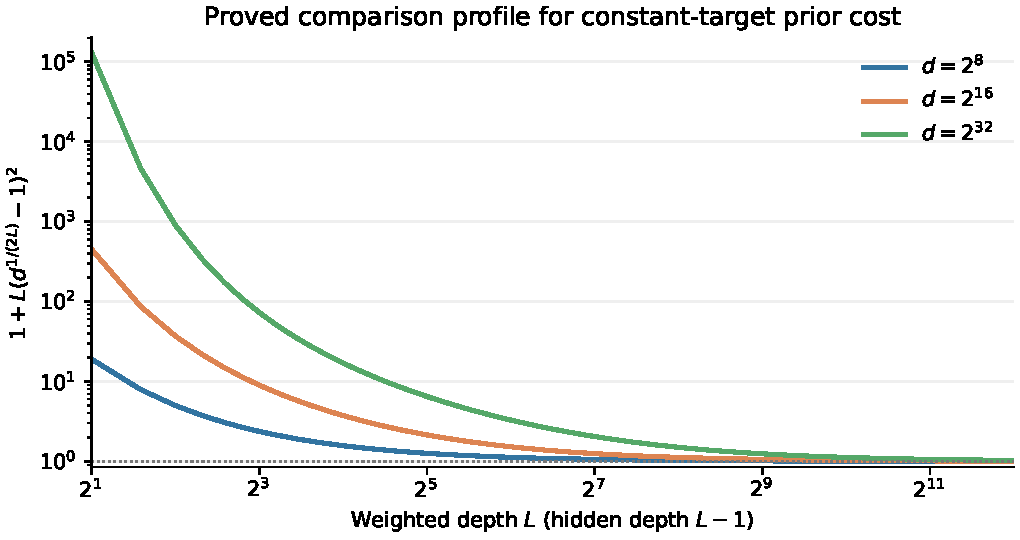
\includegraphics[width=.94\textwidth]{figures/critical-constant-depth-profile.pdf}
\caption{The comparison function in the all-depth constant-target theorem.
The actual critical rate lies between universal constant multiples of
this function; the curves are not numerical estimates of that rate.
The shallow-depth growth and the transition to bounded cost are parts
of one quantitative statement. Depth counts weighted layers.}
\label{fig:critical-constant-profile}
\end{figure}

\section{A strict target-relative ordering at depth two}
\label{sec:critical-shallow-ordering}

The common limiting rate does not imply equality at finite depth.
At depth two one can determine a strict comparison between simple
targets and every nontrivial parity.

\begin{theorem}[Constants have lower critical rate than nontrivial parities]
\label{thm:critical-shallow-parity-ordering}
At critical scaling and depth $L=2$, let $\mathbf1$ denote the
constant-positive Boolean function. If $f$ is nonconstant and
antipodally even, meaning $f(-x)=f(x)$, then
\[
 J_2(f)>J_2(\mathbf1).
\]
Consequently every parity of degree at least two has strictly larger
critical rate than a constant or a dictator. The negative constant
and signed dictators have the same rate as $\mathbf1$.
\end{theorem}

Write
\[
 X_f(W)=\frac1m\sum_{x\in\{-1,1\}^d}
                 f(x)\tanh(W\cdot\bar x),\qquad m=2^d.
\]
The proof uses the following exact formula for character targets.

\begin{lemma}[Depth-two character rate]
\label{lem:critical-character-cramer}
If $f$ is a Boolean character, including the constant character, then
\[
 J_2(f)=\max_{t\ge0}\left\{
 \frac t2-\log\mathbb E_W
                 \exp\left(\frac{t^2X_f(W)^2}{2}\right)\right\}.
\]
The maximizing parameter for the constant character exists and is
strictly positive. For an arbitrary Boolean $f$, the right-hand side
is a lower bound for $J_2(f)$.
\end{lemma}

\begin{proof}
At depth two, the output vector has the distribution
\[
 z_N=\frac1N\sum_{i=1}^N Z_i h(W_i),\qquad
 h(W)(x)=\tanh(W\cdot\bar x),
\]
where $Z_i\sim\mathcal N(0,1)$ are independent of the first-layer
weights. Its logarithmic moment generating function is
\[
 \Lambda(\theta)=
 \log\mathbb E_W\exp\{(\theta\cdot h(W))^2/2\}.
\]
It is finite for every $\theta$. The depth-two output rate is the
convex Legendre transform
$I(z)=\sup_\theta(\theta\cdot z-\Lambda(\theta))$.
This also follows directly from the variational functional: among
joint laws of $(h,Z)$ having a given marginal $\nu$ and
$\mathbb E[Zh]=z$, the minimum relative entropy in the Gaussian
$Z$ coordinate is $z^TQ(\nu)^+z/2$. Minimizing the remaining
marginal entropy gives precisely the entropy formula for $I$.

For completeness the rate is finite and continuous on the whole
output space. The first feature covariance $K$ is positive definite.
Jensen's inequality gives
$\Lambda(\theta)\ge\mathbb E(\theta\cdot h)^2/2
\ge\lambda_{\min}(K)\|\theta\|_2^2/2$. Thus its dual is finite;
the Gaussian scalar also makes every output direction available.
Equivalently, the finite-dimensional entropy duality here has no
boundary obstruction. Strict or non-strict output margins consequently
give the same infimum.

The law of the output vector is invariant under input translations
$x\mapsto sx$ and under global output negation. For a character $f$,
the transformation $z(x)\mapsto f(s)z(sx)$ preserves both this law
and the constraints $f(x)z(x)\ge1/2$. Averaging over all $s$ and
using convexity replaces any feasible $z$ by $af$, where
$a=m^{-1}\sum_xf(x)z(x)\ge1/2$, without increasing $I$.
Convexity and $I(0)=0$ then reduce the optimum to $z=f/2$.
The same group averaging in the dual restricts $\theta$ to
$tf/m$, giving the displayed formula. Symmetry in $t$ permits
$t\ge0$. For general $f$, substituting this dual vector directly
gives the asserted lower bound, because
$\theta\cdot z\ge t/2$ on the target-margin event.

For the constant character, $X_{\mathbf1}$ is nonzero with positive
probability. Therefore for some $a,p>0$,
$\Pr\{|X_{\mathbf1}|\ge a\}\ge p$, and the objective tends to
$-\infty$ as $t\to\infty$. Its derivative at zero is $1/2$.
It has a finite, strictly positive maximizer.
\end{proof}

\begin{proof}[Proof of Theorem~\ref{thm:critical-shallow-parity-ordering}]
Write $W\cdot\bar x=b+w\cdot x$. For every real $u$,
\[
 \tanh(b+u)+\tanh(b-u)
 =\frac{\sinh(2b)}{\cosh(b+u)\cosh(b-u)}.
\]
For $b\ne0$ every such antipodal pair sum is nonzero and has the
same sign as $b$. If $f$ is even and nonconstant, it takes both signs
on the set of antipodal pairs. Strict triangle inequality therefore
gives, pointwise for every finite $w$ and $b\ne0$,
\[
 |X_f(b,w)|<|X_{\mathbf1}(b,w)|.
\]
The Gaussian bias is nonzero almost surely, so for every $t>0$,
\[
 \mathbb E e^{t^2X_f^2/2}
 <\mathbb E e^{t^2X_{\mathbf1}^2/2}.
\]
Evaluate the lower bound in the preceding lemma at a positive
maximizer for the constant character. This proves the strict rate
inequality.

Every positive even-degree parity is antipodally even and nonconstant.
A parity of odd degree at least three has the same rate as a parity
of the preceding even degree by the projective coordinate symmetry.
That symmetry also identifies constants and dictators, and global
output negation identifies their negatives.
\end{proof}

The strict gap implies an exponentially small zero-data prior ratio
between such a target and a constant as width tends to infinity at
this fixed depth. It does not give a sample lower bound: a few
oppositely labeled observations already eliminate the constant
competitor. The exact ordering at every finite dimension and arbitrary
depth remains open; the preceding comparison covers growing-relevance
targets at fixed depth and sufficiently large dimension. Neither result
completely orders training-consistent extensions. The later sample lower
bound uses a separate comparison with an explicit interpolating function.

The pointwise comparison used in the proof is specific to a first-layer
feature. For example, on two input bits put
\[
 h_1=\tanh(x_1+x_2-1),\quad
 h_2=\tanh(x_1+x_2+1),\quad h_3=\tanh(1),
 \qquad g=\tanh(h_1-h_2+h_3).
\]
This uses only first-layer biases. The feature $g$ is positive when
$x_1x_2=1$ and negative when $x_1x_2=-1$: its two values are
$\tanh(2\tanh1-\tanh3)>0$ and $-\tanh(\tanh1)<0$.
Consequently its parity coefficient has greater magnitude than its
constant coefficient. Thus the preceding pointwise domination fails
already for a second-hidden-layer feature. This example does not
reverse the full prior rate comparison; it identifies a limitation of
this proof method.

\section{A polynomial sample lower bound at each fixed critical depth}
\label{sec:critical-polynomial-sample-lower}

A low-rate interpolating halfspace gives a sample lower bound for the
actual critical posterior. The bound is polynomial in the parity and
ambient dimensions, and the width limit is taken before those dimensions
grow.

\begin{lemma}[Amplifying a first-feature mean through its second moment]
\label{lem:critical-mixture-mean-seed}
Let $\mu_1$ be the uncontrolled first-feature law. Suppose a feature law
$\nu$ satisfies $D(\nu\Vert\mu_1)\le D$, where $D\ge1$, and its mean
$h$ satisfies $g(x)h(x)\ge a$ at every input, with $0<a\le1$ and
$g$ Boolean. Set $R=D/a^2$ and $q=R^{1/L}$. If $q\le D$, then
\[
 J_L(g)\le5000L R^{1/L}.
\]
\end{lemma}

\begin{proof}
Put $\theta=q/D\le1$. The first controlled law
$(1-\theta)\mu_1+\theta\nu$ has entropy at most $\theta D=q$ by
convexity, and its second moment dominates
$\theta hh^T$. Thus it has a tracked rank-one vector
$b_1=\sqrt\theta h$ with
\[
 g(x)b_1(x)\ge\sqrt\theta a=q^{-(L-1)/2}.
\]
This is a second-moment component; it need not equal the first
controlled law's mean.

For $L=2$, choose the readout $z=h/(2a)$. Its cost is at most
$1/(8\theta a^2)=q/8$, proving the assertion in this case.
Suppose $L\ge3$ and put $c=1/100$. For every $0\le v\le1$ and
$u\ge0$, the elementary estimate used in the constant-target
construction gives
\[
 \mathbb E\tanh(u+\sqrt v Z)\ge c\min\{u,1\}.
\]
At the second hidden layer shift the reference Gaussian by
$\sqrt q\,b_1$. Its mean-shift entropy is at most $q/2$, because
$Q_1\succeq b_1b_1^T$. After tanh, its actual mean $b_2$ satisfies
$g(x)b_2(x)\ge c q^{-(L-2)/2}$. Its second moment dominates
$b_2b_2^T$.

At each hidden layer $s=3,\ldots,L-1$, shift the reference Gaussian
by $(\sqrt q/c)b_{s-1}$. The entropy is at most $q/(2c^2)$, and
the new feature mean satisfies
\[
 g(x)b_s(x)\ge c q^{-(L-s)/2}.
\]
The induction uses only that every reference diagonal is at most one,
not that the diagonals or feature magnitudes are equal. If some shift
coordinate exceeds one in magnitude, the displayed minimum estimate
still gives the required lower bound. All shift vectors lie in the
corresponding covariance range; the formulas therefore also apply to
singular covariances. Tanh pushforward cannot increase the entropy.

Finally take $z=b_{L-1}/(2c q^{-1/2})$. It has the required global
margin and Gaussian readout cost at most $q/(8c^2)$. Summing all
costs gives the claimed bound.
\end{proof}

\begin{lemma}[A low-rate majority interpolant for parity samples]
\label{lem:critical-oriented-majority}
Let the labels be a parity on a nonempty coordinate set $S$, and draw
$n\ge1$ independent uniform cube inputs. Fix one $i_0\in S$ and an
odd number $m\le d-1$ of other coordinate indices $I$.
There is a sample-dependent Boolean majority function
\[
 g(x)=\operatorname{sign}\!\left(\sum_{j\in I}s_jx_j\right),
 \qquad s_j\in\{-1,1\},
\]
which fits every training label with probability at least
$1-n\exp[-m/(6n)]$.
For every sample, this function admits a first-feature law $\nu$ with
\[
 D(\nu\Vert\mu_1)\le dm,
 \qquad g(x)\mathbb E_\nu H(x)\ge1/100
       \quad\text{for every input }x.
\]
Consequently, whenever $dm\ge10000$,
\[
 J_L(g)\le5000L(10000dm)^{1/L}
       \qquad(L\ge2).
\]
\end{lemma}

\begin{proof}
Write $Y_i$ for the parity label of training row $i$, and choose
\[
 s_j=\operatorname{sign}\!\left(\sum_{i=1}^nY_iX_{ij}\right),
\]
with either fixed convention for a zero sum.
Conditional on the entire label vector $Y$, all coordinate columns
other than $i_0$ are independent uniform sign vectors: the missing
parity coordinate is uniquely determined by these columns and $Y$.
Thus $A_{ij}=Y_iX_{ij}$, for $j\in I$, are independent uniform sign
columns conditionally on $Y$.

If $T=\sum_{i=1}^n\varepsilon_i$ is a sum of independent uniform
signs, exchangeability gives
\[
 \mathbb E\left[\varepsilon_i\operatorname{sign}(T)\right]
       =\frac{\mathbb E|T|}{n}\ge\frac1{\sqrt{3n}}.
\]
Indeed $\mathbb ET^2=n$ and $\mathbb ET^4\le3n^2$, while Holder's
inequality gives
$\mathbb ET^2\le(\mathbb E|T|)^{2/3}(\mathbb ET^4)^{1/3}$.
For each training row, the variables $s_jA_{ij}$ are therefore
independent across $j$, bounded by one in absolute value, and have
mean at least $1/\sqrt{3n}$. Hoeffding's inequality bounds the
probability that their sum is nonpositive by $e^{-m/(6n)}$.
A union bound proves the training-fit probability. Dependence between
different training rows is irrelevant to that union bound.

Since $m$ is odd, the affine form defining $g$ is a nonzero integer
at every cube input, so its global signed margin is at least one.
Shift the first-row Gaussian weight mean to have coefficient $s_j$
on $I$ and zero elsewhere, including its bias. This costs exactly
$dm/2$ in relative entropy. At each input its residual Gaussian
variance is $(d+1)/d\le2$, and its feature mean is
\[
 \mathbb E\tanh\!\left(\sum_{j\in I}s_jx_j+
                       \sqrt{(d+1)/d}\,Z\right).
\]
The elementary mean-response bound from the constant-target
construction gives signed mean at least $1/100$ everywhere.
Data processing therefore proves the first-feature-law assertion.
Apply Lemma~\ref{lem:critical-mixture-mean-seed} with
$D=dm$ and $a=1/100$. Its hypothesis
$(10000D)^{1/L}\le D$ holds whenever $D\ge10000$ and $L\ge2$.
\end{proof}


\begin{theorem}[Critical parity sample lower bound]
\label{thm:critical-polynomial-sample-lower}
Fix $L\ge2$ and $0<\eta<1$. Let the target be parity on $k\le d$
specified input coordinates, and put
\[
 M=\min\{k,d^{1/(L-1)}\}.
\]
Suppose $M\to\infty$ and $1\le n\le M^{1-\eta}$. Draw $n$ independent
uniform cube inputs labeled by this parity. For all sufficiently large
$M$, with training-sample probability at least $1-1/(2M)$, the globally
margin-conditioned posterior at
$\gamma=1$ has Gibbs error tending to $1/2$ as $N\to\infty$ at
this fixed $d,L,n$. If $p_N(x)$ is its posterior probability of the
correct label, then on the same event
\[
 \liminf_{N\to\infty}\Pr_x\{p_N(x)<2/3\}\ge1/4.
\]
For full parity, this gives $n\le d^{(1-\eta)/(L-1)}$. If
$d\ge k^{L-1}$, it gives $n\le k^{1-\eta}$.
\end{theorem}

\begin{proof}
Let $m$ be the smallest odd integer at least
$12n\log(2M(n+1))$. Since $n\le M^{1-\eta}$, one has
$m=O(n\log(M+1))=o(M)\le o(d)$, so $m\le d-1$ for large $M$.
Lemma~\ref{lem:critical-oriented-majority} supplies, with probability at
least $1-1/(2M)$, a training-consistent halfspace and a first-feature
law of entropy at most $D=dm$ with mean margin $a=1/100$.

Apply Lemma~\ref{lem:critical-mixture-mean-seed}. Its hypothesis
$(D/a^2)^{1/L}\le D$ is equivalent to $D^{L-1}\ge10000$ and holds
for large $M$. The resulting training-consistent competitor has rate
at most
\[
 5000L(10000dm)^{1/L}.
\]

Any Boolean function depending on every one of the $k$ parity coordinates
has at least $k$ relevant augmented coordinates. By
Theorem~\ref{thm:critical-fixed-depth-ordering}, its critical rate is at least
\[
 \frac1{64}\min\{d^{1/(L-1)},(dk)^{1/L}\}
       =\frac1{64}(dM)^{1/L}.
\]
The ratio of the
preceding competitor upper bound to this lower bound is at most
\[
 C L\,M^{-\eta/L}[\log(M+1)]^{1/L},
\]
which tends to zero. Thus there is a positive rate gap between a
training-consistent competitor and every function retaining all
parity coordinates.

The exact finite-domain posterior-rate principle now implies that
posterior mass on the latter functions tends to zero in the width
limit. A function omitting any one parity coordinate has uniform
parity error exactly $1/2$, even if it depends on irrelevant coordinates.
This proves the Gibbs limit. Finally
$\mathbb E_xp_N(x)\to1/2$ and Markov's inequality give
$\Pr_x\{p_N(x)<2/3\}\ge1-(3/2)\mathbb E_xp_N(x)$.
\end{proof}

The theorem concerns the actual posterior, but takes width to infinity
at fixed dimension, depth, and sample size. It gives no finite-width
threshold uniform in growing dimension and no corresponding lower
bound for posterior-majority prediction at confidence threshold $1/2$.

\begin{corollary}[Slowly growing learner depth]
\label{cor:critical-growing-depth-sample-lower}
Fix $0<\eta<1$. For full parity, the same conclusion holds at sample sizes
$n\le d^{(1-\eta)/(L-1)}$ along integer depths $L=L(d)\ge2$ satisfying
\[
 L=o\!\left(\sqrt{\frac{\log d}{\log\log d}}\right).
\]
For each $d$, the width limit is taken with its corresponding $L(d)$
and sample size fixed.
\end{corollary}

\begin{proof}
Here $M=d^{1/(L-1)}\to\infty$. The halfspace construction has
$m\le Cn\log(M+1)=o(M)\le o(d)$ uniformly in $L\ge2$ at the
specified sample sizes. Its first-feature entropy bound and amplification
are also uniform. The rate ratio is therefore at most
\[
 C L\,d^{-\eta/[L(L-1)]}[\log(d+1)]^{1/L}
\]
with universal $C$. Its logarithm tends to minus infinity under the
stated depth assumption. The mixture hypothesis and the training
success probability also hold uniformly, so the same rate-gap argument
applies.
\end{proof}

\section{Parity remains hard at nearly logarithmic learner depth}
\label{sec:critical-nearly-logarithmic-depth}

The comparison can be extended to a larger growing-depth range by
retaining the leading constant in both the interpolating competitor's
rate and the transport lower bound. The first improvement comes from
tracking the freely cooling feature variance during mean amplification.
It avoids charging a fixed loss at every hidden layer.

\begin{lemma}[Mean amplification with its leading constant]
\label{lem:critical-sharp-mean-amplification}
Fix $a\in(0,1]$. Suppose a first-feature law $\nu$ has entropy at most
$D\ge1$ relative to the unmodified first-feature law $\mu$, and its
mean $h$ satisfies $g(x)h(x)\ge a$ everywhere, for a Boolean $g$.
Put $q=(D/a^2)^{1/L}$. There are constants $K,P,C$, depending only on
$a$, such that, if $L\ge2$ and $q\ge KL^P$, then
\[
 J_L(g)\le\frac q2\{L+C\log L\}.
\]
The first law and the subsequent covariance diagonals need not be
constant over inputs.
\end{lemma}

\begin{proof}
Let $F(v)=\mathbb E\tanh^2(\sqrt vZ)$ and $u_s=F^s(2)$.
The function $F$ is nondecreasing and one-Lipschitz. Monotonicity is
pointwise in $v$, and Gaussian differentiation gives $F'\le1$ because
$(\tanh^2)''\le2$. On $[0,2]$, one has $v-F(v)\ge cv^2$ with
universal $c>0$: the ratio tends to two at zero and is strictly
positive away from zero. It follows that
\[
 u_1<1,\qquad u_s\le\frac{C_0}{s+1},\qquad
 \sum_{s=1}^L u_s\le C_1\log(L+1).
\]
For a centered Gaussian $G$ of variance $v$, the same second-derivative
bound and symmetry give
\[
 \mathbb E\tanh^2(G+t)\le F(v)+t^2.
\]
For $t\ge0$, integration of
$\mathbb E\operatorname{sech}^2(G+s)\ge1-v-s^2$ gives the convenient
weaker estimate
\[
 \mathbb E\tanh(G+t)\ge t(1-v-t^2).
\]

Set $\theta=q/(2D)=1/(2a^2q^{L-1})$.
Use $(1-\theta)\mu+\theta\nu$ at the first hidden layer. Its entropy
is at most $q/2$, and its second moment dominates $b_1b_1^T$ with
$b_1=\sqrt\theta h$. Its maximum diagonal is at most $u_1+\theta$.
For $L=2$, a readout proportional to $b_1$ costs at most $q/4$,
proving the assertion. Assume henceforth $L\ge3$.

Let $\kappa=1-u_1>0$, $\epsilon=\kappa/(8L^2)$, and
\[
 c_s=1-u_{s-1}-\epsilon\qquad(2\le s\le L-1).
\]
These constants are uniformly positive. The preceding bounds on $u_s$
imply, for universal constants $A_0,C_2$,
\[
 \prod_{s=2}^{L-1}c_s^{-1}\le L^{A_0},\qquad
 \sum_{s=2}^{L-1}c_s^{-2}\le L-2+C_2\log L.
\]
Indeed, $-\log c_s$ and $c_s^{-2}-1$ are both at most a universal
multiple of $u_{s-1}+\epsilon$.

At hidden layer $s$, shift the reference Gaussian by
\[
 m_s(x)=\frac{\sqrt q}{c_s}b_{s-1}(x),
\]
and let $b_s$ be its tanh feature mean. For $s=2$, $b_1$ denotes
the tracked component just constructed; thereafter $b_{s-1}$ is the
actual preceding mean. In either case its outer product is dominated
by the preceding second moment. Thus the shift lies in the covariance
range and costs at most $q/(2c_s^2)$, including singular references.

The centered-Gaussian mean $\mathbb E\tanh(G+t)$ is odd, has the sign
of $t$, and has absolute value at most $|t|$. Therefore, without yet
using a variance bound,
\[
 \max_x|m_s(x)|
 \le\frac{L^{A_0}}{\sqrt2a}\,q^{-(L-s)/2}.
\]
For $q\ge2$, summing the resulting geometric series gives
\[
 \theta+\sum_{s=2}^{L-1}\max_x|m_s(x)|^2
 \le C_a L^{2A_0}/q.
\]
Choose $K,P$ so that $q\ge KL^P$ makes this at most $\epsilon$;
the same choice ensures $\theta\le1$.
Since $F$ is one-Lipschitz, the shifted-square estimate gives inductively
\[
 \max_x Q_s(x,x)
 \le u_s+\theta+\sum_{t=2}^s\max_x|m_t(x)|^2.
\]
In particular the variance error before layer $s$, together with the
squared current shift, is at most $\epsilon$.
The shifted-mean estimate consequently yields
\[
 g(x)b_s(x)\ge c_s g(x)m_s(x)
             =\sqrt q\,g(x)b_{s-1}(x).
\]
The last hidden mean has global signed margin at least
\[
 \sqrt\theta a q^{(L-2)/2}=\frac1{\sqrt{2q}}.
\]
A readout proportional to this mean has output margin $1/2$ and costs
at most $q/4$. Adding all costs gives
\[
 \frac q2+\frac q2\sum_{s=2}^{L-1}c_s^{-2}+\frac q4
 \le\frac q2\{L+C\log L\},
\]
as required.
\end{proof}

\begin{lemma}[Joint optimization of the transport budget]
\label{lem:critical-joint-budget}
If a Boolean function depends on all $d$ original input coordinates,
then any admissible critical path of cost $A$ satisfies, for every $t>0$,
\[
 d\le8(2+1/t)^{L-2}
 \left(\frac{A+(L-2)t}{L-1}\right)^{L-1}
 \exp\!\left(2\sqrt{2A/d}\right).
\]
In particular, if $A\le(q/2)\{L+C\log L\}$, then
\[
 d\le4q^{L-1}
 \exp\!\left(C'\log L+C'L/\sqrt q+2\sqrt{2A/d}\right),
\]
where $C'$ depends only on $C$.
\end{lemma}

\begin{proof}
Use the sharper pathwise transport inequality
\eqref{eq:critical-transport-exact-budget}, with readout cost $r$,
hidden costs $D_s$, and $k\ge d$ relevant augmented coordinates.
Cauchy--Schwarz gives
\[
 (1+\sqrt{2D_s})^2\le(2+1/t)(D_s+t).
\]
The arithmetic-geometric mean inequality gives
\[
 r\prod_{s=2}^{L-1}(D_s+t)
 \le\left(\frac{A+(L-2)t}{L-1}\right)^{L-1}.
\]
The first-layer factor is at most $\exp(2\sqrt{2A/d})$.
Combining these facts proves the first display, also when $L=2$ and
the products are empty. For the second choose $t=\sqrt q$, factor out
$2^{L-2}$ and $(q/2)^{L-1}$, and use
$\log(1+u)\le u$. The resulting errors are bounded by
$C'\log L+C'L/\sqrt q$.
\end{proof}

\begin{theorem}[Critical parity lower bound at nearly logarithmic depth]
\label{thm:critical-nearly-logarithmic-depth}
Fix $0<\eta<1$. Let the target be full parity on $d$ coordinates and
let integer depths $L=L(d)\ge2$ satisfy
\[
 L=o\!\left(\frac{\log d}{\log\log d}\right).
\]
Put $M=d^{1/(L-1)}$, and draw
$1\le n\le M^{1-\eta}$ independent uniform cube inputs, labeled by
parity. For all sufficiently large $d$, with training probability at
least $1-1/(2M)$, the original globally margin-conditioned posterior at
$\gamma=1$ satisfies
\[
 \lim_{N\to\infty}\text{Gibbs error}=\frac12,
 \qquad
 \liminf_{N\to\infty}\Pr_x\{p_N(x)<2/3\}\ge\frac14.
\]
For each $d$, the width limit fixes $d,L,n$ first. Moreover, there is a
universal $c>0$ for which the same conclusion holds for every
\[
 2\le L\le c\eta\frac{\log d}{\log\log d},
\]
once $d$ is sufficiently large depending on $\eta$.
\end{theorem}

\begin{proof}
Let $m$ be the smallest odd integer at least
$12n\log(2M(n+1))$. For large $d$,
\[
 m\le50n\log M\le50M^{1-\eta}\log M=o(M)\le o(d).
\]
Lemma~\ref{lem:critical-oriented-majority} supplies, with the stated
training probability, a consistent Boolean function and a first-feature
law of entropy $D=dm$ and global signed mean at least $a=1/100$.
Put $q=(10000dm)^{1/L}$. The depth hypothesis implies
\[
 \log q\ge\frac{\log d}{L}\gg\log\log d,
\]
so $q$ exceeds every fixed power of $L$.
Lemma~\ref{lem:critical-sharp-mean-amplification} gives a consistent
competitor of rate at most $U=(q/2)\{L+C\log L\}$.

Suppose a Boolean function retaining all $d$ coordinates had rate at
most $U$. Apply Lemma~\ref{lem:critical-joint-budget} to paths whose
costs approach its infimum, then use continuity and monotonicity in
the budget. It follows that
\[
 \log\frac d{q^{L-1}}
 \le\log4+C'\log L+C'L/\sqrt q+2\sqrt{2U/d}.
\]
The last two terms tend to zero. For $L\ge3$, use $m\le d$,
$q\le(10000d^2)^{1/L}$, and $L=O(\log d)$ to see $U/d\to0$.
For $L=2$, use $m\le50d^{1-\eta}\log d$ instead.
On the other hand, the sample bound and $q^L=10000dm$ give
\[
 \log\frac d{q^{L-1}}
 \ge\frac{\eta\log d}{L}-\log(500000\log M).
\]
Here the first term dominates $\log\log d$, whereas the other
logarithmic terms are $O(\log\log d)$. This is a contradiction.
There is therefore a strict rate gap between the consistent competitor
and every Boolean function retaining all $d$ input coordinates.

The exact finite-domain posterior rate principle makes posterior mass
on the latter class tend to zero. Every remaining function omits a
parity coordinate and has uniform parity error exactly $1/2$.
This proves the Gibbs limit, and Markov's inequality gives the displayed
confidence-error bound from $\mathbb E_xp_N(x)\to1/2$.

For the final depth range, choose the universal $c$ small enough that
$\log q\ge\log d/L$ guarantees the fixed power of $L$ required by
the amplification lemma, and that
$\eta\log d/L$ exceeds $(C'+2)\log\log d$ by a fixed factor.
This is possible independently of $\eta\le1$.
The remaining estimates hold for all sufficiently large $d$ depending
on $\eta$, completing the proof.
\end{proof}

This theorem concerns the actual posterior, including mixtures of
minimizers. It does not reach the order-$\log^2d$ depths at which
controlled parity seeds attain a bounded absolute rate, and it does
not by itself give an exponential-in-teacher-depth lower bound.

\section{The exact first-order scalar entrance cost}
\label{sec:critical-scalar-expansion}

\begin{theorem}[Small-variance scalar expansion]
\label{thm:critical-scalar-expansion}
There are universal constants $q_0,C>0$ such that
\[
 \bigl|V(q)-(V_*-2q)\bigr|\le Cq^2
 \qquad(0<q\le q_0).
\]
In particular, $\lim_{q\downarrow0}(V_*-V(q))/q=2$.
\end{theorem}

\begin{proof}
We first construct a nearly optimal small-state bridge. At state
$q$, replace the reference Gaussian by
$\mathcal N(0,(1+4q)q)$. Since
\[
 F(u)=u-2u^2+O(u^3),
\]
its new state $q'$ and entropy cost $D$ satisfy
\[
 q'=q+2q^2+O(q^3),\qquad
 D=\tfrac12[4q-\log(1+4q)]=4q^2+O(q^3).
\]
For sufficiently small $q$, therefore,
\[
 q'-q\ge q^2,\qquad
 D\le(2+Cq)(q'-q).
\]
Starting at any $0<a<b$ in this small interval, take full steps
while they remain below $b$. The states reach the final interval
in finitely many steps, since every increment is at least $a^2$.
The full-step costs sum to at most
$2(b-a)+Cb^2$. On the last step reduce the variance inflation
continuously to hit $b$ exactly; its entropy is at most $Cb^2$.
Thus, after changing $C$, there is a bridge from $a$ to $b$ of cost
\begin{equation}\label{eq:critical-sharp-scalar-bridge}
 2(b-a)+Cb^2.
\end{equation}
Appending a nearly optimal path from $q$ and letting $a\downarrow0$
proves
\[
 V_*-V(q)\le2q+Cq^2.
\]

For the reverse inequality take $q$ still smaller, and start a
near-optimal scalar path at $0<a<q$. Its cost may be assumed less
than two, by the uniform upper bound for $V$. It must cross level
$q$: otherwise the readout alone costs more than $1/(8q)>2$.
Let $b$ be its first state at or above $q$, and $a_-$ the preceding
state. Then $a_-<q$. The crossing satisfies $b<8q$. Indeed the
preactivation second moment is at least $b$, because
$\tanh^2z\le z^2$. At a ratio $r=b/a_-\ge8$, Gaussian entropy
duality gives a single-step cost at least
\[
 \tfrac12(r-1-\log r)
 \ge\tfrac12(8-1-\log8)>2,
\]
contrary to the total-cost bound.

The scalar exponential potential with coefficient two gives prefix
entropy at least $2(b-a)$. The remaining path costs at least $V(b)$.
Apply the bridge~\eqref{eq:critical-sharp-scalar-bridge} from $q$
to $b$, which stays in the small-state interval since $b<8q$:
\[
 V(b)\ge V(q)-2(b-q)-Cb^2.
\]
The entire path therefore costs at least
\[
 V(q)+2q-2a-64Cq^2.
\]
Taking the infimum over near-optimal paths and then $a\downarrow0$
gives $V_*-V(q)\ge2q-C''q^2$, proving the theorem.
\end{proof}

The coefficient two describes the scalar entrance to the common
rare-event trajectory. It does not identify the function-dependent
cost of bringing a particular target direction to that scalar regime.
Thus it is an ingredient for a possible target-relative expansion,
not a characterization of the posterior's learning behavior.


\appendix
\section{An exact variational principle at the critical exponent}
\label{sec:critical-variational}

For completeness we reproduce the finite-domain variational foundation.
Here $\phi=\tanh$. For arbitrary fixed depth, the critical prior admits a direct finite-domain
large-deviation description. This result requires neither a propagation-of-chaos
assumption nor differentiability of the activation. It identifies the functional used in the critical-rate capacity constructions
with the actual Gaussian probability rate.
Covariance-process large deviations for Gaussian networks have been studied
in a more general functional setting by Andreis, Bassetti, and
Hirsch~\cite{andreis2026}. No novelty claim is made for the general
large-deviation framework; the finite-domain proof below fixes the precise
normalizations and strict-margin convention used here.

Fix $\gamma=1$, enumerate $\mathcal X=\{x^1,\ldots,x^m\}$, where $m=2^d$,
and put $r=L-1$. All limits in this section hold with $d$ and $L$ fixed.
Write $E=[-1,1]^m$ and let $\mathcal P(E)$ carry its weak topology.
For $\nu\in\mathcal P(E)$ define
\[
 K(\nu)=\int_E hh^{\mathsf T}\,d\nu(h),\qquad
 Q_0(a,b)=\frac{\bar x^a\cdot\bar x^b}{d}.
\]
For any positive semidefinite $m\times m$ matrix $Q$, let
\[
 \mathsf T_Q(u)=\bigl(\phi((Q^{1/2}u)_a)\bigr)_{a=1}^m,
 \qquad
 \mathsf M_Q=(\mathsf T_Q)_\#\mathcal N(0,I_m).
\]
Here $T_\#\rho$ is the distribution of $T(U)$ when $U$ has distribution $\rho$,
and $Q^{1/2}$ is the positive semidefinite square root. Relative entropy is
\[
 D(\nu\Vert\rho)=
 \begin{cases}
 \displaystyle\int\log\frac{d\nu}{d\rho}\,d\nu,&\nu\ll\rho,\\
 +\infty,&\text{otherwise}.
 \end{cases}
\]
Finally define the Gaussian energy
\[
 \mathcal G_Q(z)=
 \begin{cases}
 \frac12 z^{\mathsf T}Q^+z,&z\in\operatorname{range}(Q),\\
 +\infty,&z\notin\operatorname{range}(Q),
 \end{cases}
\]
where $Q^+$ is the Moore--Penrose inverse.

\begin{theorem}[Critical finite-domain large deviations]
\label{thm:critical-ldp}
Let $Z_N=(z_w(x^a))_{a=1}^m$ under the unconditioned prior
$\mu_{N,1}$. The sequence $Z_N$ satisfies a large-deviation principle
with speed $N$ and good rate function
\begin{equation}\label{eq:critical-rate}
 \begin{split}
 I(z)=\inf_{\nu_1,\ldots,\nu_r\in\mathcal P(E)}
 \bigg\{&D(\nu_1\Vert\mathsf M_{Q_0})
  +\sum_{s=2}^{r}D\bigl(\nu_s\Vert\mathsf M_{K(\nu_{s-1})}\bigr)
  +\mathcal G_{K(\nu_r)}(z)\bigg\}.
 \end{split}
\end{equation}
In particular, for every open $O\subseteq\mathbb R^m$ and closed
$F\subseteq\mathbb R^m$,
\[
 -\inf_{z\in O}I(z)
 \leq\liminf_{N\to\infty}\frac1N\log\Prb(Z_N\in O),
 \qquad
 \limsup_{N\to\infty}\frac1N\log\Prb(Z_N\in F)
 \leq-\inf_{z\in F}I(z).
\]
The infimum in \eqref{eq:critical-rate} is attained whenever it is finite.
No covariance matrix in the statement is required to be nonsingular.
\end{theorem}

\begin{proof}
We give an exact representation of the finite-width law and then apply
Sanov's theorem and continuous contraction~\cite{dembozeitouni}.

Let $\Gamma_m=\mathcal N(0,I_m)$. Independently for each
$s=1,\ldots,r$, let $U_{s,1},\ldots,U_{s,N}$ have law $\Gamma_m$, and set
\[
 \eta_{s,N}=\frac1N\sum_{i=1}^N\delta_{U_{s,i}}.
\]
Also let $V_N=G/\sqrt N$, where $G\sim\Gamma_m$ is independent of these
empirical measures. Recursively define
\[
 \nu_{1,N}=(\mathsf T_{Q_0})_\#\eta_{1,N},\qquad
 \nu_{s,N}=(\mathsf T_{K(\nu_{s-1,N})})_\#\eta_{s,N}\quad(2\leq s\leq r).
\]
These are exactly the joint laws of the network's empirical hidden-activation
vectors on $\mathcal X$. Indeed, first-layer preactivation vectors are
independent Gaussians with covariance $Q_0$. Conditional on the preceding
layer, each subsequent row of weights gives an independent Gaussian vector
with covariance
\[
 \frac1N\sum_{i=1}^N
 \bigl(h_i^{s-1}(x^a)h_i^{s-1}(x^b)\bigr)_{a,b}
 =K(\nu_{s-1,N}).
\]
The conditional distribution depends on the previous layer only through its
empirical measure. Finally, readout weights have variance $N^{-2}$, so
\begin{equation}\label{eq:critical-output-representation}
 Z_N\ \stackrel{\mathrm{law}}{=}\ K(\nu_{r,N})^{1/2}V_N.
\end{equation}
This representation is exact for every $N$.

Sanov's theorem on $\mathcal P(\mathbb R^m)$ gives the good rate
$D(\eta\Vert\Gamma_m)$ for each $\eta_{s,N}$. The elementary Gaussian
large-deviation principle gives rate $\|v\|_2^2/2$ for $V_N$.
Independence and the finite-product principle therefore give the good rate
\[
 \sum_{s=1}^r D(\eta_s\Vert\Gamma_m)+\frac12\|v\|_2^2
\]
for $(\eta_{1,N},\ldots,\eta_{r,N},V_N)$.

The recursive map from these variables to $(\nu_1,\ldots,\nu_r,z)$ is
continuous. To verify the only potentially delicate point, suppose
$Q_j\to Q$ and $\eta_j\Rightarrow\eta$ weakly. For every continuous
$b:E\to\mathbb R$, the functions $b\circ\mathsf T_{Q_j}$ converge
uniformly on each compact subset of $\mathbb R^m$ to
$b\circ\mathsf T_Q$, since matrix square roots are continuous and $\phi$
is continuous. Their absolute values are uniformly bounded. Tightness of a
weakly convergent sequence of probability measures then gives
\[
 \int b\circ\mathsf T_{Q_j}\,d\eta_j
 \longrightarrow\int b\circ\mathsf T_Q\,d\eta.
\]
Also $\nu\mapsto K(\nu)$ is continuous because every coordinate
$h_ah_b$ is continuous and bounded on $E$. This proves continuity of the
whole recursive map, including \eqref{eq:critical-output-representation}.

Continuous contraction now gives the rate by minimizing over its preimages.
For a measurable map $T$ and a reference probability $\rho$, the entropy
contraction identity is
\begin{equation}\label{eq:entropy-contraction-identity}
 \inf_{\eta:T_\#\eta=\nu}D(\eta\Vert\rho)
 =D(\nu\Vert T_\#\rho).
\end{equation}
The lower bound is data processing. When the right side is finite and
$q=d\nu/d(T_\#\rho)$, the measure $d\eta=q(T(u))\,d\rho(u)$ attains
equality. If the right side is infinite, data processing already proves
the identity in the extended real sense. Apply
\eqref{eq:entropy-contraction-identity} successively with
$T=\mathsf T_{Q_0}$ and $T=\mathsf T_{K(\nu_{s-1})}$.
The last minimization is
\[
 \inf_{v:Q^{1/2}v=z}\frac12\|v\|_2^2=\mathcal G_Q(z),
\]
including singular $Q$. This proves \eqref{eq:critical-rate}.

The contraction theorem supplies a good rate and exponential tightness.
For completeness, the displayed minimization is also directly well behaved:
relative entropy is jointly lower semicontinuous, the map
$\nu\mapsto\mathsf M_{K(\nu)}$ is weakly continuous, and
\[
 \mathcal G_Q(z)=\sup_{t\in\mathbb R^m}
 \left\{t^{\mathsf T}z-\frac12t^{\mathsf T}Qt\right\}
\]
is jointly lower semicontinuous in $(Q,z)$. Since $\mathcal P(E)^r$ is
compact, every finite infimum in \eqref{eq:critical-rate} is attained.
Moreover $K(\nu)\preceq mI_m$, so $I(z)\geq\|z\|_2^2/(2m)$.
\end{proof}

\begin{corollary}[Full-margin masses and posterior rates]
\label{cor:critical-margin-rates}
For a Boolean function $f$, regarded as a vector in $\{-1,1\}^m$, set
\[
 J(f)=\inf_{z:\ f_a z_a\geq1/2\ \forall a}I(z).
\]
Then the strict-margin event used throughout this paper has the exact rate
\begin{equation}\label{eq:critical-full-margin-rate}
 \lim_{N\to\infty}-\frac1N\log\mu_{N,1}(A_{N,f})=J(f).
\end{equation}
For a fixed noiseless training set $S$, let $\mathcal B_S$ be the Boolean
functions agreeing with its labels. If
$J_S=\min_{g\in\mathcal B_S}J(g)<\infty$, the actual globally conditioned
posterior satisfies, for every $f\in\mathcal B_S$,
\[
 \lim_{N\to\infty}-\frac1N\log\Pi_{N,1}(f\mid S)=J(f)-J_S.
\]
In particular, posterior mass concentrates on the minimizers of $J$ within
$\mathcal B_S$. These logarithmic asymptotics do not determine how mass is
divided between tied minimizers.
\end{corollary}

\begin{proof}
For $c\geq1$, retaining any feature laws in \eqref{eq:critical-rate} and
scaling only the output gives
\[
 I(cz)\leq c^2 I(z),
\]
because the entropy terms are nonnegative and the Gaussian energy scales
quadratically. If $f_a z_a\geq1/2$ for all $a$, then $cz$ has strict
margin for every $c>1$. Letting $c\downarrow1$ shows that the infimum of
$I$ over the open strict-margin orthant equals its infimum over the
closed orthant. The lower and upper large-deviation bounds therefore agree,
proving \eqref{eq:critical-full-margin-rate}.

Conditioning the prior on the global margin event and subsequently on the
labels gives exactly
\[
 \Pi_{N,1}(f\mid S)=
 \frac{\mu_{N,1}(A_{N,f})}
 {\sum_{g\in\mathcal B_S}\mu_{N,1}(A_{N,g})}.
\]
For fixed $d$ this is a finite sum, whose exponential rate is the smallest
$J(g)$ among its terms. This proves the ratio formula and concentration
claim.
\end{proof}



\begin{thebibliography}{9}
\bibitem{karpinski1997}
M. Karpinski and A. Macintyre.
Polynomial bounds for VC dimension of sigmoidal and general Pfaffian
neural networks.
\emph{Journal of Computer and System Sciences} 54(1), 169--176, 1997.
\url{https://doi.org/10.1006/jcss.1997.1477}.
\bibitem{hesse2002}
W. Hesse, E. Allender, and D. A. Mix Barrington.
Uniform constant-depth threshold circuits for division and iterated multiplication.
\emph{Journal of Computer and System Sciences} 65(4), 695--716, 2002.
\url{https://doi.org/10.1016/S0022-0000(02)00025-9}.
\bibitem{andreis2026}
L. Andreis, F. Bassetti, and C. Hirsch.
LDP for the covariance process in fully connected Gaussian neural networks.
\emph{Electronic Journal of Probability} 31, 2026.
\url{https://doi.org/10.1214/26-ejp1477}.
\bibitem{dembozeitouni}
A. Dembo and O. Zeitouni.
\emph{Large Deviations Techniques and Applications}. Second edition,
Springer, 1998.
\bibitem{talagrand}
M. Talagrand.
Transportation cost for Gaussian and other product measures.
\emph{Geometric and Functional Analysis} 6, 587--600, 1996.
\end{thebibliography}
\end{document}
